\documentclass[ 11pt, a4paper, twoside, openright ]{memoir}
\usepackage{xltxtra}
\usepackage{xgreek}
\setmainfont[Mapping=tex-text]{GFS Artemisia}
\usepackage{subfig}
\usepackage{algorithmic}
\usepackage{acronym}
\usepackage{listings}
\usepackage{amsfonts}
\usepackage{gr-acrnm}
\usepackage{a4wide}
\usepackage{amsmath}
\usepackage{siunitx}



%Use the hyperref package in order to create hyper-references
%If dvipdfm method is choosen, then the .dvi file must be compiled
%with the dvipdfm utility
%\usepackage[dvipdfm, bookmarks=false, linkbordercolor={1 1 1}, colorlinks=false, urlcolor={1 1 1}, urlbordercolor={1 1 1}, citecolor={1 1 1}, citebordercolor={1 1 1}, breaklinks=true pdfborder={0 0 0}]{hyperref}
\usepackage[xetex, bookmarks=false, colorlinks=true, linkcolor=black, citecolor=black, filecolor=black, urlcolor=black, breaklinks=true pdfborder={0 0 0}]{hyperref}


%Memoir package has an internal implementation of the fancyhdr package
%\usepackage{fancyhdr}

%For error suppressing
\renewcommand{\rm}{}
\renewcommand{\sl}{}

%Some definitions
\newenvironment{dedication}{\newpage\begin{flushright}\null\vskip2in}%
{\vfill\end{flushright}}

\renewcommand{\abstractnamefont}{\Huge\bfseries}

\renewcommand{\abstracttextfont}{\normalsize}

\renewcommand{\chaptermark}[1]{\markboth{\textsl{\chaptername}\ \thechapter.\ #1}{}}
\renewcommand{\sectionmark}[1]{\markright{#1}}
\newcommand{\mypagestyle}{\fancyhf{} \fancyhead{} \fancyfoot{}}

%Definitions for the wbepi (epigraphs) environment
\makeatletter
\newcommand{\wb@episource}{}
\newenvironment{wbepi}[1]{\begin{quote}\renewcommand{\wb@episource}{#1}\itshape}{\par\upshape \raggedleft %---
\textsc{\wb@episource}\\ \end{quote}}
\makeatother

\hyphenation{hete-rogeneous επε-κτεί-νουν πρό-τυ-πο προ-τει-νό-με-νες πρα-γμα-τι-κό-τη-τα ε-πε-ξερ-γα-στών κα-θυ-στέ-ρη-ση βελ-τι-στο-ποι-η-μέ-νο αρ-χι-τε-κτο-νι-κή υποτετρα-πλασιάζεται μικρο-επεξεργαστών καταχω-ρητών γραμματο-κιβωτίων χρησιμο-ποιείται προγραμμα-τιστή ελαχιστο-ποίηση προσο-μοιωτής αποτε-λέσματα αποκωδι-κοποίησης εξό-δου παραλλη-λοποίηση μοντελο-ποιούν πρα-γμα-το-ποι-εί-ται πραγματο-ποιήθηκε χρησιμο-ποιήθηκε διανυσματο-ποίησης ευθυγραμμι-σμένες διανυσμα-τικό διαπιστω-θεί διεύθυν-ση αποθηκεύο-νται υποδια-στολής προαναφερ-θείσα δρομολό-γηση συντεταγ-μένων βελτιστο-ποίηση υπολο-γισμών αρχιτε-κτονικές βελτιστο-ποιηθεί πραγμα-τικό επαναχρησι-μοποίησης βελτιστο-ποιήσεις διακλά-δωσης α-πο-θή-κευ-ση εκπό-νηση Αντωνό-πουλο επιστη-μονικές χαρακτη-ρίζεται καθι-στούν επιστημονι-κές χαρακτηρίζε-ται καθι-στούν παρα-μόρφωσης επεξεργα-στή μεταγλωττι-στών εργα-λεία επεξερ-γαστή συναρτή-σεις απαιτή-σεις απεικό-νιση δειγματο-ληψία τοποθε-τούνται συνεργα-σία αποτε-λεί υλοποί-ηση pi-xels παρατη-ρείται συνερ-γασία υλοποί-ηση κατευθύ-νονται αποκωδι-κοποίηση καταχω-ρητής φόρτω-σης επικοινω-νία Εξό-δου εκθε-τικές δεδο-μένων συστή-ματος εφαρμο-γών αντί-στοιχες διανυσμά-των δευτερό-λεπτο διανυσμα-τικούς παραλλη-λισμό ομαδοποι-ώντας παρεμβο-λής τεμαχι-σμού παρουσιά-ζεται τριγωνομε-τρικές χρησιμοποιή-θηκαν παραλλη-λισμό ομαδοποι-ώντας μεταβλη-τών παράλ-ληλη υπολογι-στικοί αποτελεσμα-τικότητα ομαδο-ποιώντας καταχώ-ρητη αντιπραγματι-σμοί ευρυγώ-νιων χρησιμοποιού-νται ξεδιπλώ-ματος πρόβλε-ψης δημιουρ-γή-θηκε εσωτε-ρικών διατίθε-ται χαρακτηρίζο-νται διατυπώνε-ται αφαίρε-σης λαμβάνο-νται πε-ρί-πτω-ση κατα-σκευή επιβάρυν-ση διαθέσι-μων διαθέσι-μους διαθέσι-μα χωρίζο-νται παραλληλι-σμού επεξεργα-στές περιγράφε-ται πραγματοποι-ούνται ετερογε-νή δημιουργού-νται τεχνολο-γίας βιβλιοθή-κης αλγορίθ-μου επεξεργα-στής παράγο-ντας προσφέ-ρει παραμόρφω-ση λανθασμέ-νης πλεονέ-κτημα φω-το-γρα-φία δια-κλα-δώ-σε-ων ε-φαρ-μο-γής δια-θέ-σι-μα ε-ντο-λών υ-πο-λο-γι-σμούς υ-πο-λο-γι-σμού πα-ρα-μόρ-φω-ση ταυ-τό-χρο-να}

\setcounter{tocdepth}{2}

\abstractintoc

%For the nomenclature
\begin{document}

\frontmatter

%Include the dedication page
%\thispagestyle{plain}
\begin{dedication}
\emph{Στην οικογένειά μου και στους φίλους μου}
\end{dedication} 

%Include the page for the acknowledgements
%\include{Acknowledgements/acknowledgements}

%\tableofcontents*
%\newpage
%\listoftables
%\newpage
%\listoffigures
%\newpage
%\chapter{Κατάλογος Συντομογραφιών}
\begin{acronym}[CESOF]
\acro{API}{Application Programming Interface}
\acro{ALF}{Accelerated Library Framework}
\acro{ASIC}{Application Specific Instruction Set}
\acro{BEI}{Broadband Engine Interface}
\acro{BIC}{Broadband Interface Controller}
\acro{BRU}{Branch Unit}
\acro{CAD}{Computer Aided Design}
\acro{CBE}{Cell Broadband Engine}
\acro{CBEA}{Cell Broadband Engine Architecture}
\acro{CESOF}{CBE Embedded SPE Object Format}
\acro{CPI}{Cycles Per Instruction}
\acro{CPU}{Central Processing Unit}
\acro{DLP}{Data Level Parallelism}
\acro{DMA}{Direct Memory Access}
\acro{DSP}{Digital Signal Processing}
\acro{EIB}{Element Interconnect Bus}
\acro{ESL}{Electronic System Level}
\acro{FoV}{Field of View}
\acro{FPGA}{Field Programmable Gate Array}
\acro{fps}{Frames per Second}
\acro{FPU}{Floating Point Unit}
\acro{FSB}{Front-Side Bus}
\acro{FXU}{Fixed-Point Unit}
\acro{GFlops}{Giga Floating-Point operations per second}
\acro{HDL}{Hardware Description Languages}
\acro{IIC}{Internal Interrupt Controller}
\acro{ILP}{Instruction Level Parallelism}
\acro{IOC}{I/O Controller}
\acro{LS}{Local Store}
\acro{LSU}{Load and Store Unit}
\acro{IU}{Instruction Unit}
\acro{MFC}{Memory Flow Controller}
\acro{MIC}{Memory Interface Controller}
\acro{MIMD}{Multiple Instruction Multiple Data}
\acro{MMU}{Memory Management Unit}
\acro{PPE}{Power Processing Element}
\acro{PPSS}{PowerPC processor Storage Subsystem}
\acro{PPU}{PowerPC Processing Unit}
\acro{PSNR}{Peak Signal to Noise Ratio}
\acro{RISC}{Reduced Instruction Set Computer}
\acro{ROI}{Region Of Interest}
\acro{sDFG}{Streaming Data Flow Graph}
\acro{SDK}{Software Development Kit}
\acro{SIMD}{Single Instruction Multiple Data}
\acro{SMP}{Symmetric Multiprocessing}
\acro{SMT}{Simultaneous Multithreading}
\acro{SoC}{System on Chip}
\acro{SPE}{Synergistic Processing Element}
\acro{SPU}{Synergistic Processing Unit}
\acro{SRAMs}{Static Random Access Memories}
\acro{SSE}{Streaming SIMD Extensions}
\acro{TLP}{Thread Level Parallelism}
\acro{VLSI}{Very Large Scale Integration}
\acro{VSU}{Vector/Scalar Unit}
\acro{VXU}{Vector/SIMD Multimedia Extension Unit}
\acro{XDR}{Rambus Extreme Data Rate}
\end{acronym} 
%Include the greek abstract for the thesis
%\thispagestyle{plain}
\begin{abstract}
Οι ευρυγώνιοι φακοί, \textsl{wide-angle} ή \textsl{fisheye lenses}, χρησιμοποιούνται σε επιστημονικές εφαρμογές ή εφαρμογές εικονικής πραγματικότητας (\textsl{virtual reality}) ώστε να επεκτείνουν το πεδίο θέασης, \ac{FoV}, των συμβατικών φωτογραφικών μηχανών. Λόγω του μεγαλύτερου πεδίου θέασης, οι εικόνες που λαμβάνονται από τέτοιου είδους φακούς εμφανίζουν κάποιου είδους παραμόρφωση. Η διόρθωση παραμόρφωσης που προκαλείται από την χρήση ευρυγώνιων φακών είναι μία εφαρμογή επεξεργασίας εικόνας (\textsl{image warping application}), η οποία χρησιμοποιείται ώστε να μετατρέψει την παραμορφωμένη εικόνα από το μοντέλο των ευρυγώνιων φακών στο μοντέλο της κεντρικής προοπτικής προβολής (\textsl{central perspective space}). Η εφαρμογή χαρακτηρίζεται από ένα μη γραμμικό, συνεχούς ροής, πρότυπο προσπέλασης της μνήμης το οποίο καθιστά το εύρος ζώνης της κύριας μνήμης έναν παράγοντα ο οποίος επηρεάζει σημαντικά την απόδοση της εφαρμογής.\newline
\indent
Ο επεξεργαστής \textsl{Cell}, \ac{CBE}, είναι ένας μη συμβατικός και ετερογενής πολύ-επεξεργαστής. Η αρχιτεκτονική του επεξεργαστή \textsl{Cell} επιτρέπει την επιτάχυνση εφαρμογών με μεγάλο βαθμό παραλληλισμού τόσο σε επίπεδο νημάτων (\textsl{thread-level parallelism}) όσο και σε επίπεδο δεδομένων (\textsl{data-level parallelism}).\newline
\indent
Η παρούσα διπλωματική εργασία παρουσιάζει την υλοποίηση, βελτιστοποίηση και αξιολόγηση ενός αλγορίθμου για την διόρθωση παραμόρφωσης εικόνας, που προκαλείται από την χρήση ευρυγώνιων φακών, στον επεξεργαστή \textsl{Cell} και σε πραγματικό χρόνο. Για την επίλυση των προβλημάτων του συστήματος μνήμης εφαρμόζουμε βελτιστοποιήσεις σε επίπεδο πηγαίου κώδικα όπως η τεχνική του \textsl{tiling} για την καλύτερη εκμετάλλευση της \textsl{on-chip} μνήμης των \acp{SPE} και για την μεγιστοποίηση της επαναχρησιμοποίησης των δεδομένων εντός του \textsl{frame}. Οι προτεινόμενες βελτιστοποιήσεις καθιστούν την διόρθωση παραμόρφωσης εικόνας στον επεξεργαστή \ac{CBE} μία διαδικασία που μπορεί να πραγματοποιηθεί σε πραγματικό χρόνο ενώ επιτυγχάνεται επιτάχυνση (\textsl{speedup}) ίση με \(7.27x\), σε σύγκριση με έναν επεξεργαστή \textsl{Intel Core2 Duo}.
\end{abstract}
\vspace{0.5in}
\begin{Large}
\textbf{Λέξεις Κλειδιά:}\\
\end{Large}
Παραμόρφωση Εικόνας, Πραγματικός Χρόνος, Παράλληλος Προγραμματισμός,\\ Υπολογισμός Stencil, Cell B.E., Ετερογενείς Επεξεργαστές Πολλαπλών Πυρήνων 
%Include the english abstract for the thesis
%\thispagestyle{plain}
\def\abstractname{Abstract}
\begin{abstract}
\end{abstract}
\vspace{0.5in}
\begin{Large}
\textbf{Keywords:}\\
\end{Large}
Vector Quantization, Entropy, Information Theory, Video Codec, Entropy Encoding, H.264, k-means 


\mainmatter
\pagestyle{Ruled}

\chapter{Εισαγωγή}
\label{chapter:chap1}

\section{Περιγραφή του Προβλήματος}
\label{section:sect11}
\indent
Οι κωδικοποιητές βίντεο είναι αναγκαίοι για να μειώσουν τον τεράστιο αριθμό δεδομένων που έχει ένα βίντεο. Σε οπτικά σήματα με ισχύ μεγαλύτερη των \si{35}{dB} δεν είναι εύκολο να παρατηρήθει διαφορά από το ανθρώπινο μάτι. Έτσι επιλέγεται να εισαχθεί ομοιόμορφος θόρυβος για να επιτευχθεί μεγαλύτερος λόγος συμπίεσης θυσιάζοντας την ποιότητα.
Η κωδικοποίηση βίντεο υλοποιείται σαν λογισμικό αλλά και στο υλικό. Οι προσωπικοί υπολογιστές συνήθιζαν να χρησιμοποιούν λογισμικό για την αναπαραγωγή βίντεο αλλά τα τελευταία χρόνια οι αύξηση των αναλύσεων του βίντεο (1080p,4K) καθιστά αδύνατη η πολύ δαπανηρή την αποκωδικοποίηση ενός συμπιεσμένου βίντεο από έναν επεξεργαστή γενικής χρήσης. Έτσι βλέπουμε υλικό ειδικά σχεδιασμένο (hardware accelerators) για κωδικοποίηση/αποκοδικοποίηση βίντεο που βοηθά τον κύριο επεξεργαστή.

\begin{figure}[h!]
    \begin{center}
        \begin{tabular}{| l | l | l | l |}
        \hline
        Χρονιά  & Κωδικοποιητής & Διάφορες Χρήσεις      & Λόγος Συμπίεσης           \\ \hline
        1993    & MPEG-1        &       VCD             &       26:1                \\ \hline
        1995    & MPEG-2        &       DVD             &       31:1                \\ \hline
        1999    & MPEG-4        &    DivX,XVid          &      200:1                \\ \hline
        2003    & H.264         & BluRay,DVB-TS         &      400:1                \\ \hline
        2013    & H.265         & next generation H.264 &      550:1                \\ \hline
        \hline
        \end{tabular}
    \end{center}

    \caption{Κυριότεροι κωδικοποιητές βίντεο!}
    \label{fig:listofcodecs}
\end{figure}

\indent
Σήμερα όπου υπάρχει βίντεο υπάρχει και κωδικοποίηση. Όπως φαίνεται στον πίνακα ~\ref{fig:listofcodecs} με το πέρασμα του χρόνου οι κωδικοποιητές γίνονταν ολοένα και πιο αποτελεσματικοί αυξάνοντας όμως κατά πολύ την πολυπλοκότητα τους. Πλέον μπορούμε με λίγα δεδομένα να έχουμε βίντεο καλής ποιότητας σε πολύ μεγάλες αναλύσεις. Ενδεικτικά για ένα ασυμπίεστο βίντεο ανάλυσης DVD (720x480) με διάρκεια 20sec και ρυθμό ανανέωσης \si{30}{Hz} χρειαζόμαστε χώρο 296ΜΒ, συμπιέζοντας το με τον H.264 θα έχουμε ένα αρχείο 0.8ΜΒ.

\section{Συμβολή της Εργασίας}
\label{section:sect12}
\indent
Στην εργασία αυτή γίνετε χρήση της κβαντοποίηση διανυσμάτων στον κωδικοποιητή H.264. Είναι μια τεχνική συμπίεσης με απώλειες οπού έχει δοκιμαστεί ελάχιστα στο βίντεο και φαίνεται πως μπορεί να δώσει λύσεις στον λόγο συμπίεσης καθώς επίσης και στην μείωση της πολυπλοκότητας του αποκωδικοποιητή. Ο τρόπος που μειώνεται η πολυπλοκότητα μπορεί να μετατρέψει ακριβά ενεργοβόρα κυκλώματα σε φθηνές μνήμες χωρίς απαιτήσεις ισχύος.

\section{Διάρθρωση της Διπλωματικής Εργασίας}
\label{section:sect13}

\indent
Στο Κεφάλαιο~\ref{chapter:chap2} παρουσιάζεται το ψηφιακό βίντεο, με ποίες μορφές αυτό αποθηκεύεται, πώς οι κωδικοποιητές το αντιμετωπίζουν και ποίες είναι οι κύριες τεχνικές που χρησιμοποιούνται για την συμπίεση του.\newline \indent

To Κεφάλαιο~\ref{chapter:chap3} αποτελεί μία σύντομη εισαγωγή στον τομέα της Θεωρίας Πληροφοριών. Είναι αναγκαίο να εξηγηθεί τι είναι η πληροφορία καθώς και η εντροπία αυτής. Επίσης θα εξηγηθεί αναλυτικά ο κύριος αλγόριθμος clustering k-means που καθώς και οι όποιες βελτιστοποίησες προέκυψαν στην πορεία.\newline \indent

Στο Κεφάλαιο~\ref{chapter:chap4} παρουσιάζονται τα βήματα που έγιναν για την παραγωγή τον κωδικών βιβλίων και την επιπλέον κατηγοριοποίηση τους με στόχο την μείωση της εντροπίας.\newline \indent

Στο Κεφάλαιο~\ref{chapter:chap5} παρουσιάζεται η επέμβαση που έγινε στον H.264 έτσι ώστε να χρησιμοποιεί τα κωδικά βιβλία για να κάνει την κωδικοποίηση/αποκωδικοποίηση.\newline \indent

Στο Κεφάλαιο~\ref{chapter:chap6} παρουσιάζονται τα αποτελέσματα του VQ-H.264 και συγκρίνονται με τις επιδόσεις του JM-H.264.

%\chapter{Ψηφιακό βίντεο και τεχνικές συμπίεσης}
\label{chapter:chap2}


\section{Εισαγωγή}
\label{section:sect21}
\indent Σε αυτό το κεφάλαιο γίνεται μία εισαγωγή στους τρόπους που οι κωδικοποιητές βίντεο διαχειρίζονται τα δεδομένα και τους τρόπους που χρησιμοποιούν για να τα συμπιέσουν. Ακόμη, σε αυτό το κεφάλαιο θα αποσαφηνιστεί γιατί το βήμα της κβαντοποίησης (εισαγωγή θορύβου) είναι αναγκαίο για να έχουμε τόσο μεγάλους λόγους συμπίεσης.

\section{Συστατικά στοιχεία του βίντεο}
\label{section:sect22}

\indent Το ψηφιακό βίντεο αποτελείται από μία σειρά καρέ που αναπαράγονται με σταθερό ρυθμό (συνήθως 25Hz η 30Hz). Το κάθε καρέ απεικονίζεται σε ένα χώρο χρωμάτων που ονομάζεται YUV, οπού το Y είναι η φωτεινότητα και το U,V η χρωματικότητα. Η κάθε συνιστώσα στο ανθρώπινο μάτι φαίνεται όπως στο Σχήμα~\ref{fig:yuv}.

\indent Σε κάθε σημείο του βίντεο (pixel) αντιστοιχίζεται μια τέτοια τιμή YUV. Υπάρχουν διάφορες μέθοδοι που γίνεται αυτή η αντιστοίχηση με κυριότερες αυτές του YUV420 και YUV444. Η πρώτη υποδεικνύει πως κάθε για κάθε τέσσερα pixel υπάρχουν τέσσερις τιμές Y, μία τιμή U και μια τιμή V. Η δεύτερη δείχνει πως για κάθε τέσσερα pixel υπάρχουν τέσσερις τιμές για την κάθε συνιστώσα π.χ για ένα καρέ ανάλυσης 720*480 τύπου YUV420 έχουμε \(720*480=345600\) στοιχεία Υ, \(720*480/4\) στοιχεία U και \(720*480/4 \) στοιχεία V αρά σύνολο 518400. Ο τρόπος αποθήκευσης του βίντεο γίνετε πάντα ανά καρέ και υπάρχουν δύο τρόποι, ο packed και ο planar. Στον πρώτο το YUV για κάθε pixel αποθηκεύεται με την σειρά ενώ στον δεύτερο και επικρατέστερο αποθηκεύεται πρώτα όλο το Y και μετά ακολουθούν τα U,V.

\indent Κάθε pixel έχει και ένα βάθος (bitdepth), δηλαδή το εύρος τιμών που παίρνει. Οι σύγχρονοι κωδικοποιητές υποστηρίζουν 8-14bits έτσι συνεχίζοντας το παράδειγμα μας από την προηγούμενη παράγραφο και έχοντας συνολικά 518400 στοιχεία για ένα καρέ και υποθέτοντας ότι το bitdepth=8, καταλήγουμε στο συμπέρασμα ότι συνολικά χρειαζόμαστε 518400*8bits $\approx$ 0.5MB. Το πιο κοινό bitdepth που χρησιμοποιείται από τους σημερινούς κωδικοποιητές είναι αυτό των 8bits.

\begin{figure}[H]
    \centering
        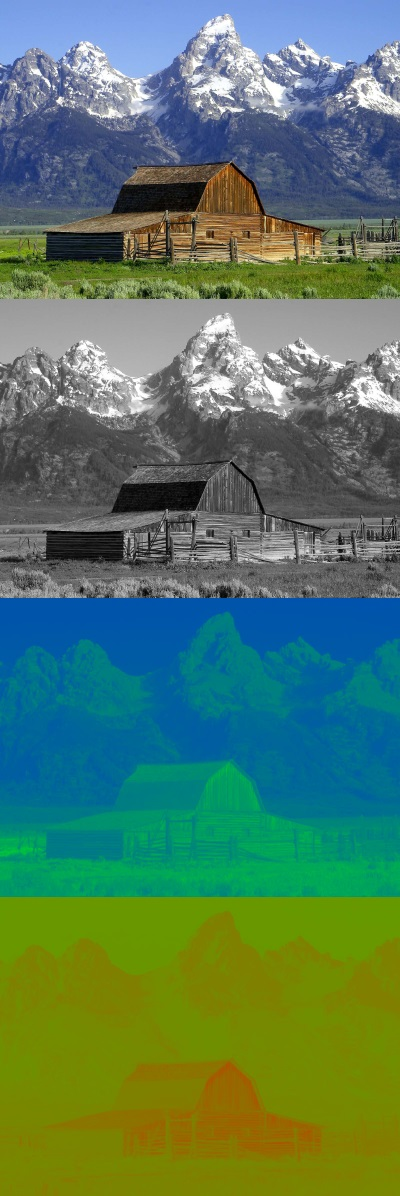
\includegraphics[totalheight=0.87\textheight,width=0.7\textwidth]{chapter2/yuv.jpg}
    \caption{Στην πρώτη εικόνα φαίνεται ένα καρέ με όλες τις συνιστώσες ενώ παρακάτω ξεχωριστά το YUV για το ίδιο καρέ \cite{wiki:yuv}.}
    \label{fig:yuv}
\end{figure}

\newpage
\section{Οργάνωση των pixels από τους κωδικοποιητές}
\label{section:sect23}

\indent Η πλειοψηφία των σημερινών κωδικοποιητών ομαδοποιούν τα pixels. Η πιο συνηθισμένη ομαδοποίηση είναι αυτή του macroblock, το κάθε καρέ διαιρείται σε μικρά πλακίδια σταθερής διάστασης NxN pixels όπου συνήθως N$=$16. Συνεπώς, το καρέ του παραδείγματος μας αποτελείται από $\frac{345600}{16*16} = 1350$ macroblocks που για YUV420 το καθένα περιέχει 1 Y macroblock 16x16 και 8 UV 8x8. Το κάθε macroblock μπορεί να σπάσει σε blocks και το κάθε block σε subblocks όπως φαίνεται στο Σχήμα~\ref{fig:mbpart}.

\begin{figure}[H]
  \centering
    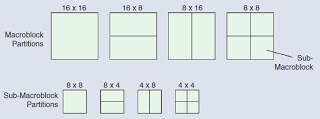
\includegraphics[width=0.7\textwidth]{chapter2/mbpart.jpg}
  \caption{Διαμερισμός του macroblock στον H.264.\cite{misc:mbpart}}
  \label{fig:mbpart}
\end{figure}

\indent Μετά τον χωρισμό σε macroblocks οι κωδικοποιητές ομαδοποιούν τα καρέ σε Intra και Inter (Temporal ή Special) με τα τελευταία να χωρίζονται σε P (predictive) και Β (bidirectional). Όλες οι παραπάνω κατηγοριοποιήσεις έχουν να κάνουν με τον μηχανισμό του Motion Estimation ο οποίος δημιουργεί διαφορές pixels (residuals). Κύριο χαρακτηριστικό των residuals είναι η μικρή τους ενέργεια (οι τιμές τους είναι κοντά στο 0).

\begin{itemize}
  \item Intra ή αλλιώς I είναι τα καρέ που χρησιμοποιούν πληροφορία μόνο από το τρέχον καρέ για να βγάλουν τα residuals. Αυτό γίνεται απλά παίρνοντας τις τιμές των γειτονικών block και εφαρμόζοντας ένα mode π.χ μέσος όρος όπου το αποτέλεσμα αυτού του mode αφαιρείται από τις τιμές των pixel του τρέχοντος block. Υπάρχουν διάφορα modes που μπορούν να γίνουν όπως φαίνεται και στο Σχήμα~\ref{fig:intrapred} και δοκιμάζονται κάθε φόρα όλα μέχρι να καταλήξουμε στο καλύτερο,δηλαδή αυτό που έχει το μικρότερο σφάλμα ή αυτό που χρειάζεται τον μικρότερο αριθμό από bits για να κωδικοποιηθεί. Η απόδοση της συμπίεσης είναι συγκριτικά η χειρότερη σε σχέση με τα άλλα είδη καρέ αλλά χωρίς αυτά το βίντεο δε θα μπορούσε να ξεκινήσει γιατί δεν θα υπήρχε σημείο εκκίνησης για να αποκωδικοποιηθεί η πληροφορία.

  \item P καρέ είναι αυτά τα οποία ψάχνουν το καλύτερο block για να κάνουν διαφορές από κάποιο αριθμό προηγούμενων καρέ όπως φαίνεται στο Σχήμα~\ref{fig:gop}. Επιπρόσθετα κάθε macroblock έχει ως pixel αναφοράς pixel που προέρχονται από ένα συγκεκριμένο καρέ.

  \item Β καρέ είναι αυτά τα οποία ψάχνουν το καλύτερο block για να κάνουν διαφορές από κάποιο αριθμό προηγούμενων αλλά και επόμενων καρέ όπως φαίνεται στο Σχήμα~\ref{fig:gop}. Σε αντίθεση με τα P τα macroblock των B μπορούν να προβλέπονται από τον μέσο όρο pixel που προέρχονται από δύο καρέ. Αυτά έχουν την καλύτερη απόδοση συμπίεσης αλλά η πολυπλοκότητα αποκωδικοποίησης είναι η μεγαλύτερη.
\end{itemize}

\indent Ένα επιπλέον στοιχείο των encoder είναι το group of pictures (GOP) το οποίο χαρακτηρίζει την σειρά με την οποία τα είδη των καρέ τοποθετούνται. Το GOP ξεκινάει από ένα I-frame συνεχίζει με P,B και περιοδικά έρχεται ένα I που σηματοδοτεί το τέλος του τρέχον GOP. Το GOP εξαρτάται από την εφαρμογή και μπορεί να έχει μεγάλες αποκλίσεις. Ένα τυπικό φαίνεται στο Σχήμα~\ref{fig:gop}

\indent Έτσι λοιπόν για να ανακατασκευαστεί ένα καρέ χρειάζεται την πληροφορία πρόβλεψης. Για τα Intra καρέ, αυτή η πληροφορία είναι το mode που έγινε η κωδικοποίηση Σχήμα~\ref{fig:intrapred}. Για τα Inter είναι ένα διάνυσμα τριών διαστάσεων (motion vector) $mv = [ framenum , x , y]$ ,  οπού $framenum$ είναι ο αριθμός του frame που βρίσκεται η πληροφορία και $x,y$ οι συντεταγμένες του. Εννοείται, πως το $framenum$, πρέπει ήδη να έχει αποκωδικοποιηθεί πλήρως είτε επειδή είναι Intra είτε επειδή έχει όλη την πληροφορία από προηγούμενα/επόμενα P,B καρέ.

\begin{figure}[H]
  \centering
    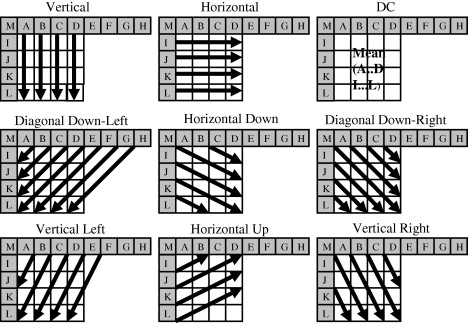
\includegraphics[width=0.7\textwidth]{chapter2/intrapred.jpg}
  \caption{Τρόποι που χρησιμοποιούνται στον Η.264 για Intra prediction. \cite{intrapred}}
    \label{fig:intrapred}
\end{figure}

\begin{figure}[H]
  \centering
    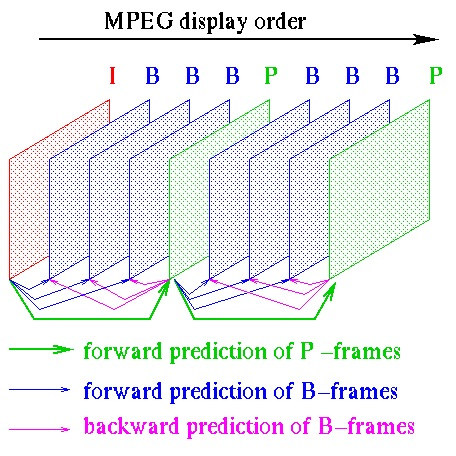
\includegraphics[width=0.7\textwidth]{chapter2/gop.jpg}
  \caption{Inter prediction στον mpeg και απεικόνιση ενός ενδεικτικού GOP. \cite{misc:gop}}
  \label{fig:gop}
\end{figure}

\newpage

\section{Μετασχηματισμός}
\label{section:sect24}

\indent Έχοντας ο encoder κατασκευάσει τα residuals για το macroblock, το επόμενο βήμα είναι ένας μετασχηματισμός, που συνήθως είναι ο διακριτός μετασχηματισμός συνημιτόνου DCT(Discrete Cosine Transform).Στους κωδικοποιητές mpeg1,2,4 εφαρμόζεται με διάσταση 8x8, στον H.264 και για 4x4 ενώ στον Η.265 και για 16x16. Αυτό συμβαίνει γιατί ο μετασχηματισμός επιστρέφει πολλά 0 αν το σήμα μας είναι χαμηλής ενέργειας, όπως συμβαίνει με τα residuals. Με αυτόν τον τρόπο, χρησιμοποιώντας κάποιο ειδικό σύμβολο μπορούν να απεικονιστούν πολλά μηδενικά του μετασχηματισμού και να μειωθεί το πλήθος των αριθμών προς κωδικοποίηση όπως φαίνεται στο Σχήμα~\ref{eq:rle} μέσω της εφαρμογής του αλγορίθμου RLE (Run Length Encoding). Η σάρωση του macroblock δεν γίνεται γραμμικά αλλά με την μέθοδο του zigzag όπως στο Σχήμα~\ref{fig:zigzag} γιατί έτσι έχει παρατηρηθεί πως έχουμε παραπάνω μηδενικά στην σειρά άρα και καλύτερη απόδοση του RLE.
\\
\\
\begin{figure}[H]
\centering
$
\begin{array}{| c | c | c | c | c | c | c | c | c | c |}
    \hline 17 & 8 & 54 & 0 & 0 & 0 & 97 & 5 & 0 & 16 \\ \hline
\end{array}
\xrightarrow[RLE]{}
\begin{array}{| c | c | c | c | c | c |}
    \hline (0,17) & (0,8) & (0,54) & (3,97) & (0,5) & (1,16) \\ \hline
\end{array}
$
\caption{Παραδείγμα χρήσης RLE}
\label{eq:rle}
\end{figure}

\begin{figure}[H]
  \centering
  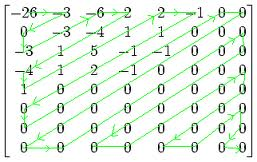
\includegraphics[width=0.7\textwidth]{chapter2/zigzag.jpg}
  \caption{Σάρωση ZigZag. \cite{misc:zigzag}}
  \label{fig:zigzag}
\end{figure}

\newpage
\section{Κβαντοποίηση}
\label{section:sect25}

\indent Η κβαντοποίηση είναι το σημείο που σε κάθε encoder εισάγεται το σφάλμα. Μετά τον μετασχηματισμό τα residuals έχουν αντικατασταθεί με συντελεστές οι οποίοι είναι πραγματικοί αριθμοί. Η τακτική που εφαρμόζεται είναι να γίνει ακέραια διαίρεση του συντελεστή της κάθε συχνότητας με έναν σταθερό ακέραιο αριθμό, πιθανόν διαφορετικό για κάθε συχνότητα όπως φαίνεται στον Πίνακα~\ref{table:quanttable}. Επομένως για τους δεδομένους πίνακες συντελεστών του Πίνακα~\ref{table:coeff} έχουμε τα αποτελέσματα στον Πίνακα~\ref{table:results} τα οποία είναι αυτά που θα δοθούν στο RLE και εν συνεχεία σε κάποιον entropy encoder για να συμπιεστούν.

\indent Ο Πίνακας~\ref{table:quanttable} μεταβάλλεται με βάση μια μεταβλητή που καθορίζει την ποιότητα του βίντεο η οποία ονομάζεται Quantization Parameter (QP). Στον H.264, το QP $\in [0,51] $. Στο περίπτωση του QP=0 εμφανίζεται η μέγιστη δυνατή ποιότητα η οποία μπορεί να θεωρηθεί σχεδόν χωρίς απώλειες (losless) και όσο το QP αυξάνει τόσο η ποιότητα πέφτει. Αυτό συμβαίνει γιατί το QP έχει αναλογική σχέση με τους πολλαπλασιαστές του Πίνακα~\ref{table:quanttable} του οποίου οι τιμές μεγαλώνουν. Επομένως, στην ακέραια διαίρεση χάνεται περισσότερο πληροφορία καθώς γίνεται διαίρεση με μεγαλύτερο αριθμό. Υπάρχει κέρδος όμως σε μέγεθος γιατί έτσι προκύπτουν περισσότερα μηδενικά και μικρότερες τιμές κατά απόλυτη τιμή οι οποίοι απαιτούν λιγότερα bits για την κωδικοποίηση τους.

\begin{table}[H]
    \begin{center}
        \begin{tabular}{| c  c  c  c  c  c  c  c |}
        \hline
        16 & 11 & 10 & 16 & 24 & 40 & 51 & 61 \\
        12 & 12 & 14 & 19 & 26 & 58 & 60 & 55 \\
        14 & 14 & 16 & 24 & 40 & 57 & 69 & 56 \\
        14 & 17 & 22 & 29 & 51 & 87 & 80 & 62 \\
        18 & 22 & 37 & 56 & 68 & 109 & 103 & 77 \\
        24 & 35 & 55 & 64 & 81 & 104 & 113 & 92 \\
        49 & 64 & 78 & 87 & 103 & 121 & 120 & 101 \\
        72 & 92 & 95 & 98 & 112 & 100 & 103 & 99 \\
        \hline
        \end{tabular}
    \end{center}
    \caption{Πίνακας Κβαντοποίησης. \cite{wiki:jpeg}}
    \label{table:quanttable}
\end{table}

\begin{table}[H]
    \begin{center}
        \begin{tabular}{| c  c  c  c  c  c  c  c |}
        \hline
        -415.38 & -30.19 & -61.20 & 27.24 & 56.13 & -20.10 & -2.39 & 0.46 \\
        4.47 & -21.86 & -60.76 & 10.25 & 13.15 & -7.09 & -8.54 & 4.88 \\
        -46.83 & 7.37 & 77.13 & -24.56 & -28.91 & 9.93 & 5.42 & -5.65 \\
        -48.53 & 12.07 & 34.10 & -14.76 & -10.24 & 6.30 & 1.83 & 1.95 \\
        12.12 & -6.55 & -13.20 & -3.95 & -1.88 & 1.75 & -2.79 & 3.14 \\
        -7.73 & 2.91 & 2.38 & -5.94 & -2.38 & 0.94 & 4.30 & 1.84 \\
        -1.03 & 0.18 & 0.42 & -2.42 & -0.88 & -3.02 & 4.12 & -0.66 \\
        -0.17 & 0.14 & -1.07 & -4.19 & -1.17 & -0.10 & 0.70 & 1.68 \\
        \hline
        \end{tabular}
    \end{center}
    \caption{Παράδειγμα συντελεστών DCT 8x8. \cite{wiki:jpeg}}
    \label{table:coeff}
\end{table}

\begin{table}[H]
    \begin{center}
        \begin{tabular}{| c  c  c  c  c  c  c  c |}
        \hline
        -26 & -3 & -6 & 2 & 2 & -1 & 0 & 0 \\
        0 & -2 & -4 & 1 & 1 & 0 & 0 & 0 \\
        -3 & 1 & 5 & -1 & -1 & 0 & 0 & 0 \\
        -3 & 1 & 2 & -1 & 0 & 0 & 0 & 0 \\
         1 & 0 & 0 & 0 & 0 & 0 & 0 & 0 \\
        0 & 0 & 0 & 0 & 0 & 0 & 0 & 0 \\
        0 & 0 & 0 & 0 & 0 & 0 & 0 & 0 \\
        0 & 0 & 0 & 0 & 0 & 0 & 0 & 0 \\
        \hline
        \end{tabular}
    \end{center}
    \caption{Κβαντοποιημένοι συντελεστές DCT. \cite{wiki:jpeg}}
    \label{table:results}
\end{table}

\section{Αποκωδικοποίηση βίντεο}
\label{section:sect26}

\indent Για την αποκωδικοποίηση εκτελούνται όλα τα βήματα που κάνει ο encoder με την ανάποδη σειρά.

\begin{itemize}
  \item Μετά την entropy decoding τα νούμερα πολλαπλασιάζονται με τα στοιχεία του πίνακα κβαντοποίησης. Έτσι ανακτώνται οι συντελεστές του μετασχηματισμού, έχοντας πλέον εισάγει το σφάλμα που προέκυψε λόγω της ακέραιας διαίρεσης και τοποθετούνται στη σωστή θέση του πίνακα με την αντίστροφη σάρωση zigzag.
  \item Γίνεται αντίστροφος μετασχηματισμός και ανακτώνται τα residuals.
  \item Τέλος το Motion Compensation βρίσκει τα ένα ή δύο blocks που χρησιμοποιήθηκαν για να παραχθούν τα residuals (μέσω των motion vectors) και τα προσθέτει με τα ανακατασκευασμένα residuals για να παραχθούν τα ανακατασκευασμένα pixels.
\end{itemize}

\section{Ποιότητα Βίντεο}
\label{section:sect27}

\indent Με τον όρο ποιότητα βίντεο ορίζουμε το μέσο όρο του αθροίσματος των διαφόρων στο τετράγωνο MSE (Mean Squared Error) όλων τον pixels μεταξύ του ασυμπίεστου βίντεο και του συμπιεσμένου. \begin{equation}
\text{MSE} =
\frac{\displaystyle\sum_{i=1}^{X*Y}
(Source_{pixel_i}-Reconstructed_{pixel_i})^{2}}{X*Y}
\end{equation}

\indent Συνήθως γίνεται μετατροπή του MSE σε PSNR (Peak Signal to Noise Ratio)  με μονάδα μέτρησης το \si{}{dB} με τον τύπο  $ PSNR = 10*\log_{10}{\frac{MAX_i^2}{MSE}}$ οπού το $MAX_i$ είναι η μέγιστη τιμή που μπορεί να πάρει ένα pixel. Αυτό εξαρτάται από το bitdepth, π.χ αν έχουμε bitdepth=8bits τότε $ MAX_i=255$.

\indent Ο μέσος όρος του PSNR όλων των καρέ μας δίνει την ποιότητα του βίντεο, το PSNR υπολογίζεται ξεχωριστά για τις συνιστώσες Y,UV και επειδή το ανθρώπινο μάτι είναι πιο ευαίσθητο στην φωτεινότητα, το Y λαμβάνεται ως μετρική για όλο το βίντεο.

\newpage

\section{Δομή του Η.264}
\label{section:sect28}

\indent Στο Σχήμα~\ref{fig:h264}, παρουσιάζεται η δομή του H.264 encoder. Το υποσύνολο με γκρι χρώμα είναι το κομμάτι του αποκωδικοποιητή (decoder). Κάθε encoder υλοποιεί στο εσωτερικό του και έναν decoder για να έχει τα pixel αναφοράς που χρησιμοποιούνται για το Motion Estimation και για το Motion Compensation συγχρονισμένα με τα αντίστοιχα pixel του αποκωδικοποιητή. Υπάρχουν και άλλα στοιχεία, όπως το φίλτρο απομάκρυνσης γραμμών (deblocking filter), ο ελεγκτής ρυθμού συμπίεσης (rate controller) που σε αυτή την διπλωματική δεν κρίνεται απαραίτητο να εξηγήθούν περαιτέρω διότι δεν βοηθούν στην κατανόηση της.

\begin{figure}[h]
    \centering
    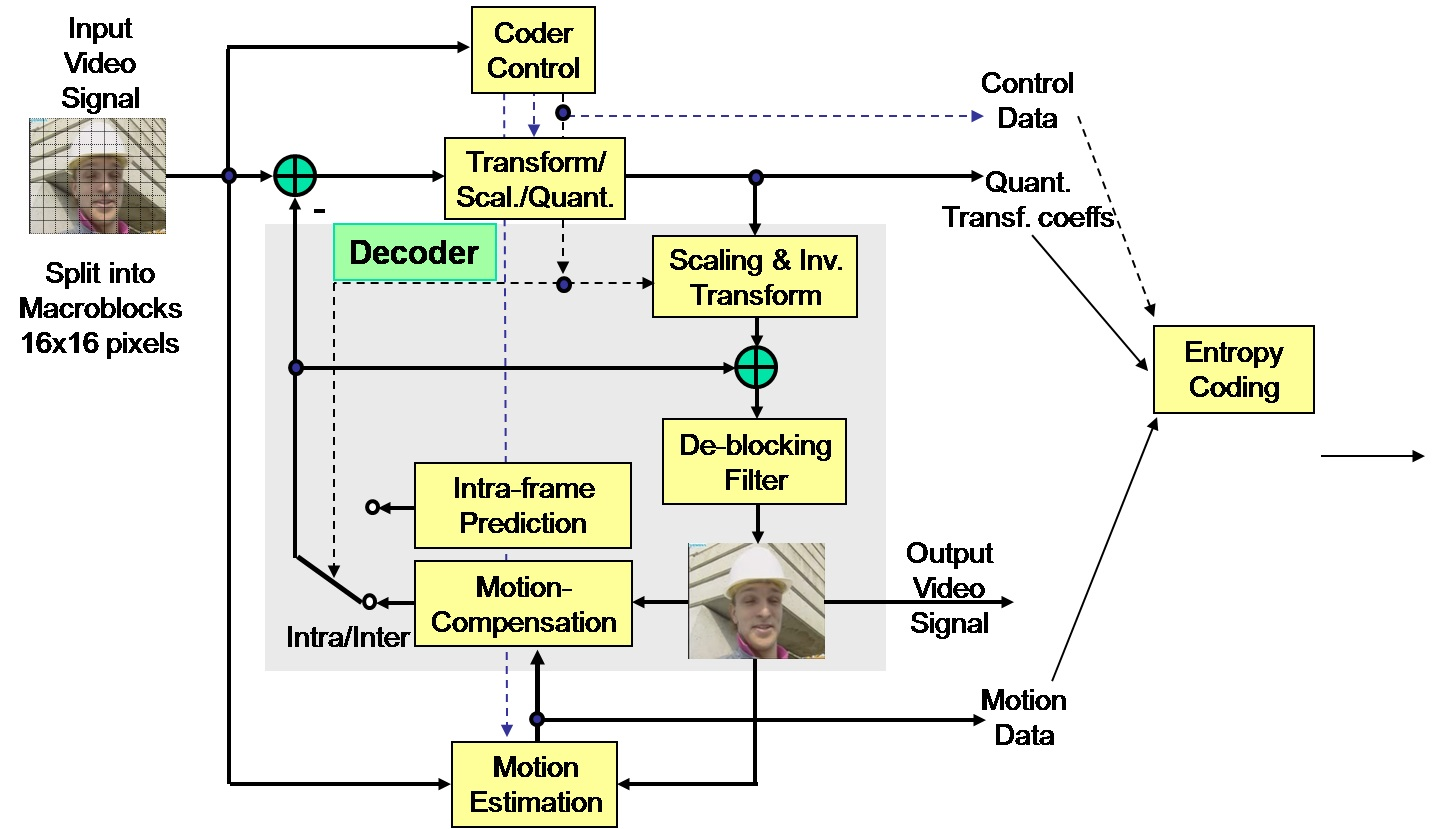
\includegraphics[width=0.7\textwidth]{chapter2/h264.jpg}
    \caption{H.264 encoder structure. \cite{misc:structure}}
    \label{fig:h264}
\end{figure}


%\chapter{Γενική Επισκόπηση του Επεξεργαστή Cell (Cell Broadband Engine)}
\label{chapter:chap3}

Στο παρόν κεφάλαιο γίνεται μία εισαγωγή στον επεξεργαστή \textsl{Cell}. Αρχικά, παρουσιάζονται τα κίνητρα για την δημιουργία του επεξεργαστή, έπειτα παρουσιάζεται η αρχιτεκτονική αυτού και τέλος αναλύονται τα εργαλεία για την ανάπτυξη εφαρμογών στον επεξεργαστή.

\section{Εισαγωγή}
\label{section:sect31}
\indent
Οι αυξανόμενες απαιτήσεις νέων εφαρμογών, όπως εφαρμογές πολυμέσων, σε υπολογιστική δύναμη έχουν οδηγήσει σε μία συνεχή αύξηση των απαιτήσεων για επεξεργαστική ισχύ.\newline \indent
Κατά την προηγούμενη δεκαετία, η έλευση της τεχνολογίας \ac{VLSI} και η συνεχής αλλαγή κλίμακας είχαν ως αποτέλεσμα την αύξηση της απόδοσης των μικροεπεξεργαστών κατά \(50\% - 60\%\). Οι κύριοι παράγοντες που συντελούσαν σε αυτή την αύξηση ήταν η αύξηση της ταχύτητας του ρολογιού, τόσο με την μείωση των επιπέδων λογικής για κάθε κύκλο ρολογιού όσο και με την αλλαγή κλίμακας της τεχνολογίας, όπως επίσης και η εκμετάλλευση του μεγάλου αριθμού των transistors σε κάθε chip, ο οποίος διπλασιαζόταν βάσει του \textsl{Νόμου του Moore}.\newline \indent
Πλέον, η επίτευξη μεγάλης απόδοσης στους μικροεπεξεργαστές με χρήση συμβατικών τεχνικών θα είναι πολύ δύσκολη. Ενώ η ταχύτητα των transistors αυξάνεται δραματικά, η ταχύτητα των καλωδίων μειώνεται. Σε συνδυασμό με την αύξηση του μεγέθους του chip, η οποία παρατηρείται στους νέους μικροεπεξεργαστές, ο χρόνος για να αποσταλεί ένα σήμα θα αυξηθεί σημαντικά αφού η απόσταση την οποία θα μπορεί το σήμα να διανύσει σε έναν κύκλο ρολογιού θα μειωθεί. Έτσι, δεν θα είναι δυνατή τόσο η αύξηση των σταδίων του pipeline, η οποία τα προηγούμενα χρόνια είχε επιφέρει σημαντική βελτίωση στην απόδοση των μικροεπεξεργαστών, όσο και η προσθήκη επιπλέον μονάδων εκτέλεσης καθώς η καθυστέρηση για την μετάδοση ενός σήματος μεταξύ των σταδίων του pipeline και μεταξύ των επιμέρους υπομονάδων θα αυξηθεί. Ο συνδυασμός των ανωτέρω θα έχει άμεση επίδραση στην διεκπεραιωτική ικανότητα (\textsl{throughput}) του επεξεργαστή.\newline \indent
Συν τοις άλλοις, η προαναφερθείσα αύξηση της καθυστέρησης θα αυξήσει και τον χρόνο που απαιτείται για πρόσβαση στις δομικές μονάδες του επεξεργαστή, όπως στους φακέλους καταχωρητών, στην μνήμη cache ακόμη και στο παράθυρο εντολών (\textsl{instruction window}). Καθώς η καθυστέρηση πρόσβασης εξαρτάται από την χωρητικότητα της κάθε μονάδας, για να είναι δυνατή η επίτευξη χαμηλής καθυστέρησης θα πρέπει η χωρητικότητα της κάθε μονάδας να μειωθεί. Αυτός θα είναι ένας παράγοντας που θα επηρεάσει την απόδοση των μικροεπεξεργαστών καθώς δεν θα είναι πλέον δυνατή η επίτευξη μεγαλύτερης απόδοσης μέσω της αύξησης του μεγέθους των δομικών μονάδων. Ως ενδεικτικό παράδειγμα μπορεί να αναφερθεί η εξάρτηση του παραλληλισμού που μπορεί να επιτευχθεί σε επίπεδο εντολής από το μέγεθος του παραθύρου εντολών.\newline \indent
Επίσης, η αύξηση της καθυστέρησης θα έχει άμεση επίδραση στον παραλληλισμό σε επίπεδο εντολών (ILP). Σε συνδυασμό με την αύξηση της συχνότητας του ρολογιού, η κατάσταση που θα μπορεί ο επεξεργαστής να εκμεταλλευτεί για δεδομένο βάθος του pipeline θα μειώνεται. Τέλος, η αύξηση της συχνότητας λειτουργίας του επεξεργαστή έχει ως αποτέλεσμα την αύξηση της καταναλισκόμενης ισχύος και ιδίως της στατικής συνιστώσας αυτής. Το κυρίως πρόβλημα που δημιουργεί η αύξηση της ισχύος είναι η αύξηση της πυκνότητας ισχύος, η οποία γίνεται εντονότερη με την αλλαγή κλίμακας των επεξεργαστών.\newline \indent
Λαμβάνοντας υπόψη τα ανωτέρω, οι σχεδιαστές μικροεπεξεργαστών στράφηκαν στην κατασκευή επεξεργαστών με μεγαλύτερο αριθμό από απλούστερους πυρήνες στο ίδιο \textsl{chip}. Αυτού του είδους οι επεξεργαστές αποκαλούνται επεξεργαστές πολλαπλών πυρήνων - \textsl{multicores}. Οι κυρίαρχες προσεγγίσεις στην  κατασκευή επεξεργαστών πολλαπλών πυρήνων είναι δύο. Η πρώτη είναι η \textsl{Συμμετρική Πολυεπεξεργασία} (\ac{SMP}), όπου σε ένα \textsl{chip} τοποθετούνται πολλαπλοί όμοιοι επεξεργαστές. Αυτή η προσέγγιση υιοθετείται από τις τελευταίες γενεές επεξεργαστών της \textsl{Intel} και της \textsl{AMD}. Η δεύτερη προσέγγιση συνίσταται στην δημιουργία \textsl{tiled} ή \textsl{heterogeneous} αρχιτεκτονικών. Χαρακτηριστικά παραδείγματα αυτής της προσέγγισης αποτελούν οι επεξεργαστές \textsl{Cell} \cite{Hofstee} και \textsl{RAW} \cite{Waingold, Taylor}.
\newline \indent
Ο επεξεργαστής \textsl{Cell} (\ac{CBE}) είναι ένας μικροεπεξεργαστής που δημιουργήθηκε από την συνεργασία των εταιρειών \textsl{Sony, Toshiba} και \textsl{IBM} το 2001 ώστε να αποτελέσει τον επεξεργαστή για την νέα \textsl{game console} της \textsl{Sony}, το \textsl{PlayStation 3}. Ενώ αρχικά σχεδιάστηκε για χρήση σε \textsl{game consoles} και σε συσκευές πολυμέσων για το καταναλωτικό κοινό, είναι αρκετά ευέλικτος ώστε να χρησιμοποιηθεί ως επεξεργαστής γενικού σκοπού. Ταυτόχρονα, υπάρχει μεγάλο ερευνητικό ενδιαφέρον για την χρήση του επεξεργαστή σε μία πληθώρα άλλων εφαρμογών όπως εφαρμογές επιστημονικού υπολογισμού ή εφαρμογές υπερ-υπολογισμού (\textsl{supercomputing}).\newline \indent
Η πρώτη υλοποίηση αυτού αποτελεί έναν \textsl{single-chip} επεξεργαστή πολλαπλών πυρήνων με εννέα επεξεργαστές, οι οποίοι λειτουργούν σε ένα μοντέλο κοινής μνήμης (\textsl{shared memory model}), όπως παρουσιάζεται στο σχήμα~\ref{figure:fig31}. Το χαρακτηριστικό που διαφοροποιεί τον \ac{CBE} από ήδη υπάρχοντες επεξεργαστές είναι ότι ενώ όλοι οι επεξεργαστές διαμοιράζονται την υπάρχουσα μνήμη, αυτοί ειδικεύονται σε δύο κατηγορίες: το \acf{PPE} και το \acf{SPE}. Ο επεξεργαστής \textsl{Cell} αποτελείται από έναν επεξεργαστή τύπου \ac{PPE} και οχτώ επεξεργαστές τύπου \ac{SPE}.

\begin{figure}
\centering
\includegraphics[width=5in, height=3in]{Chapter3/figures/figure1.eps}
\caption{Η αρχιτεκτονική του επεξεργαστή \textsl{Cell}.}
\label{figure:fig31}
\end{figure}
Ο πρώτος τύπος επεξεργαστικού στοιχείου, το \ac{PPE}, εμπεριέχει έναν πυρήνα \textsl{64-bit} PowerPC\circledR \ Architecture\(^{TM}\). Ο πυρήνας ακολουθεί την αρχιτεκτονική \textsl{64-bit} PowerPC και μπορεί να εκτελέσει λειτουργικά συστήματα και εφαρμογές \textsl{32-bit} και \textsl{64-bit}. Ο δεύτερος τύπος επεξεργαστικού στοιχείου, το \ac{SPE}, αποτελεί έναν πυρήνα βελτιστοποιημένο για την εκτέλεση \acf{SIMD} εφαρμογών με μεγάλες απαιτήσεις όσον αφορά στην επεξεργαστική ισχύ.\newline \indent
Τα \acp{SPE} είναι ανεξάρτητα επεξεργαστικά στοιχεία, με τον κάθε πυρήνα να εκτελεί τις δικές του εφαρμογές ή νήματα, και έχουν πλήρη πρόσβαση στην κοινή μνήμη. Μεταξύ των \acp{SPE} και του \ac{PPE} υπάρχει μία αμοιβαία εξάρτηση. Τα \acp{SPE} εξαρτώνται από το \ac{PPE} για την εκτέλεση του λειτουργικού συστήματος, την εκτέλεση διαφόρων κλήσεων συστήματος και στην πλειονότητα των περιπτώσεων για την εκτέλεση του νήματος που ελέγχει τα νήματα που εκτελούνται στα \acp{SPE}. Το \ac{PPE} εξαρτάται από τα \acp{SPE} τα οποία είναι υπεύθυνα για το μεγαλύτερο μέρος της απόδοσης του συστήματος.\newline \indent
Για τον προγραμματιστή κάποιας εφαρμογής, ο \textsl{Cell} αποτελεί έναν \textsl{dual-threaded} επεξεργαστή με οχτώ επιπλέον πυρήνες, οι οποίοι έχουν πρόσβαση στην δική τους τοπική μνήμη. Η ποικιλομορφία του \textsl{Cell}, με τον διαχωρισμό των πυρήνων σε πυρήνες βελτιστοποιημένους για λειτουργίες ελέγχου και πυρήνες βελτιστοποιημένους για υπολογισμούς, είναι το στοιχείο που επιτρέπει την δραματική βελτίωση στην μέγιστη υπολογιστική δυνατότητα που διαθέτει και τον καθιστά περισσότερο αποδοτικό, όσον αφορά στην κατανάλωση ισχύος και στην απαιτούμενη επιφάνεια για την υλοποίηση, έναντι συμβατικών μικροεπεξεργαστών.\newline \indent
Η κυριότερη διαφορά μεταξύ των δύο τύπων πυρήνων στον επεξεργαστή \textsl{Cell} είναι ο τρόπος με τον οποίο πραγματοποιείται η προσπέλαση μνήμης. Το μεν \ac{PPE} προσπελαύνει την κύρια μνήμη (\textsl{effective address space}) με εντολές τύπου \textsl{load, store}, με τα αποτελέσματα να αποθηκεύονται σε έναν ιδιωτικό φάκελο καταχωρητών ενώ δίνεται και η δυνατότητα για \textsl{caching} των δεδομένων. Αυτή η μέθοδος πρόσβασης ομοιάζει με τον τρόπο πρόσβασης στην μνήμη όπως αυτή πραγματοποιείται στους συμβατικούς μικροεπεξεργαστές.\newline \indent
Κάθε \ac{SPE}, σε αντίθεση, προσπελαύνει την κύρια μνήμη μέσω εντολών \acf{DMA}, οι οποίες μεταφέρουν δεδομένα μεταξύ της κύριας μνήμης και μίας τοπικής, ιδιωτικής, μνήμης, η οποία αποκαλείται \acf{LS}. Η τοπική μνήμη προσπελαύνεται απευθείας από τις εντολές προσκόμισης, φόρτωσης και αποθήκευσης ενώ δεν υπάρχει κάποια κρυφή μνήμη \textsl{cache}. Αυτή η ιεραρχία μνήμης τριών επιπέδων (φάκελος καταχωρητών, τοπική μνήμη, κύρια μνήμη), με τις ασύγχρονες εντολές \ac{DMA}, αποτελεί μία ριζική αλλαγή σε σχέση με τις συμβατικές αρχιτεκτονικές και τα προγραμματιστικά μοντέλα καθώς ο παραλληλισμός μεταξύ εκτέλεσης υπολογισμών και μεταφοράς δεδομένων είναι σαφής.\newline \indent
Το κυρίως κίνητρο για την υιοθέτηση αυτού του μοντέλου είναι η μεγάλη καθυστέρηση που υπάρχει για την προσπέλαση της κύριας μνήμης, η οποία έχει αυξηθεί δραματικά στις τελευταίες γενεές επεξεργαστών. Αυτό έχει σαν συνέπεια η απόδοση της εφαρμογής να εξαρτάται από την καθυστέρηση της μνήμης και όχι από την υπολογιστική ικανότητα. Επί παραδείγματι, εάν η εφαρμογή έχει μία αστοχία κατά την πρόσβαση στην μνήμη \textsl{cache}, θα πρέπει να παγώσει την εκτέλεσή της για αρκετούς κύκλους ρολογιού με αποτέλεσμα την μείωση της απόδοσης. Εν αντιθέσει, ο μικρός αριθμός κύκλων ρολογιού που απαιτείται για την έναρξη της εκτέλεσης μίας εντολής \ac{DMA} και η δυνατότητα επικάλυψης υπολογισμών και μεταφοράς δεδομένων με χρήση της τεχνικής του \textsl{multi-buffering} μπορούν να αυξήσουν την απόδοση της εκάστοτε εφαρμογής.\newline \indent
Με αυτόν τον καινοτόμο σχεδιασμό η μικρο-αρχιτεκτονική του επεξεργαστή \ac{CBEA} μπορεί να υποστηρίξει μεγάλη υπολογιστική ικανότητα μέσω της εκμετάλλευσης των παρακάτω:

\begin{itemize}

\item{\textsl{Παραλληλισμός μεταξύ των δεδομένων} (\ac{DLP}) με τις μονάδες \ac{SIMD} που βρίσκονται στα \acp{SPE}.}

\item{\textsl{Παραλληλισμός μεταξύ των εντολών} (\ac{ILP}) με την \textsl{dual-issue} αρχιτεκτονική των \textsl{pipelines}.}

\item{\textsl{Παραλληλισμός μεταξύ των νημάτων} (\ac{TLP}) μέσω των πολλαπλών \acp{SPU}.}

\end{itemize}
\indent
Επίσης, η σχεδίαση του συστήματος της μνήμης παρέχει έναν μεγάλο βαθμό από ταυτόχρονες μεταφορές δεδομένων, οι οποίες πραγματοποιούνται υπό τον έλεγχο της εφαρμογής για την υποστήριξη μεγαλύτερης απόδοσης του συστήματος μνήμης. Με αυτά τα χαρακτηριστικά, η εκάστοτε εφαρμογή μπορεί να έχει τον πλήρη έλεγχο των διαθέσιμων πόρων της αρχιτεκτονικής ώστε να επιτευχθεί η μέγιστη δυνατή απόδοση.

\subsection[3.1.1 Αντιμετώπιση των κύριων περιοριστικών παραγόντων της απόδοσης]{Αντιμετώπιση των κύριων περιοριστικών παραγόντων της απόδοσης}
\label{subsection:sub311}
\indent
Η απόδοση των σύγχρονων επεξεργαστών καθορίζεται από τρεις σημαντικούς παράγοντες: την συχνότητα λειτουργίας, την καθυστέρηση πρόσβασης στην μνήμη και την καταναλισκόμενη ισχύ. Αυτοί οι παράγοντες συχνά αναφέρονται και ως \textsl{frequency wall, memory wall} και \textsl{power wall}. Η αρχιτεκτονική του \textsl{Cell} είναι τέτοια ώστε να αντιμετωπίζει επιτυχώς αυτούς του παράγοντες.\newline \indent

\subsubsection{Frequency Wall}
\label{subsubsection:subsub3111}
\indent
Οι συμβατικοί επεξεργαστές απαιτούν την αύξηση του βάθους του \textsl{pipeline} ώστε να επιτύχουν υψηλές συχνότητες λειτουργίας και να αυξήσουν την απόδοσή τους. Όμως, η τεχνική αυτή έχει φθάσει στο σημείο όπου επιπλέον αύξηση οδηγεί σε μειούμενα οφέλη (\textsl{law of diminishing effects}) - ακόμη και σε αρνητικές επιπτώσεις σε περίπτωση που η κατανάλωση ισχύος ληφθεί υπόψη.\newline \indent
Εξειδικεύοντας την λειτουργία του \ac{PPE} και του \ac{SPE} για εργασίες όπου κυριαρχούν οι εντολές ελέγχου (\textsl{control-intensive tasks}) και για εργασίες όπου κυριαρχούν οι εντολές υπολογισμού (\textsl{data-intensive tasks}) αντίστοιχα, η αρχιτεκτονική στην οποία βασίζεται ο \textsl{Cell} επιτρέπει τον αποδοτικό σχεδιασμό αυτών των στοιχείων για λειτουργία σε υψηλές συχνότητες χωρίς υπερβολική επιβάρυνση.\newline \indent
Το \ac{PPE} επιτυγχάνει υψηλή αποδοτικότητα βελτιστοποιώντας την εκτέλεση και των δύο διαθέσιμων νημάτων, αντί ενός, ενώ το \ac{SPE} επιτυγχάνει υψηλή αποδοτικότητα με χρήση του μεγάλου φακέλου καταχωρητών, ο οποίος επιτρέπει την ταυτόχρονη εκτέλεση αρκετών εντολών χωρίς την επιβάρυνση από τεχνικές όπως \textsl{register renaming} ή \textsl{out-of-order execution}. Επίσης, η χρήση των ασύγχρονων εντολών \ac{DMA} επιτρέπει την πρόσβαση στην μνήμη πολλαπλών εντολών χωρίς την επιβάρυνση από τον μηχανισμό του \textsl{speculation} που υπάρχει στους συμβατικούς, σύγχρονους επεξεργαστές.

\subsubsection{Memory Wall}
\label{subsubsection:subsub3112}
\indent
Οι σύγχρονοι πολυ-επεξεργαστές χαρακτηρίζονται από την μεγάλη καθυστέρηση για την πρόσβαση στην κύρια μνήμη, η οποία προσεγγίζει την τιμή των χιλίων κύκλων μηχανής. Αυτό έχει ως αποτέλεσμα, η απόδοση των εφαρμογών να εξαρτάται από την μεταφορά δεδομένων από και προς την κύρια μνήμη. Η αντιδραστική, \textsl{reactive}, φύση της κρυφής μνήμης δεν επιφέρει κάποια βελτίωση και πλέον ο μεταγλωττιστής, ή ακόμη και ο προγραμματιστής της εφαρμογής, επιφορτίζεται με την ρητή μεταφορά των δεδομένων.\newline \indent
Για την αντιμετώπιση αυτής της καθυστέρησης, τα \acp{SPE} του επεξεργαστή \textsl{Cell} υιοθετούν δύο τεχνικές:

\begin{itemize}

\item{Ιεραρχία μνήμης τριών επιπέδων (φάκελος καταχωρητών, τοπική μνήμη, κύρια μνήμη)}

\item{Ασύγχρονες εντολές \ac{DMA}}

\end{itemize}
\indent
Αυτοί οι μηχανισμοί επιτρέπουν στον προγραμματιστή της εφαρμογής να επικαλύψει την καθυστέρηση πρόσβασης στην κύρια μνήμη με την ταυτόχρονη δρομολόγηση υπολογισμών και μεταφοράς δεδομένων. Ενδεικτικά αναφέρεται ότι είναι δυνατή η υποστήριξη 128 ταυτόχρονων μεταφορών, αριθμός ο οποίος υπερβαίνει τον αριθμό των ταυτόχρονων μεταφορών που υποστηρίζονται από τους συμβατικούς επεξεργαστές κατά έναν παράγοντα ίσο με είκοσι.

\subsubsection{Power-limitation Wall}
\label{subsubsection:subsub3113}
\indent
Η απόδοση των μικροεπεξεργαστών εξαρτάται σε μεγάλο βαθμό από την κατανάλωση ισχύος και όχι από τους διαθέσιμους πόρους, όπως \textsl{transistors} και καλωδιώσεις. Επομένως, ο μόνος τρόπος για την αύξηση της απόδοσης είναι η αύξηση της αποδοτικότητας στην κατανάλωση ισχύος με την ταυτόχρονη αύξηση της συχνότητας λειτουργίας.\newline \indent
Μία μέθοδος για την επίτευξη αποδοτικότητας στην κατανάλωση ισχύος είναι ο διαχωρισμός μεταξύ επεξεργαστών που είναι βελτιστοποιημένοι για την εκτέλεση \textsl{control-intensive tasks} και επεξεργαστών που είναι βελτιστοποιημένοι για την εκτέλεση \textsl{data-intensive tasks}.\newline \indent
Όπως αναφέρθηκε και παραπάνω, ο επεξεργαστής \textsl{Cell} διαθέτει έναν επεξεργαστή, το \ac{PPE}, βελτιστοποιημένο για την εκτέλεση του λειτουργικού συστήματος και την εκτέλεση \textsl{control-intensive} λειτουργιών και οχτώ επεξεργαστές, τα \acp{SPE}, για την εκτέλεση \textsl{data-intensive} λειτουργιών. Η αρχιτεκτονική των \acp{SPE} είναι αρκετά απλή καθώς δεν υπάρχουν μηχανισμοί όπως \textsl{branch prediction, out-of-order execution, speculative execution} και \textsl{register renaming}, οι οποίοι υπάρχουν σε άλλους σύγχρονους επεξεργαστές και συμβάλλουν στην επιτάχυνση της εκτέλεσης των προγραμμάτων. Επομένως, ο αριθμός των \textsl{transistors} που εξοικονομείται από την απουσία αυτών αφιερώνεται για την εκτέλεση υπολογισμών καθιστώντας τα \acp{SPE} πολύ αποδοτικά.

\section{Η Αρχιτεκτονική του Επεξεργαστή Cell}
\label{section:sect32}
\indent
Το πρώτο πρωτότυπο του \textsl{Cell} ήταν υλοποιημένο σε τεχνολογία \textsl{90nm SOI}, αποτελούνταν από 234 εκατομμύρια \textsl{transistors}, είχε κατανάλωση ίση με 60-80 \textsl{W} και τάση τροφοδοσίας ίση με 1.1 \textsl{V} ενώ λειτουργούσε σε συχνότητα ίση με \textsl{3.2 GHz}. Η υλοποίηση του πρωτοτύπου παρουσιάζεται στο σχήμα~\ref{figure:fig32} \cite{CellProject} ενώ ένα ενδεικτικό σχήμα για την δομή του \textsl{Cell} παρουσιάζεται στο σχήμα~\ref{figure:fig33}.
\begin{figure}[b]
\centering
\includegraphics[width=2in, height=3in]{Chapter3/figures/figure2.eps}
\caption{Εικόνα από ένα chip του επεξεργαστή \textsl{Cell}.}
\label{figure:fig32}
\end{figure}

\begin{figure}[b]
\centering
\includegraphics[width=5in, height=3in]{Chapter3/figures/figure3.eps}
\caption{Δομικό διάγραμμα του επεξεργαστή \textsl{Cell}.}
\label{figure:fig33}
\end{figure}

\subsection[3.2.1 Power Processing Element (PPE)]{Power Processing Element (PPE)}
\label{subsection:sub321}
\indent
Το \acf{PPE}, όπως υποδηλώνει και το όνομα αυτού, αποτελεί έναν επεξεργαστή \ac{RISC} που υποστηρίζει την \textsl{64-bit} αρχιτεκτονική \textsl{PowerPC} με τις \ac{SIMD} επεκτάσεις αυτές, γνωστές και ως επεκτάσεις \textsl{AltiVec}. Το \ac{PPE} υποστηρίζει την ταυτόχρονη εκτέλεση δύο νημάτων, επιτρέποντας έτσι την ταυτόχρονη διεκπεραίωση δύο λειτουργιών. Στον επεξεργαστή \textsl{Cell}, το \ac{PPE} εκτελεί το λειτουργικό σύστημα και, στην πλειονότητα των περιπτώσεων, εκτελεί και τον κώδικα που ελέγχει και συντονίζει την λειτουργία των \acp{SPE}. Το σχήμα~\ref{figure:fig34} παρουσιάζει την αρχιτεκτονική του \ac{PPE}.

%\begin{figure}[t]
%\centering
%\includegraphics[width=5in, height=3in]{Chapter3/figures/figure4.eps}
%\caption{Δομικό διάγραμμα του \textsl{PPE}.}
%\label{figure:fig34}
%\end{figure}
\indent
Οι κύριες υπομονάδες που αποτελούν το \ac{PPE} είναι η μονάδα \acf{PPU} και το υποσύστημα \acf{PPSS}, το οποίο αποτελεί το υποσύστημα για την διαχείριση της μνήμης. Η μονάδα \ac{PPU} αποτελείται από τις ακόλουθες επιμέρους μονάδες:

\begin{itemize}

\item{\acf{IU}: Αυτή η υπομονάδα εκτελεί την προσκόμιση και την αποκωδικοποίηση των εντολών. Έπειτα, κατευθύνει αυτές στην κατάλληλη υπομονάδα για την εκτέλεση της εντολής. Εμπεριέχει την υπομονάδα \acf{BRU} και μία κρυφή μνήμη εντολών (\textsl{L1 instruction cache}) μεγέθους \(32KB\).}

\item{\acf{LSU}: Η υπομονάδα \ac{LSU} λαμβάνει αιτήσεις από την μνήμη, τις οποίες προωθεί στο υποσύστημα \ac{PPSS} και εμπεριέχει μία κρυφή μνήμη δεδομένων (\textsl{L1 data cache}) μεγέθους \(32KB\).}

\item{\acf{VSU}: Αυτή η υπομονάδα περιλαμβάνει την μονάδα \acf{FPU}, η οποία εκτελεί πράξεις σε βαθμωτές μεταβλητές ακεραίων κινητής υποδιαστολής, και την μονάδα \acf{VXU}, η οποία εκτελεί πράξεις σε διανύσματα (\textsl{vectors}) τύπου ακεραίων κινητής υποδιαστολής. Τα διανύσματα είναι μεγέθους \(128-bits\) και σε αυτή την μονάδα εκτελούνται και οι πράξεις που ορίζονται από τις επεκτάσεις \textsl{Vector/SIMD Multimedia Extensions (AltiVec)}.}

\item{\acf{FXU}: Η υπομονάδα \ac{FXU} εκτελεί πράξεις σε ακεραίους όπως λογικές ή αριθμητικές πράξεις.}

\item{\acf{MMU}: Η υπομονάδα \ac{MMU} διαχειρίζεται το σύστημα εικονικής μνήμης του \textsl{Cell} και είναι υπεύθυνη για την μετάφραση των \textsl{ενεργών διευθύνσεων} (\textsl{effective addresses}) σε \textsl{εικονικές} και \textsl{πραγματικές διευθύνσεις}.}

\item{\acf{BRU}: Η υπομονάδα \ac{BRU} επεξεργάζεται τις εντολές διακλαδώσεων που υπάρχουν στο κώδικα της εκάστοτε εφαρμογής.}

\end{itemize}
\indent
Η ιεραρχία κρυφής μνήμης του \ac{PPE} αποτελείται από μία \textsl{Level-1} κρυφή μνήμη εντολών, με μέγεθος ίσο με \(32\ KB\), μία \textsl{Level-1} κρυφή μνήμη δεδομένων με μέγεθος ίσο με \(32\ KB\), και μία ενοποιημένη \textsl{Level-2 write-back} μνήμη εντολών και δεδομένων με μέγεθος ίσο με \(512\ KB\). Οι δύο \textsl{Level-1} μνήμες υποστηρίζουν συνεκτική πρόσβαση στα δεδομένα, με κάθε φόρτωση να έχει μέγεθος ίσο με \(16\) ή \(32\) bytes.\newline \indent
Η αρχιτεκτονική του \ac{PPE} υποστηρίζει το σύνολο εντολών της αρχιτεκτονικής \textsl{PPC 970} και το πλήρες σύνολο των εντολών \textsl{AltiVec/VMX}. Όπως κάθε αρχιτεκτονική τύπου \textsl{RISC}, η πλειονότητα των εντολών εκτελούν πράξεις μεταξύ καταχωρητών ενώ συγκεκριμένες εντολές χρησιμοποιούνται για πρόσβαση στην μνήμη.\newline \indent
Επίσης, υποστηρίζεται ένα μικρό σύνολο διαφορετικών κωδικοποιήσεων για τις διαθέσιμες εντολές ενώ όλες οι διαφορετικές κωδικοποιήσεις έχουν το ίδιο μέγεθος. Το σύνολο καταχωρητών που είναι διαθέσιμο στον προγραμματιστή αποτελείται από 32 καταχωρητές γενικού σκοπού με μέγεθος ίσο με \(64\ bits\), 32 καταχωρητές με μέγεθος ίσο με \(64\ bits\) για την αποθήκευση αριθμών κινητής υποδιαστολής που ακολουθούν το πρότυπο \textsl{IEEE-754} και 32 διανυσματικούς καταχωρητές μεγέθους ίσο με \(128\ bits\) για την αποθήκευση δεδομένων που χρησιμοποιούνται σε διανυσματικές πράξεις.\newline \indent
Όπως αναφέρθηκε παραπάνω και παρουσιάζεται και στο σχήμα~\ref{figure:fig34}, το \ac{PPE} αποτελεί έναν επεξεργαστή \textsl{RISC}, με δύο \textsl{hardware threads} ενώ δεν υποστηρίζεται η εκτέλεση εντολών εκτός σειράς. Σε κάθε κύκλο ρολογιού εισέρχονται προς επεξεργασία δύο εντολές, οι οποίες κατευθύνονται προς την κατάλληλη υπομονάδα εκτέλεσης όπως αυτή καθορίζεται από την υπομονάδα \ac{IU}. Σε περίπτωση που δεν υπάρχουν εξαρτήσεις μεταξύ των εντολών, αυτές εκτελούνται παράλληλα οπότε αυξάνεται η ικανότητα διεκπεραίωσης του επεξεργαστή. Επίσης, κατά την φάση της αποκωδικοποίησης ελέγχεται κατά πόσο η τρέχουσα εντολή αποτελεί μία \textsl{microcoded} εντολή. Η εκτέλεση τέτοιου είδους εντολών απαιτεί τον διαχωρισμό αυτών σε επιμέρους, απλούστερες εντολές. Γι' αυτό το στάδιο απαιτούνται 11 κύκλοι ρολογιού οπότε οι \textsl{microcoded} εντολές θα πρέπει να αποφεύγονται λόγω της μεγάλης καθυστέρησης που εισάγουν.\newline \indent
Τέλος, ένα σημαντικό τμήμα της αρχιτεκτονικής κάθε επεξεργαστή είναι η πρόβλεψη διακλαδώσεων (\textsl{branch prediction}) λόγω της μεγάλης καθυστέρησης που εισάγει μία λανθασμένη πρόβλεψη, η οποία ανέρχεται σε 23 κύκλους ρολογιού λόγω της επιβάρυνσης που εισάγεται από την διαδικασία αδειάσματος (\textsl{flushing}) του \textsl{pipeline}. Το \ac{PPE} υλοποιεί την πρόβλεψη διακλαδώσεων όπως ορίζεται από την αρχιτεκτονική \textsl{PPC 970}. Η αρχιτεκτονική συνόλου εντολών του \textsl{PowerPC} εμπεριέχει μία πληθώρα εντολών διακλάδωσης, πολλές από τις οποίες χρησιμοποιούνται ώστε να παρέχουν υποδείξεις στην υπομονάδα \ac{IU} ως προς το ποιο είναι το πιο πιθανό αποτέλεσμα της διακλάδωσης. Ένα χαρακτηριστικό παράδειγμα εντολής υψηλού επιπέδου είναι η εντολή \textsl{\_\_builtin\_expect}. Αυτού του είδους οι εντολές αναγνωρίζονται από τους αντίστοιχους μεταγλωττιστές οι οποίοι εισάγουν τις κατάλληλες εντολές \textsl{assembly}.
\begin{figure}[t]
\centering
\includegraphics[width=5in, height=3in]{Chapter3/figures/figure4.eps}
\caption{Δομικό διάγραμμα του \textsl{PPE}.}
\label{figure:fig34}
\end{figure}
\newline \indent
Όσον αφορά στον προγραμματισμό του \ac{PPE}, αυτός πραγματοποιείται χρησιμοποιώντας τις υψηλού επιπέδου γλώσσες \textsl{C/C++} ενώ παρέχεται και ένα σύνολο εσωτερικών εντολών\footnote{\small Οι εντολές αυτές ονομάζονται \textsl{intrinsics} και αντιστοιχούν σε μία ή περισσότερες εντολές \textsl{assembly}.}, όπως για παράδειγμα αυτές που υλοποιούν τις επεκτάσεις \textsl{AltiVec/VMX}.

\subsection[3.2.2 Synergistic Processing Element (SPE)]{Synergistic Processing Element (SPE)}
\label{subsection:sub322}
\indent
Παρόλη την υπολογιστική δύναμη του \ac{PPE}, η ασυνήθης υπολογιστική δύναμη του επεξεργαστή \textsl{Cell} πηγάζει από το \acf{SPE}. Σε αντίθεση με την αρχιτεκτονική γενικού σκοπού του \ac{PPE}, η αρχιτεκτονική του \ac{SPE} σχεδιάστηκε με κύριο γνώμονα την εκτέλεση διανυσματικών υπολογισμών με πολύ μεγάλη ταχύτητα. Το \textsl{datapath} της αρχιτεκτονικής έχει εύρος ίσο με \(128\ bits\) ενώ το \textsl{pipeline} είναι \textsl{dual-issue}, δηλαδή υποστηρίζεται η εκτέλεση δύο εντολών σε κάθε κύκλο ρολογιού. Όμως, η εκτέλεση δύο εντολών είναι δυνατή μόνο στην περίπτωση που δεν υπάρχουν εξαρτήσεις μεταξύ αυτών ενώ σε κάθε \textsl{pipeline} εκτελούνται εντολές από συγκεκριμένες κλάσεις εντολών. Καθένα από τα οχτώ \acp{SPE} αποτελείται από την υπομονάδα \ac{SPU} και τον \textsl{ελεγκτή ροής μνήμης} (\ac{MFC}). Το δομικό διάγραμμα του \ac{SPE} όπως επίσης και τα στάδια του \textsl{pipeline} για κάθε μία από τις διαθέσιμες κλάσεις εντολών παρουσιάζονται στο σχήμα~\ref{figure:fig35}.

\begin{figure}
\centering
\includegraphics[width=5in, height=4in]{Chapter3/figures/figure5.eps}
\caption{Δομικό διάγραμμα του \textsl{SPE}.}
\label{figure:fig35}
\end{figure}
\indent
Οι κύριες υπομονάδες που αποτελούν κάθε \ac{SPE} είναι οι ακόλουθες:

\begin{itemize}

\item{SPU Control Unit (SCN): Η μονάδα αυτή προσκομίζει και διανέμει τις εντολές στις αντίστοιχες μονάδες εκτέλεσης εντολών. Επίσης εκτελεί τις διάφορες εντολές ελέγχου, όπως για παράδειγμα εντολές διακλαδώσεων.}

\item{SPU Even Fixed-Point Unit (SFX): Σε αυτή την μονάδα εκτελούνται λογικές και αριθμητικές εντολές, εντολές σύγκρισης όπως επίσης και εντολές για αντιστροφή αριθμών κινητής υποδιαστολής.}

\item{SPU Odd Fixed-Point Unit (SFS): Η μονάδα αυτή είναι υπεύθυνη για την εκτέλεση πράξεων ολίσθησης, περιστροφής και ανακατέματος (\textsl{shuffling}).}

\item{SPU Floating-Point Unit (SFP): Στην εν λόγω μονάδα εκτελούνται οι αριθμητικές πράξεις σε ακεραίους κινητής υποδιαστολής, απλής ή διπλής ακρίβειας, πράξεις πολλαπλασιασμού ακεραίων όπως επίσης και διάφορες πράξεις μετατροπής ακεραίων.}

\item{SPU Load/Store Unit (SLS): Η μονάδα \textsl{SLS} είναι υπεύθυνη για την διαχείριση των διαφόρων εντολών που αφορούν στην μνήμη. Εδώ εκτελούνται εντολές φόρτωσης και αποθήκευσης στην τοπική μνήμη όπως επίσης και εντολές για αιτήσεις \ac{DMA} στην τοπική μνήμη.}

\item{SPU Channel and DMA Unit (SSC): Αυτή η μονάδα εκτελεί τις διάφορες λειτουργίες επικοινωνίας με τον \textsl{ελεγκτή ροής μνήμης} (\ac{MFC}) και διαχειρίζεται τις μεταφορές δεδομένων μέσω του μηχανισμού \ac{DMA}.}

\end{itemize}
\begin{table}
\centering
\begin{tabular}{|c|c|c|}
  \hline
  Τύπος Δεδομένων & Περιεχόμενα Τύπου Δεδομένων & Μέγεθος (bytes) \\ \hline
  boolean & True/False & 1 \\ \hline
  char & Χαρακτήρας ASCII & 1 \\ \hline
  unsigned char & Ακέραιος (0-255) & 1 \\ \hline
  short & Προσημασμένος ακέραιος τύπου short & 2 \\ \hline
  unsigned short & Μη προσημασμένος ακέραιος τύπου short & 2 \\ \hline
  int & Προσημασμένος Ακέραιος & 4 \\ \hline
  unsigned int & Μη προσημασμένος ακέραιος & 4 \\ \hline
  float & Ακέραιος κινητής υποδιαστολής, απλής ακρίβειας & 4 \\ \hline
  double & Ακέραιος κινητής υποδιαστολής, διπλής ακρίβειας & 8 \\ \hline
  long long / long long int & Προσημασμένος ακέραιος τύπου long long & 8 \\ \hline
  unsigned long long / & & \\
  unsigned long long int & Μη προσημασμένος ακέραιος τύπου long long & 8 \\ \hline
  qword & Εξαρτώνται από την εντολή & 16 \\
  \hline
\end{tabular}
\caption{Τύποι δεδομένων βαθμωτών μεταβλητών στα \textsl{SPUs}}
\label{table:tab31}
\end{table}
\indent
Τα χαρακτηριστικά που διαφοροποιούν την αρχιτεκτονική του \ac{SPE} από την αρχιτεκτονική του \ac{PPE} είναι η απουσία κρυφής μνήμης (\textsl{cache hierarchy}) και εικονικής μνήμης, η απουσία μονάδων που επεξεργάζονται βαθμωτές μεταβλητές, καθώς όλες οι πράξεις πραγματοποιούνται σε διανύσματα, και τα δύο διαφορετικά \textsl{pipelines}.\newline \indent
Κάθε \ac{SPE} αποτελείται από μία τοπική μνήμη, αποκλειστικής πρόσβασης και μεγέθους \(256\ KB\) (\ac{LS}), η οποία είναι οργανωμένη σε τέσσερεις \textsl{SRAM arrays} μεγέθους \(64\ KB\). Η μνήμη έχει μόνο μία θύρα ανάγνωσης/εγγραφής και γι' αυτό οι λειτουργίες πρόσβασης σε αυτή είναι \textsl{fully pipelined} ώστε να επιτυγχάνεται ταχύτερη πρόσβαση σε αυτή. Το εύρος ζώνης της μνήμης είναι ίσο με \(16\ bytes\) ανά κύκλο ενώ εντολές τύπου \textsl{DMA} μεταφέρουν από και προς την μνήμη δεδομένα που είναι οργανωμένα σε μονάδες μεγέθους \(1024\ bytes\).\newline \indent
Ένα ιδιαίτερο χαρακτηριστικό της μνήμης είναι ότι η πρόσβαση σε αυτή ξεκινά από διευθύνσεις που είναι πολλαπλάσιες των \(16\ bytes\) (quadword alignment). Σε περίπτωση που αυτό δεν ισχύει, εκτελούνται επιπλέον πράξεις για την ικανοποίηση των περιορισμών ευθυγράμμισης. Όπως είναι εμφανές, για την ικανοποίηση των περιορισμών πρέπει να ληφθεί ειδική μέριμνα από τον προγραμματιστή της εφαρμογής προκειμένου να μην επιβαρύνεται η εκτέλεση της εφαρμογής με το κόστος που συνεπάγονται οι προαναφερθείσες πράξεις ευθυγράμμισης. \newline \indent
Καθώς η μνήμη έχει μόνο μία θύρα εγγραφής/ανάγνωσης, όλες οι εντολές προσπέλασης στην μνήμη, όπως εντολές φόρτωσης και αποθήκευσης, συναγωνίζονται για την πρόσβαση σε αυτή την θύρα. Για την επίλυση αυτών των συγκρούσεων, επιβάλλεται ένα σχήμα προτεραιοτήτων μεταξύ αυτών των εντολών. Οι εντολές του μηχανισμού \ac{DMA} έχουν την μεγαλύτερη προτεραιότητα, μετά ακολουθούν οι εντολές φόρτωσης και αποθήκευσης ενώ την χαμηλότερη προτεραιότητα έχουν οι προσπελάσεις για την προσκόμιση εντολών.\newline \indent
Ο φάκελος καταχωρητών σε κάθε \ac{SPE} έχει μέγεθος ίσο με 128 καταχωρητές, όπου κάθε καταχωρητής έχει μήκος ίσο με \(128\ bits\). Οι διαθέσιμοι τύποι δεδομένων για τις βαθμωτές μεταβλητές και τις διανυσματικές μεταβλητές σε κάθε \ac{SPU}, όπως επίσης και το μέγεθος αυτών αναφέρονται στους πίνακες~\ref{table:tab31} και~\ref{table:tab32}.
\begin{table}
\centering
\begin{tabular}{|c|c|}
  \hline
  Διανυσματικός Τύπος Δεδομένων & Πλήθος Στοιχείων του Καταχωρητή \\ \hline
  vector unsigned char & 16 μη προσημασμένοι χαρακτήρες, \\
                       & μεγέθους 8-bit \\ \hline
  vector signed char & 16 προσημασμένοι χαρακτήρες, \\
                     & μεγέθους 8-bit \\ \hline
  vector unsigned short & 8 μη προσημασμένοι ακέραιοι τύπου short, \\
                        & μεγέθους 16-bit \\ \hline
  vector signed short & 8 προσημασμένοι ακέραιοι τύπου short, \\
                      & μεγέθους 16-bit \\ \hline
  vector pixel & 8 μη προσημασμένες μεταβλητές τύπου halfword, \\
               & μεγέθους 16-bit \\ \hline
  vector unsigned int & 4 μη προσημασμένοι ακέραιοι \\ \hline
  vector signed int & 4 προσημασμένοι ακέραιοι \\ \hline
  vector float & 4 μεταβλητές κινητής υποδιαστολής, απλής ακρίβειας \\ \hline
  vector unsigned long long & 2 μη προσημασμένες μεταβλητές τύπου long long, \\
                            & μεγέθους 64-bit \\ \hline
  vector signed long long &  2 προσημασμένες μεταβλητές τύπου long long, \\
                          & μεγέθους 64-bit \\ \hline
  vector double & 2 μεταβλητές κινητής υποδιαστολής, διπλής ακρίβειας \\ \hline
\end{tabular}
\caption{Τύποι δεδομένων διανυσμάτων στα \textsl{SPUs}}
\label{table:tab32}
\end{table}
Η αποθήκευση βαθμωτών μεταβλητών στους διαθέσιμους καταχωρητές δίνει την δυνατότητα για εκτέλεση πράξεων μεταξύ βαθμωτών μεταβλητών, παρόλο που τα \acp{SPE} έχουν σχεδιαστεί κυρίως για πράξεις μεταξύ διανυσμάτων. Για την εκτέλεση αυτών των πράξεων, οι βαθμωτές μεταβλητές πρέπει να αποθηκευθούν σε μία προκαθορισμένη θέση του αντίστοιχου καταχωρητή, η οποία ονομάζεται \textsl{preferred slot}.\newline \indent
Η εικόνα~\ref{figure:fig36} παρουσιάζει αυτή την θέση για τους διαθέσιμους τύπους δεδομένων. Επί παραδείγματι, μία βαθμωτή μεταβλητή μήκους ίσου με 2 bytes αποθηκεύεται στις θέσεις 2 έως 3 του καταχωρητή\footnote{\small Η διευθυνσιοδότηση των θέσεων των καταχωρητών γίνεται βάσει \textsl{big-endian} διάταξης}. Αυτός ο περιορισμός συνεπάγεται και επιπλέον κόστος σε περίπτωση που εκτελούνται πράξεις μεταξύ βαθμωτών μεταβλητών. Καθώς η φόρτωση από την μνήμη γίνεται σε μονάδες των 128 bits, για την αποθήκευση των βαθμωτών μεταβλητών στο \textsl{preferred slot}, ενδέχεται να απαιτούνται επιπλέον πράξεις ολισθήσεις των περιεχομένων των καταχωρητών. Αυτές οι πράξεις δημιουργούν εξαρτήσεις εντολών που έχουν ως αποτέλεσμα την ύπαρξη παγωμάτων (\textsl{stalls}) στο \textsl{pipeline}, τα οποία οδηγούν σε μείωση της επιτεύξιμης απόδοσης και αύξηση του χρόνου εκτέλεσης του προγράμματος.\newline \indent
Όσον αφορά στην αρχιτεκτονική του \textsl{pipeline} του \ac{SPU}, όπως αναφέρθηκε και παραπάνω, αυτή αποτελείται από δύο \textsl{pipelines}, τα οποία χωρίζονται επιμέρους σε άρτιο και περιττό \textsl{pipeline}. Κατά κύριο λόγο, στο άρτιο \textsl{pipeline} εκτελούνται εντολές ακεραίων σταθερής και κινητής υποδιαστολής ενώ στο περιττό \textsl{pipeline} εκτελούνται εντολές φόρτωσης από την μνήμη όπως επίσης και εντολές μετάθεσης περιεχομένων της μνήμης. Με χρήση αυτού του μηχανισμού, καθίσταται δυνατή η εκτέλεση δύο εντολών σε κάθε κύκλο μηχανής, υπό την προϋπόθεση ότι υπάρχουν αρκετές διαθέσιμες εντολές και δεν υπάρχουν εξαρτήσεις μεταξύ των εντολών. Κατ' αυτό τον τρόπο, είναι δυνατή η εκμετάλλευση του εγγενούς παραλληλισμού μεταξύ των εντολών (\ac{ILP}) που υπάρχει στις εφαρμογές. \newline \indent
Η αρχιτεκτονική των \acp{SPE}, με τα προαναφερθέντα χαρακτηριστικά, επιτρέπει την εκτέλεση \(6.4\) \acf{GFlops} για πράξεις με αριθμούς κινητής υποδιαστολής διπλής ακρίβειας και \(25.6\) \ac{GFlops} για πράξεις με αριθμούς κινητής υποδιαστολής απλής ακρίβειας. Όπως παρατηρούμε, η εκτέλεση πράξεων κινητής υποδιαστολής διπλής ακρίβειας δεν είναι τόσο αποδοτική. Αυτό οφείλεται στο ότι οι εν λόγω πράξεις δεν είναι πλήρως \textsl{pipelined} ενώ κατά την εκτέλεση τέτοιων πράξεων δεν είναι δυνατή η χρήση του \textsl{dual-issue} από άλλες εντολές. Η πιο πρόσφατη υλοποίηση της αρχιτεκτονικής \ac{CBEA}, ο επεξεργαστής \textsl{PowerXCell 8i}\footnote{\small Ο επεξεργαστής PowerXCell 8i είναι αυτός που χρησιμοποιείται στα συστήματα \textsl{QS22 Blades} της \textsl{IBM}} \cite{PowerXCell}, ενσωματώνει μία βελτιστοποιημένη μονάδα εκτέλεσης υπολογισμών κινητής υποδιαστολής διπλής ακρίβειας στα \acp{SPE}, με αποτέλεσμα την αύξηση της υπολογιστικής ικανότητας του κάθε \ac{SPE} σε \(12.8\) \ac{GFlops}.

\begin{figure}
\centering
\includegraphics[width=5in, height=3in]{Chapter3/figures/figure6.eps}
\caption{Αποθήκευση βαθμωτών μεταβλητών στους καταχωρητές.}
\label{figure:fig36}
\end{figure}

\indent
Ο ελεγκτής ροής μνήμης (\ac{MFC}) αποτελεί το μέσο για την επικοινωνία του \ac{SPU} με την εξωτερική μνήμη, άλλα επεξεργαστικά στοιχεία όπως επίσης και συσκευές εισόδου/εξόδου. Για την επικοινωνία χρησιμοποιείται το \acf{EIB}, το οποίο περιγράφεται στην ενότητα~\ref{subsection:sub323}. Ο ελεγκτής υποστηρίζει τον μηχανισμό \ac{DMA}, μέσω του οποίου καθίσταται δυνατή η μεταφορά μεγάλου όγκου δεδομένων και εντολών από και προς την τοπική μνήμη. Εκτός του μηχανισμού \ac{DMA}, ο ελεγκτής ροής μνήμης υποστηρίζει τον μηχανισμό των σημάτων (\textsl{signals}) και των γραμματοκιβωτίων (\textsl{mailboxes}), οι οποίοι είναι δύο επιπλέον μηχανισμοί που προσφέρονται για την επικοινωνία μεταξύ των επεξεργαστικών στοιχείων (\textsl{inter-processor communication}). Αυτοί οι μηχανισμοί χρησιμοποιούνται για την ανταλλαγή μηνυμάτων μικρού μεγέθους μεταξύ των επεξεργαστών, όπως για παράδειγμα σήματα περάτωσης εργασίας ή διευθύνσεις δεδομένων.

\subsection[3.2.3 Element Interconnect Bus (EIB)]{Element Interconnect Bus (EIB)}
\label{subsection:sub323}
\indent
Το \acf{EIB} είναι ένας κυκλικός δίαυλος, ο οποίος αποτελείται από τέσσερεις επιμέρους δακτυλίους με εύρος ίσο με \(16\ bytes\), όσο είναι και το μήκος μίας γραμμής στην \ac{LS} των \acp{SPE}, και έχει συχνότητα λειτουργίας ίση με το μισό της συχνότητας λειτουργίας του επεξεργαστή. Οι δύο δακτύλιοι μεταφέρουν δεδομένα με φορά αυτή των δεικτών του ρολογιού ενώ οι άλλοι δύο μεταφέρουν δεδομένα με αντίθετη φορά. Το \ac{EIB} χρησιμοποιείται για την μεταφορά δεδομένων από το \ac{PPE} και την \textsl{L2 cache} αυτού προς τα \acp{SPE} και αντίστροφα. Επίσης, συνδέεται με την διεπαφή του ελεγκτή μνήμης (\textsl{Memory Interface Controller}) και με το \textsl{FlexIO} για εξωτερική επικοινωνία. Το ακόλουθο σχήμα παρουσιάζει την αρχιτεκτονική του \ac{EIB}.

\begin{figure}
\centering
\includegraphics[width=5in, height=3in]{Chapter3/figures/figure7.eps}
\caption{Δομικό διάγραμμα του \textsl{EIB}.}
\label{figure:fig37}
\end{figure}

\indent
Κάθε επεξεργαστής του συστήματος υποστηρίζει την ταυτόχρονη λήψη και αποστολή δεδομένων μέσω του \ac{EIB}.
Το μέγιστο εύρος ζώνης που υποστηρίζεται είναι ίσο με \(96\ bytes\) και κάθε δακτύλιος μπορεί να υποστηρίξει ταυτόχρονα μέχρι τρεις αιτήσεις \ac{DMA} υπό την προϋπόθεση ότι δεν υπάρχει επικάλυψη μεταξύ αυτών. Τέλος, ο μέγιστος αριθμός των εκκρεμών αιτήσεων που υποστηρίζεται είναι ίσος με \(128\) αιτήσεις για μεταφορά δεδομένων από την κύρια μνήμη προς τα \acp{SPE} και αντίστροφα.

\subsection[3.2.4 Μνήμη και Είσοδος/Έξοδος Δεδομένων]{Μνήμη και Είσοδος/Έξοδος Δεδομένων}
\label{subsection:sub324}
Ο ελεγκτής διεπαφής μνήμης (\textsl{MIC}) του επεξεργαστή \textsl{Cell} υποστηρίζει μία ή δύο μνήμες υψηλής ταχύτητας τύπου \acf{XDR}. Το εύρος κάθε καναλιού ισούται με \(12.8\ GB/s\) οπότε το μέγιστο εύρος ζώνης που δύναται να υποστηριχθεί είναι ίσο με \(25.6\ GB/s\). Η συνολική μνήμη που μπορεί να υποστηριχθεί, εξαρτάται από την διαμόρφωση του συστήματος, και κυμαίνεται από \(64\ MB\) έως \(64\ GB\) μνήμης \textsl{XDR DRAM}.\newline \indent
Η μονάδα \acf{BEI} του επεξεργαστή \textsl{Cell} είναι μία διεπαφή που χρησιμοποιείται από τους επεξεργαστές του συστήματος για την επικοινωνία με τις συσκευές \textsl{Εισόδου-Εξόδου} του συστήματος. Αυτή αποτελείται από την μονάδα \acf{BIC}, την μονάδα \acf{IOC} και την μονάδα \acf{IIC}. Η μονάδα \ac{BEI} υποστηρίζει δύο διεπαφές \textsl{Rambus FlexIO}. Η πρώτη διεπαφή αποτελεί μία μη συνεκτική διεπαφή για \textsl{Είσοδο/Έξοδο} και μπορεί να χρησιμοποιηθεί για την σύνδεση συσκευών όπως κάρτες γραφικών ή κάρτες ήχου. Η δεύτερη διεπαφή μπορεί να υποστηρίξει τόσο συνεκτική όσο και μη συνεκτική ανταλλαγή δεδομένων και μπορεί να χρησιμοποιηθεί για την επέκταση του \ac{BEI} και την σύνδεση με έναν δεύτερο επεξεργαστή \textsl{Cell BE}, ώστε να είναι δυνατή η αποστολή και λήψη δεδομένων μεταξύ αυτών. Το εύρος ζώνης που υποστηρίζεται ισούται με \(76.8\ GB/s\).

\section{Ανάπτυξη Εφαρμογών στον Επεξεργαστή Cell}
\label{section:sect33}
\indent
Η ιδιαίτερη αρχιτεκτονική του επεξεργαστή \textsl{Cell BE}, με την ύπαρξη ετερογενών επεξεργαστικών στοιχείων, εισάγει επιπλέον πολυπλοκότητα στην ανάπτυξη των εφαρμογών. Ήδη υπάρχοντα προγραμματιστικά μοντέλα χαμηλού επιπέδου μπορούν να χρησιμοποιηθούν αλλά θα πρέπει να τροποποιηθούν, ώστε να είναι δυνατή η εκτέλεση προγραμμάτων που κάνουν χρήση αυτών των μοντέλων στον επεξεργαστή \textsl{Cell}. Για την ανάπτυξη εφαρμογών για τον επεξεργαστή \textsl{Cell} διατίθεται από την \textsl{IBM} το περιβάλλον ανάπτυξης \textsl{Cell BE \ac{SDK}}. Το περιβάλλον επιτρέπει την ανάπτυξη εφαρμογών για τον επεξεργαστή σε διάφορες πλατφόρμες (\textsl{x86, x86-64, 64-bit PowerPC, Cell BE Blade Center}) και περιλαμβάνει:
\begin{itemize}

\item{Toolchains για την ανάπτυξη προγραμμάτων τόσο για το \ac{PPE} όσο και για το \ac{SPE}, για καθεμία από τις υποστηριζόμενες πλατφόρμες.}

\item{Βιβλιοθήκες και υποδείγματα κώδικα.}

\item{Έναν εξομοιωτή συστήματος που περιλαμβάνει έναν επεξεργαστή \textsl{Cell}.}

\item{Έναν πυρήνα του λειτουργικού συστήματος \textsl{Linux}.}

\item{Ένα \textsl{IDE}, το οποίο βασίζεται στην πλατφόρμα \textsl{Eclipse}, και ενοποιεί τα \textsl{toolchains}, τους μεταγλωττιστές, τον προσομοιωτή και τα άλλα εργαλεία ανάπτυξης.}

\item{Βοηθητικά Προγράμματα όπως το \textsl{spu-timing} το οποίο εκτελεί στατική ανάλυση του κώδικα, και το \textsl{FDPR-Pro}, το οποίο είναι εργαλείο για την βελτιστοποίηση ενός προγράμματος μέσω \textsl{feedback} από την εκτέλεση αυτού για έναν τυπικό φόρτο εργασίας.}

\end{itemize}

\subsection[3.3.1 Διαθέσιμοι Μεταγλωττιστές]{Διαθέσιμοι Μεταγλωττιστές}
\label{subsection:sub331}
\indent
Για την μεταγλώττιση προγραμμάτων που πρόκειται να εκτελεστούν στον επεξεργαστή \textsl{Cell} διατίθεται τόσο μία τροποποιημένη έκδοση του μεταγλωττιστή \textsl{GCC} από την \textsl{Sony} όσο και μία έκδοση του μεταγλωττιστή \textsl{XL C/C++} της \textsl{IBM}. Και οι δύο μεταγλωττιστές προορίζονται για την μεταγλώττιση προγραμμάτων για το \ac{PPE} και το \ac{SPE}.\newline \indent
Ο μεταγλωττιστής \textsl{IBM XL C/C++} έχει τροποποιηθεί ώστε να είναι δυνατή η εκμετάλλευση των δυνατοτήτων των επεξεργαστών της αρχιτεκτονικής \ac{CBE}. Αυτός ο μεταγλωττιστής προσφέρει αυξημένες δυνατότητες, τόσο για αυτόματη όσο και για κατευθυνόμενη από τον χρήστη, παραλληλοποίηση και τεμαχισμό της εφαρμογής για την εκμετάλλευση των διαφόρων ειδών παραλληλισμού που υπάρχουν στις διάφορες εφαρμογές. Οι οδηγίες, \textsl{user directives}, που χρησιμοποιούνται από τον χρήστη για την επικοινωνία με τον επεξεργαστή βασίζονται στο \textsl{OpenMP} μοντέλο προγραμματισμού. Αυτή η προσέγγιση επιτρέπει στον προγραμματιστή την θεώρηση του συστήματος ως ένα σύστημα με κοινό χώρο διευθύνσεων μνήμης (\textsl{shared-memory address space}), όπου όλα τα δεδομένα που πρόκειται να προσπελαστούν εμπεριέχονται σε αυτό τον χώρο.\newline \indent
Και οι δύο μεταγλωττιστές εμπεριέχουν ένα πλούσιο σύνολο \textsl{intrinsincs}, τα οποία μπορούν να χρησιμοποιηθούν σε συνδυασμό με τις γλώσσες προγραμματισμού \textsl{C/C++}. Αυτές οι επεκτάσεις καθιστούν τον προγραμματισμό για εκμετάλλευση των \ac{SIMD} δυνατοτήτων των \acp{SPE} και του \ac{PPE} αρκετά απλό, επιτρέποντας στον προγραμματιστή να έχει τον πλήρη έλεγχο τόσο των εντολών \ac{SIMD} όσο και της διάταξης των δεδομένων, ενώ ο μεταγλωττιστής είναι υπεύθυνος για την δρομολόγηση των εντολών και την δέσμευση των κατάλληλων καταχωρητών. Το γεγονός αυτό προσφέρει στον προγραμματιστή το πλεονέκτημα του ελέγχου των μετασχηματισμών σε υψηλό επίπεδο, όπως για παράδειγμα το ξεδίπλωμα βρόχου (\textsl{loop unrolling}), ενώ ταυτόχρονα μπορεί να εκτελέσει και βελτιστοποιήσεις χαμηλού επιπέδου.\newline \indent
Η πιο προσφιλής πρακτική για την μεταγλώττιση, διασύνδεση και εκτέλεση μίας εφαρμογής στον επεξεργαστή παρουσιάζεται στο σχήμα~\ref{figure:fig38}. Αρχικά, πραγματοποιείται η μεταγλώττιση και η διασύνδεση του εκτελέσιμου για τα \acp{SPE}. Έπειτα, το εκτελέσιμο ενσωματώνεται σε ένα \textsl{object file} το οποίο θα προσπελαστεί από το \ac{PPU}. Το παραγόμενο αρχείο βασίζεται στο format \acf{CESOF}, το οποίο είναι ένα \textsl{relocatable} αρχείο που προορίζεται για το \ac{PPU}. Τέλος, πραγματοποιείται η μεταγλώττιση του κώδικα για το \ac{PPU}, η διασύνδεση με τις όποιες απαραίτητες βιβλιοθήκες όπως επίσης και με το \textsl{object file} του κώδικα για τα \acp{SPE} και η παραγωγή του τελικού εκτελέσιμου αρχείου.

\begin{figure}
\centering
\includegraphics[width=5in, height=2.5in]{Chapter3/figures/figure8.eps}
\caption{Διαδικασία μεταγλώττισης προγραμμάτων.}
\label{figure:fig38}
\end{figure}

\subsection[3.3.2 Προγραμματισμός των SPEs]{Προγραμματισμός των SPEs}
\label{subsection:sub332}
\indent
Οι περισσότερες από τις εφαρμογές που εκτελούνται στον επεξεργαστή \textsl{Cell} χρησιμοποιούν τα διαθέσιμα \acp{SPE} στα οποία αναθέτουν επιμέρους εργασίες προς εκτέλεση. Προγραμματιστικά μοντέλα όπως το μοντέλο \textsl{Streaming} ή το μοντέλο \textsl{Pipeline} μπορούν να χρησιμοποιηθούν ανάλογα με τα χαρακτηριστικά της εφαρμογής. Ωστόσο, ανεξάρτητα από το προγραμματιστικό μοντέλο που χρησιμοποιείται, το κυρίως νήμα εκτελείται στο \ac{PPE} και είναι αυτό που δημιουργεί τα επιμέρους νήματα που θα εκτελεστούν στα \acp{SPE}. Τα προγράμματα που εκτελούνται στα \acp{SPE} είναι αυτόνομα και λαμβάνουν τις απαραίτητες παραμέτρους από το κυρίως νήμα που εκτελείται στο \ac{PPE}. Η διαχείριση των νημάτων και της μεταφοράς των δεδομένων εξαρτάται από το προγραμματιστικό μοντέλο.\newline \indent
Η διαχείριση του κώδικα που εκτελείται στα \acp{SPE} πραγματοποιείται μέσω της βιβλιοθήκης \textsl{libspe2} (SPE runtime management library) και της βιβλιοθήκης \textsl{Pthread}. Η βιβλιοθήκη \textsl{libspe2} παρέχει ένα \acf{API} χαμηλού επιπέδου το οποίο επιτρέπει στις εφαρμογές την πρόσβαση στα \acp{SPE} για την εκτέλεση κάποιων από τα νήματα της εφαρμογής. Η βιβλιοθήκη \textsl{Pthread} χρησιμοποιείται σε συνδυασμό με την βιβλιοθήκη \textsl{libspe2} για την δημιουργία των απαραίτητων νημάτων.\newline \indent
Στην γενική περίπτωση, ο έλεγχος των φυσικών πόρων των \acp{SPE} πραγματοποιείται από το λειτουργικό σύστημα και όχι από τις εφαρμογές. Οι εφαρμογές ελέγχουν και χρησιμοποιούν δομές δεδομένων σε λογισμικό οι οποίες ονομάζονται \textsl{SPE contexts}. Οι δομές αυτές αποτελούν μία λογική αναπαράσταση των \acp{SPE} και εμπεριέχουν όλη την πληροφορία που απαιτείται για την λογική περιγραφή του \ac{SPE} ενώ η επεξεργασία αυτών πραγματοποιείται από την βιβλιοθήκη \textsl{libspe2} και έτσι παρέχεται η απαραίτητη αφαίρεση στον προγραμματιστή της εφαρμογής. Το λειτουργικό σύστημα είναι υπεύθυνο για την δρομολόγηση των \textsl{contexts} από όλες τις εφαρμογές βάσει των προτεραιοτήτων και των πολιτικών δρομολόγησης.\newline \indent

\subsubsection{Εντολές SIMD}
\label{subsubsection:subsub3321}
\indent
Η εκτέλεση υπολογισμών \acf{SIMD} είναι ένα από τα πιο σημαντικά χαρακτηριστικά των \acp{SPE}. Η πλειονότητα των \textsl{compute-bound} εφαρμογών, όπως εφαρμογές πολυμέσων ή εφαρμογές επεξεργασίας εικόνας, εκτελούν τους ίδιους υπολογισμούς σε ένα μεγάλο σύνολο δεδομένων οπότε η ύπαρξη πράξεων \ac{SIMD} είναι αναγκαία για την επιτάχυνση της εφαρμογής.\newline \indent
Για την εκτέλεση πράξεων \ac{SIMD}, ο προγραμματιστής της εφαρμογής χρησιμοποιεί τα διαθέσιμα \textsl{intrinsics} που προσφέρονται από τους μεταγλωττιστές. Οι διαθέσιμες \ac{SIMD} συναρτήσεις χωρίζονται στις ακόλουθες κατηγορίες:
\begin{itemize}

\item{\textsl{Συναρτήσεις πρόσθεσης/αφαίρεσης}: Πρόσθεση, αφαίρεση, μερικά αθροίσματα, μέσος όρος.}

\item{\textsl{Συναρτήσεις πολλαπλασιασμού/διαίρεσης}: Πολλαπλασιασμός, διαίρεση, πράξεις υπολοίπου και πράξεις \textsl{modulo}.}

\item{\textsl{Συναρτήσεις αντιμετάθεσης και ολίσθησης}: Αναδιάταξη και μετακίνηση στοιχείων διανυσμάτων.}

\item{\textsl{Βασικές συναρτήσεις ενός τελεστέου}: Απόλυτη τιμή, στρογγυλοποίηση, αντιστροφή αριθμού.}

\item{\textsl{Λογικές Συναρτήσεις}.}

\item{\textsl{Συναρτήσεις σύγκρισης στοιχείων διανυσμάτων}.}

\item{\textsl{Μαθηματικές συναρτήσεις: Τριγωνομετρικές συναρτήσεις, συναρτήσεις λογαρίθμου και εκθετικές συναρτήσεις}.}

\end{itemize}
\indent
Τα σχήματα~\ref{figure:fig39} και~\ref{figure:fig310} παρουσιάζουν δύο ενδεικτικά παραδείγματα όπου γίνεται χρήση των συναρτήσεων \ac{SIMD}. Στο πρώτο σχήμα παρουσιάζεται μία διανυσματική πρόσθεση. Η συνάρτηση λαμβάνει ως ορίσματα δύο διανυσματικούς καταχωρητές και επιστρέφει έναν καταχωρητή με στοιχεία το άθροισμα των αντίστοιχων στοιχείων των τελεστέων. Στο δεύτερο σχήμα παρουσιάζεται μία πράξη διανυσματικής αναδιάταξης. Η αντίστοιχη συνάρτηση λαμβάνει ως ορίσματα τρεις καταχωρητές και επιστρέφει ως αποτέλεσμα έναν καταχωρητή ο οποίος έχει ως στοιχεία τα στοιχεία που έχουν επιλεγεί από τους δύο πρώτους καταχωρητές βάσει της μάσκας (\textsl{pattern}) που εμπεριέχεται στον τρίτο καταχωρητή.

\begin{figure}
\centering
\includegraphics[width=5in, height=2.5in]{Chapter3/figures/figure9.eps}
\caption{Παράδειγμα διανυσματικής πρόσθεσης.}
\label{figure:fig39}
\end{figure}

\begin{figure}
\centering
\includegraphics[width=5in, height=2.5in]{Chapter3/figures/figure10.eps}
\caption{Παράδειγμα διανυσματικής αναδιάταξης.}
\label{figure:fig310}
\end{figure}

\subsubsection{Μεταφορά Δεδομένων}
\label{subsubsection:subsub3322}
\indent
Το μέγεθος της τοπικής μνήμης των \acp{SPE} αλλά και η κατανεμημένη φύση του επεξεργαστή \textsl{Cell} δεν επιτρέπουν την αποθήκευση όλων των δεδομένων που απαιτούνται από τον κώδικα των \acp{SPE} στην τοπική μνήμη αυτών. Όπως αναφέρθηκε και στην ενότητα~\ref{subsection:sub322}, η μεταφορά δεδομένων τόσο από την κύρια μνήμη προς την τοπική μνήμη των \acp{SPE} και αντίστροφα όσο και μεταξύ των \acp{SPE} πραγματοποιείται μέσω του μηχανισμού \ac{DMA}. Οι εντολές που χρησιμοποιούνται είναι συγκεκριμένες εντολές του ελεγκτή μνήμης. Εντολές τύπου \textsl{get} χρησιμοποιούνται για την μεταφορά δεδομένων προς την τοπική μνήμη ενώ εντολές τύπου \textsl{put} χρησιμοποιούνται για μεταφορά δεδομένων από την τοπική μνήμη.\newline \indent
Αρκετές \textsl{data-intensive} εφαρμογές χρησιμοποιούν τα \acp{SPU} βάσει των παρακάτω βημάτων:
\begin{itemize}

\item{Κάθε \ac{SPU} λαμβάνει τα δεδομένα προς επεξεργασία από την κύρια μνήμη μέσω αιτήσεων \ac{DMA}.}

\item{Τα \acp{SPU} επεξεργάζονται τα δεδομένα.}

\item{Τα \acp{SPU} μεταφέρουν τα επεξεργασμένα πλέον δεδομένα από την \ac{LS} στην κύρια μνήμη του συστήματος.}

\end{itemize}
\indent Εάν αυτά τα βήματα εκτελούνται σειριακά, κάθε \ac{SPE} δαπανά ένα μεγάλο ποσοστό του χρόνου, αναμένοντας αδρανές για την ολοκλήρωση των μεταφορών. Όμως, η ασύγχρονη φύση των εντολών \ac{DMA} επιτρέπει την \textsl{παράλληλη} εκτέλεση αυτών των βημάτων. Η τεχνική αυτή ονομάζεται \textsl{multibuffering}. Η πιο συνήθης μορφή της τεχνικής του \textsl{multibuffering} είναι η τεχνική του \textsl{double-buffering}. Μία εφαρμογή που χρησιμοποιεί την τεχνική του \textsl{double-buffering} δεσμεύει δύο \textsl{buffers}, αντί ενός, για τα δεδομένα που πρόκειται να μεταφερθούν από και προς την \ac{LS}. Ενώ το \ac{SPU} επεξεργάζεται τα δεδομένα στον πρώτο \textsl{buffer}, τα δεδομένα στον δεύτερο \textsl{buffer} μεταφέρονται από ή προς την κύρια μνήμη. Έπειτα, οι ρόλοι των δύο \textsl{buffers} αντιστρέφονται: To \ac{SPU} επεξεργάζεται τα δεδομένα που έχουν μεταφερθεί στον δεύτερο \textsl{buffer} και παράλληλα δεδομένα μεταφέρονται από ή προς την \ac{LS} με χρήση του πρώτου \textsl{buffer}. Κατ' αυτό τον τρόπο είναι δυνατή η μεγιστοποίηση του χρόνου κατά τον οποίο εκτελούνται υπολογισμοί με την ταυτόχρονη ελαχιστοποίηση του χρόνου όπου ο επεξεργαστής αναμένει αδρανής για την ολοκλήρωση της μεταφοράς των δεδομένων. \newline \indent
Ο μηχανισμός \ac{DMA} είναι αρκετά απλός ώστε να διατηρηθεί η απλότητα στην αρχιτεκτονική του επεξεργαστή. Έτσι, μία εντολή \ac{DMA} πραγματοποιεί μεταφορά δεδομένων από συνεχόμενες περιοχές τόσο στην τοπική μνήμη όσο και στην κύρια μνήμη ενώ απουσιάζουν εξειδικευμένα χαρακτηριστικά όπως τα μεγέθη \textsl{stride} και \textsl{span} που ενσωματώνονται σε άλλους μηχανισμούς \ac{DMA}. Όμως, διατίθενται εντολές για συγχρονισμό μεταξύ πολλαπλών αιτήσεων \ac{DMA} που προέρχονται από το ίδιο \ac{SPE}.\newline \indent
Το μέγεθος των δεδομένων προς μεταφορά θα πρέπει να είναι ίσο με \(1, 2, 4, 8\) ή πολλαπλάσιο των \(16\ bytes\), με μέγιστο μέγεθος τα \(16\ KB\). Συν τοις άλλοις, οι δύο διευθύνσεις, μεταξύ των οποίων μεταφέρονται τα δεδομένα, θα πρέπει να εμφανίζουν την ίδια ευθυγράμμιση. Σε περίπτωση που το μέγεθος των δεδομένων είναι μικρότερο από \(16\ bytes\), οι δύο διευθύνσεις θα πρέπει να εμφανίζουν φυσική ευθυγράμμιση\footnote{\small Φυσική ευθυγράμμιση είναι η ευθυγράμμιση των δύο διευθύνσεων σε θέση που είναι πολλαπλάσια του μεγέθους των δεδομένων που μεταφέρονται.}, ενώ σε διαφορετική περίπτωση οι δύο διευθύνσεις θα πρέπει να έχουν ευθυγράμμιση σε διευθύνσεις που είναι πολλαπλάσιες του \(16\). Η βέλτιστη μεταφορά δεδομένων επιτυγχάνεται όταν και οι δύο διευθύνσεις βρίσκονται ευθυγραμμισμένες σε διεύθυνση η οποία είναι πολλαπλάσια των \(128\ bytes\). Οι απαιτήσεις ευθυγράμμισης είναι αρκετά περιοριστικές και εισάγουν επιπλέον καθυστερήσεις σε περίπτωση που το \textsl{memory access pattern} της εφαρμογής δεν τις ικανοποιεί.\newline \indent
Σε περίπτωση που η περιοχή της κύριας μνήμης δεν είναι συνεχόμενη, είναι δυνατή η χρήση του μηχανισμού των λιστών \ac{DMA}-\ac{DMA} \textsl{lists}. Οι λίστες \ac{DMA} ενσωματώνουν πολλαπλές μεμονωμένες αιτήσεις \ac{DMA} σε μία μόνο αίτηση, επιτρέποντας έτσι την αποφυγή του κόστους που συνεπάγεται η αρχικοποίηση του μηχανισμού \ac{DMA} για κάθε επιμέρους αίτηση. Όσον αφορά στο μέγιστο πλήθος αιτήσεων, αυτό ισούται με \(2048\) αιτήσεις, με μέγιστο μέγεθος δεδομένων προς μεταφορά ίσο με \(16\ KB\) για κάθε αίτηση. Όμως, και οι λίστες \ac{DMA} θα πρέπει να ικανοποιούν τους περιορισμούς ευθυγράμμισης του μηχανισμού \ac{DMA}.\newline \indent
Τέλος, εκτός από τον μηχανισμό των αιτήσεων \ac{DMA}, η επικοινωνία μεταξύ του \ac{PPE} και των \acp{SPE} επιτυγχάνεται μέσω του μηχανισμού των γραμματοκιβωτίων (\textsl{mailboxes}) και τον μηχανισμό των σημάτων (\textsl{signals}). Αυτοί οι μηχανισμοί ενδείκνυνται σε περίπτωση που το μέγεθος των μηνυμάτων προς ανταλλαγή δεν υπερβαίνει τα \(32\ bits\). Κάθε \ac{SPE} διαθέτει:
\begin{itemize}

\item{1 FIFO mailbox, τεσσάρων θέσεων, για τα εισερχόμενα μηνύματα.}

\item{1 mailbox, μίας θέσης, για εξερχόμενα μηνύματα.}

\item{1 mailbox, μίας θέσης, για εξερχόμενα μηνύματα προς το \ac{PPE} με διακοπή.}

\item{2 καταχωρητές μεγέθους \(4\ bytes\), με ειδοποίηση διακοπών, για την αποστολή μηνυμάτων στο αντίστοιχο \ac{SPE}.}

\end{itemize}

\subsubsection{Επικαλυπτόμενα Τμήματα Κώδικα}
\label{subsubsection:subsub3323}
\indent
Με δεδομένο το περιορισμένο μέγεθος της τοπικής μνήμης των \acp{SPE} και της αρχιτεκτονικής αυτής - ενοποιημένη μνήμη εντολών και δεδομένων - υπάρχει το ενδεχόμενο της ανεπάρκειας της μνήμης για την αποθήκευση ενός εκτελέσιμου για το \ac{SPE}. Σε αυτή την περίπτωση, τα επικαλυπτόμενα τμήματα κώδικα είναι ένας πολύ χρήσιμος μηχανισμός. Αυτή η προσέγγιση, τεμαχίζει τον κώδικα της εφαρμογής σε επιμέρους τμήματα ενώ καταλαμβάνεται ένα τμήμα της τοπικής μνήμης των \acp{SPE} για τον διαχειριστή των επικαλυπτόμενων τμημάτων. Ο προσδιορισμός των τμημάτων γίνεται από τον προγραμματιστή, ο οποίος παρέχει το κατάλληλο αρχείο σεναρίου (\textsl{script file}) στον \textsl{linker}. Κατά την εκτέλεση της εφαρμογής, ο διαχειριστής των τμημάτων είναι υπεύθυνος για την μεταφορά των τμημάτων από την κύρια μνήμη στην τοπική μνήμη τωv \acp{SPE}, όποτε αυτό είναι απαραίτητο. Η μεταφορά των τμημάτων απαιτεί έναν σημαντικό αριθμό από κύκλους μηχανής αλλά αυτός είναι ο μόνος και ο πιο αποδοτικός τρόπος για την εκτέλεση εφαρμογών για τα \acp{SPE} που απαιτούν περισσότερα από \(256\ KB\) μνήμης.

\subsection[3.3.3 Ο Προσομοιωτής]{Ο Προσομοιωτής}
\label{subsection:sub333}
\indent
Ο προσομοιωτής \textsl{IBM Full-System Simulator}, ο οποίος παρέχεται με το \textsl{Cell BE SDK}, είναι μία εφαρμογή λογισμικού που προσομοιώνει την συμπεριφορά ενός συστήματος με έναν επεξεργαστή \textsl{Cell BE}. Ο χρήστης μπορεί να εκκινήσει το λειτουργικό σύστημα \textsl{Linux} μέσω του \textsl{image} που παρέχεται και να εκτελέσει τις εφαρμογές στο σύστημα που προσομοιώνεται. Επίσης, ο προσομοιωτής υποστηρίζει την εκτέλεση \textsl{statically linked} προγραμμάτων χωρίς την εκτέλεση του λειτουργικού συστήματος, ενώ παρέχονται και διαγνωστικές λειτουργίες, όπως η λειτουργία αποσφαλμάτωσης. Το σχήμα~\ref{figure:fig311} παρουσιάζει το διάγραμμα της στοίβας προσομοίωσης για τον επεξεργαστή \textsl{Cell}.

\begin{figure}
\centering
\includegraphics[width=5in, height=2.5in]{Chapter3/figures/figure11.eps}
\caption{Η στοίβα προσομοίωσης για τον επεξεργαστή \textsl{Cell}.}
\label{figure:fig311}
\end{figure}

\indent
Η υποδομή του προσομοιωτή έχει σχεδιασθεί ώστε να είναι δυνατή η μοντελοποίηση του επεξεργαστή και της αρχιτεκτονικής σε διάφορα επίπεδα αφαίρεσης, τα οποία ποικίλουν από λειτουργική προσομοίωση του συστήματος μέχρι λεπτομερή προσομοίωση της συνολικής επίδοσης του συστήματος.
\begin{itemize}

\item{\textbf{Λειτουργική Προσομοίωση}: Αυτού του είδους η προσομοίωση μοντελοποιεί τα ορατά αποτελέσματα της εκτέλεσης των εντολών του προγράμματος, χωρίς να μοντελοποιεί τον χρόνο που απαιτείται για την εκτέλεση αυτών των εντολών. Για την εκτέλεση, γίνεται η υπόθεση ότι κάθε εντολή μπορεί να εκτελεστεί σε ένα σταθερό αριθμό κύκλων ρολογιού. Επίσης, οι προσπελάσεις της μνήμης είναι \textsl{σύγχρονες} και εκτελούνται σε σταθερό αριθμό κύκλων ρολογιού. Αυτό το μοντέλο προσομοίωσης είναι χρήσιμο για ανάπτυξη εφαρμογών και αποσφαλμάτωση αυτών όταν η ακριβής μέτρηση του χρόνου εκτέλεσης δεν είναι απαραίτητη.}

\item{\textbf{Λεπτομερής Προσομοίωση}: Για την ανάλυση της επίδοσης της εφαρμογής και του συστήματος χρησιμοποιείται η λεπτομερής προσομοίωση. Αυτού του είδους η προσομοίωση είναι αρκετά πιο χρονοβόρα από την λειτουργική προσομοίωση καθώς μοντελοποιούνται όλα τα στοιχεία του συστήματος, μέσω ενός κατάλληλου μοντέλου ανάλυσης. Η μοντελοποίηση των διαφορών καθυστερήσεων γίνεται δυναμικά ώστε να ληφθούν υπόψη τόσο ο χρόνος επεξεργασίας που απαιτείται όσο και οι διάφοροι περιορισμοί των πόρων του συστήματος.}

\end{itemize}
\indent
Η τρέχουσα έκδοση του προσομοιωτή υποστηρίζει την προσομοίωση σε επίπεδο κύκλου ρολογιού (\textsl{cycle-accurate simulation}) για όλο το σύστημα εκτός από το \ac{PPE}. Τα μοντέλα που προσομοιώνουν την λειτουργία των \acp{SPE} μοντελοποιούν με μεγάλη ακρίβεια την ροή των εντολών καθώς αυτές διέρχονται από τα δύο \textsl{pipelines} των \acp{SPE}. Αυτό το χαρακτηριστικό επιτρέπει την λήψη ενός μεγάλου αριθμού από χρήσιμες πληροφορίες που αφορούν στην εκτέλεση του προγράμματος, όπως για παράδειγμα τον αριθμό των εντολών που εκτελέστηκαν παράλληλα, τον αριθμό των \textsl{pipeline stalls} και την αιτία αυτών, τον αριθμό των λανθασμένων προβλέψεων διακλάδωσης, κ.α.

\subsection[3.3.4 Accelerated Library Framework (ALF)]{Accelerated Library Framework (ALF)}
\label{subsection:sub334}
\indent
Το \ac{ALF} είναι μία προγραμματιστική διεπαφή (\ac{API}) που δημιουργήθηκε για να επιταχύνει την διαδικασία ανάπτυξης εφαρμογών, παρέχοντας ένα επίπεδο αφαίρεσης των παράλληλων εφαρμογών σε συστήματα πολλαπλών πυρήνων. Η υλοποίηση του \textsl{framework} επικεντρώνει στην επίλυση προβλημάτων με \textsl{παραλληλισμό μεταξύ δεδομένων} (\textsl{data parallelism}) σε υβριδικά συστήματα \textsl{host-accelerator}. Το \ac{ALF} υποστηρίζει το προγραμματιστικό μοντέλο \ac{MIMD}, όπου είναι δυνατή η ταυτόχρονη εκτέλεση πολλαπλών προγραμμάτων σε πολλαπλούς επεξεργαστές. Τα σημαντικότερα χαρακτηριστικά αυτού του \textsl{framework} είναι η διαχείριση της μεταφοράς των δεδομένων, η διαχείριση των παράλληλων εργασιών, η διαχείριση των πολλαπλών \textsl{buffers} για την τεχνική του \textsl{multi-buffering} όπως επίσης και ο τεμαχισμός των δεδομένων για κάθε επεξεργαστή.

\begin{figure}
\centering
\includegraphics[width=5in, height=3in]{Chapter3/figures/figure12.eps}
\caption{Επισκόπηση των συστατικών στοιχείων του \textsl{ALF}.}
\label{figure:fig312}
\end{figure}

\indent
Το σχήμα~\ref{figure:fig312} παρουσιάζει μία επισκόπηση των συστατικών στοιχείων του \ac{ALF}. Στον κεντρικό επεξεργαστή (\textsl{host processor}) γίνεται ο τεμαχισμός των δεδομένων εισόδου και των αντίστοιχων δεδομένων εξόδου σε μικρότερες μονάδες που αποκαλούνται \textsl{work blocks}. Με το παρεχόμενο \ac{API}, τα \textsl{work blocks} αποθηκεύονται στην αντίστοιχη \textsl{work queue} και εν συνεχεία κατανέμονται στους επιμέρους επεξεργαστές. Έπειτα, οι επεξεργαστές εκτελούν την επεξεργασία στα \textsl{work blocks} και επιστρέφουν τα δεδομένα εξόδου στον κεντρικό επεξεργαστή. Το \ac{ALF} υποστηρίζει μόνο σύνολα δεδομένων εισόδου τα οποία μπορούν να τεμαχιστούν σε \textsl{work blocks} με κατάλληλο μέγεθος ώστε να είναι δυνατή η αποθήκευση αυτών στην τοπική μνήμη των \acp{SPE}.\newline \indent
Συνοψίζοντας, το \ac{ALF} διευκολύνει τους προγραμματιστές των εφαρμογών καθώς αναλαμβάνει την διαχείριση της μεταφοράς των δεδομένων, την διαχείριση των πόρων και των εργασιών αλλά και τα διάφορα θέματα συγχρονισμού που ενδέχεται να υπάρχουν. Παρόλα αυτά, η υλοποίηση ενός καλού τεμαχισμού των δεδομένων και η βελτιστοποίηση των υπολογισμών είναι καθήκον του προγραμματιστή. Ο τεμαχισμός των δεδομένων είναι πολύ σημαντικός τόσο για το \ac{ALF} όσο και για την αρχιτεκτονική του επεξεργαστή, καθώς θα πρέπει να ληφθεί υπόψη το περιορισμένο μέγεθος της τοπικής μνήμης των \acp{SPE} και η μνήμη που απαιτείται για το \textsl{double-buffering}. Τέλος, οι υπολογιστικοί πυρήνες (\textsl{computational kernels}) θα πρέπει να βελτιστοποιηθούν από τον προγραμματιστή για την αρχιτεκτονική των \acp{SPE}.










%\chapter{Υλοποίηση και Βελτιστοποίηση}
\label{chapter:chap4}

Αυτό το κεφάλαιο περιγράφει την διαδικασία υλοποίησης και βελτιστοποίησης του αλγορίθμου για την διόρθωση της παραμόρφωσης που προκαλείται από ευρυγώνιους φακούς στον επεξεργαστή \textsl{Cell}.

\section{Στάδια Υλοποίησης}
\label{section:sect41}
\indent
Το πρώτο στάδιο στην διαδικασία υλοποίησης του αλγορίθμου είναι η εφαρμογή μετασχηματισμών υψηλού επιπέδου για την εκμετάλλευση του παραλληλισμού που υπάρχει στην εφαρμογή. Μία πολύ σημαντική παρατήρηση από την ανάλυση του αλγορίθμου στο Κεφάλαιο~\ref{chapter:chap2} είναι ότι οι συντεταγμένες των \textsl{pixels} στις μη ακέραιες θέσεις ακολουθούν ένα αρκετά περίπλοκο και μη γραμμικό πρότυπο (Σχήμα~\ref{figure:fig25}). Η ακριβής μορφή της τροχιάς εξαρτάται από αρκετούς παράγοντες συμπεριλαμβανομένου του \ac{FoV}, της θέσης του \textsl{pixel} και των παραμέτρων που μοντελοποιούν την παραμόρφωση που εισάγεται από τον εκάστοτε φακό που χρησιμοποιείται. Η μορφή της τροχιάς δεν εξαρτάται από την εικόνα που ο αλγόριθμος λαμβάνει ως είσοδο.\newline \indent 
Επομένως, δοθέντων των διαφόρων παραμέτρων και της \textsl{περιοχής ενδιαφέροντος} (\ac{ROI}) όπου ο χρήστης επιθυμεί την διόρθωση, είναι δυνατός ο εκ των προτέρων υπολογισμός της τροχιάς που ακολουθείται. Όμως, το αρκετά περίπλοκο πρότυπο προσπέλασης στην μνήμη, οι περιορισμοί ευθυγράμμισης της προσπέλασης στην μνήμη που επιβάλλει ο επεξεργαστής \textsl{Cell} και η μικρή χωρητικότητα της \ac{LS} καθιστούν την εκ των προτέρων μεταφορά των δεδομένων, γνωστή και ως \textsl{prefetching}, αδύνατη.\newline \indent
Αν και δεν είναι δυνατή η εφαρμογή \textsl{prefetching}, ο αλγόριθμος διόρθωσης εμφανίζει μεγάλο βαθμό επαναχρησιμοποίησης των δεδομένων. Δεδομένα της \(4x4\) γειτονιάς που χρησιμοποιήθηκαν για την παρεμβολή της τιμής ενός \textsl{pixel}, χρησιμοποιούνται και για την παρεμβολή γειτονικών \textsl{pixels}. Ενδεικτικό παράδειγμα αποτελούν τα \textsl{pixels} στις θέσεις \((x-1, y)\) και \((x,y)\) του σχήματος~\ref{figure:fig25} όπου χρησιμοποιείται η ίδια γειτονιά για την εφαρμογή του σχήματος παρεμβολής. Αυτού του είδους η επαναχρησιμοποίηση μεγιστοποιείται με χρήση του \textsl{2-D tiling} σε κάθε \textsl{frame}.\newline \indent 
Η τεχνική του \textsl{tiling} εκμεταλλεύεται την \textsl{χωρική τοπικότητα} (\textsl{spatial locality}) και χρησιμοποιείται από μεταγλωττιστές βελτιστοποίησης (\textsl{optimizing compilers}) για την αύξηση του ποσοστού επιτυχίας στις προσβάσεις στην μνήμη \textsl{cache}. Κάθε \textsl{frame} τεμαχίζεται σε \textsl{blocks} ίσου μεγέθους και ο αλγόριθμος διόρθωσης εφαρμόζεται διαδοχικά στα \textsl{pixels} του κάθε \textsl{block}. Κατ' αυτό τον τρόπο επιτυγχάνεται η βελτιστοποίηση των υπολογισμών καθώς υπάρχει επαναχρησιμοποίηση των δεδομένων σε επίπεδο \textsl{block}.
\begin{figure}
\centering
\includegraphics[width=2.5in, height=1.2in]{Chapter4/figures/figure1.eps}
\caption{Ένα \textsl{tile} από την εικόνα εισόδου και το αντίστοιχο διορθωμένο \textsl{block}.}
\label{figure:fig41}
\end{figure}
Το σχήμα~\ref{figure:fig41} παρουσιάζει ένα από τα \textsl{tiles} του διορθωμένου \textsl{frame}, όπου το \textsl{frame} εισόδου είναι αυτό που παρουσιάζεται στο σχήμα~\ref{figure:fig24}, και το αντίστοιχο \textsl{tile} της παραμορφωμένης εικόνας (παρουσιάζεται με κόκκινο περίγραμμα) που απαιτείται για την εφαρμογή του σχήματος παρεμβολής ώστε να παραχθούν τα \textsl{pixels} του διορθωμένου \textsl{tile}. Όπως παρατηρούμε, γειτονικά \textsl{tiles} θα εμφανίζουν κάποια επικάλυψη στον χώρο των ευρυγώνιων φακών λόγω της κύρτωσης που εμφανίζεται. Αυτή η επικάλυψη έχει ως αποτέλεσμα τα \textsl{pixels} που βρίσκονται κοντά στις ακμές να μεταφέρονται περισσότερες από μία φορές από την κύρια μνήμη. Το επιπλέον κόστος για επικοινωνία αποτελεί και το μόνο μειονέκτημα της εφαρμογής του \textsl{tiling} στον αλγόριθμο.\newline \indent
Η εικόνα που χρησιμοποιήθηκε για όλες τις εκτελέσεις και τις διάφορες προσομοιώσεις της εφαρμογής, όπως παρουσιάζεται στο σχήμα~\ref{figure:fig21}, ακολουθεί το \textsl{format} \textsl{RGB} και έχει διαστάσεις \(2592x1944\). Τα στάδια της αντίστροφης απεικόνισης, της παρεμβολής και του βαθυπερατού φίλτρου εφαρμόζονται σε μία περιοχή διαστάσεων \(1280x960\), καθώς αυτό είναι το μέγεθος της \ac{ROI}. Έπειτα, η εικόνα κλιμακώνεται προς τα κάτω, σε μία εικόνα ανάλυσης \textsl{VGA}.\newline \indent
Ο χρόνος εκτέλεσης του αλγορίθμου αξιολογήθηκε για τιμές της παραμέτρου \ac{FoV} από \(1.0^{o}\) έως \(60.0^{o}\) και για όλες τις πιθανές \ac{ROI} της εικόνας αλλά δεν παρουσιάστηκε κάποια μεταβολή. Αυτό ήταν αναμενόμενο καθώς το μέγεθος και η ανάλυση της εικόνας εξόδου είναι καθορισμένα και ανεξάρτητα από άλλες παραμέτρους του αλγορίθμου. Επίσης, το πλήθος των υπολογισμών που εκτελούνται για κάθε \textsl{pixel} της εικόνας εξόδου είναι σταθερό και δεν εξαρτάται από τις παραμέτρους και την εικόνα εισόδου. Βάσει αυτών, στις διάφορες εκτελέσεις του αλγορίθμου χρησιμοποιήθηκε η τιμή \ac{FoV} = \(40.0^{o}\).\newline \indent
Το επόμενο βήμα στην διαδικασία υλοποίησης του αλγορίθμου είναι η εύρεση του παραλληλισμού σε υψηλό επίπεδο ώστε να είναι δυνατή η εκμετάλλευση των διαθέσιμων επεξεργαστών. Μετά την εφαρμογή του \textsl{tiling}, τα δύο εμφανή είδη παραλληλισμού είναι ο παραλληλισμός μεταξύ διαδοχικών \textsl{frames} και ο παραλληλισμός μεταξύ των \textsl{blocks} ενός \textsl{frame} καθώς δεν εμφανίζονται εξαρτήσεις ούτε μεταξύ των \textsl{frames} αλλά ούτε και μεταξύ των \textsl{blocks}. Για την εκμετάλλευση του παραλληλισμού μεταξύ \textsl{frames}, σε κάθε επεξεργαστή ανατίθεται ένα \textsl{frame} προς διόρθωση. Όμως, το μέγεθος του \ac{ROI} (\(1280x960\)) και το περιορισμένο μέγεθος της \ac{LS} δεν επιτρέπουν την αποθήκευση των απαιτούμενων \textsl{pixels} για την διόρθωση στα \acp{SPE}. Έτσι, καταλήγουμε στην εκμετάλλευση του παραλληλισμού που εμφανίζεται εντός ενός \textsl{frame}.\newline \indent
Έπειτα, ακολουθεί το στάδιο του τεμαχισμού και της αντιστοίχισης όπου γίνεται ο διαμερισμός του προβλήματος σε επιμέρους τμήματα και η αντιστοίχιση εργασιών στους διαθέσιμους επεξεργαστές, με έμφαση στην ταυτόχρονη εργασία και στο ελάχιστο επικοινωνιακό κόστος. Το σχήμα τεμαχισμού που χρησιμοποιήθηκε είναι το \textsl{data-cyclic}, ή \textsl{block-cyclic}, σχήμα όπου κάθε επεξεργαστής λαμβάνει με κυκλικό τρόπο ένα \textsl{tile} από την κύρια μνήμη, εκτελεί την απαραίτητη επεξεργασία και αποστέλλει στην κύρια μνήμη το αντίστοιχο διορθωμένο \textsl{tile} της εικόνας εξόδου.\newline \indent
Η τελευταία σχεδιαστική απόφαση που πρέπει να ληφθεί για την υλοποίηση του αλγορίθμου είναι η ακρίβεια στους διάφορους υπολογισμούς που εκτελούνται. Ο αλγόριθμος εμπεριέχει αρκετές πράξεις αριθμών κινητής υποδιαστολής σε όλα τα στάδια της διόρθωσης. Επομένως, η ακρίβεια που χρησιμοποιείται είναι πολύ σημαντική για το τελικό αποτέλεσμα. Ο αλγόριθμος εκτελέστηκε τόσο χρησιμοποιώντας αριθμούς κινητής υποδιαστολής διπλής ακρίβειας όσο και αριθμούς κινητής υποδιαστολής απλής ακρίβειας. Για την αξιολόγηση των αποτελεσμάτων χρησιμοποιήθηκε ο λόγος \ac{PSNR} ώστε να συγκριθούν οι παραγόμενες εικόνες. Όπως παρατηρήθηκε, οι εικόνες που παρήχθησαν με χρήση απλής ακρίβειας ήταν όμοιες σε ποσοστό \(99.6\%\) με τις αντίστοιχες που παρήχθησαν με χρήση διπλής ακρίβειας. Δεδομένης και της περιορισμένης αποδοτικότητας των \acp{SPE} στις πράξεις κινητής υποδιαστολής διπλής ακρίβειας, οι πράξεις που χρησιμοποιούνται σε όλες τις πράξεις αριθμών κινητής υποδιαστολής είναι πράξεις απλής ακρίβειας.\newline \indent
Το υπόλοιπο αυτής της ενότητας περιγράφει την διαδικασία υλοποίησης του αλγορίθμου σε έναν επεξεργαστή \textsl{Intel x86} και στον επεξεργαστή \ac{CBEA}.

\subsection[4.1.1 Υλοποίηση του αλγορίθμου σε αρχιτεκτονική Intel x86]{Υλοποίηση του αλγορίθμου σε αρχιτεκτονική Intel x86}
\label{subsection:sub411}
\indent
Ο \textsl{baseline}\footnote{\small Ο \textsl{baseline} κώδικας είναι ο κώδικας που περιγράφει την βασική λειτουργικότητα της εφαρμογής όπου δεν έχει εφαρμοσθεί κάποια βελτιστοποίηση χαμηλού επιπέδου.} κώδικας που χρησιμοποιήθηκε για την αρχική υλοποίηση του αλγορίθμου είναι αυτός που χρησιμοποιείται και στην εργασία που περιγράφεται στο \cite{BellasFCCM} όπου παρουσιάζεται η υλοποίηση του αλγορίθμου σε μία \ac{FPGA}.\newline \indent
Για να αξιολογηθεί κατά πόσο είναι δυνατή υλοποίηση του αλγορίθμου για την επίτευξη της διόρθωσης παραμόρφωσης σε πραγματικό χρόνο, δηλαδή διόρθωση \(25-30\) \textsl{frames} ανά δευτερόλεπτο, με έναν συμβατικό επεξεργαστή γενικού σκοπού, υλοποιήθηκε και εκτελέστηκε μία παράλληλη, βελτιστοποιημένη έκδοση του αλγορίθμου σε ένα σύστημα που εμπεριέχει έναν επεξεργαστή \textsl{Intel Core2 Duo Τ7500} με συχνότητα λειτουργίας ίση με \(2.2\ GHz\). Το σύστημα ενσωματώνει μνήμη \textsl{RAM} με μέγεθος ίσο με \(2\ GB\) και χρησιμοποιείται το λειτουργικό \textsl{Linux} (διανομή λειτουργικού \textsl{OpenSUSE 10.3}, με τον πυρήνα \(2.6.22\)). Για την μεταγλώττιση του κώδικα της εφαρμογής χρησιμοποιήθηκε τόσο ο μεταγλωττιστής \textsl{icc} από το \textsl{Intel compiler suite} \cite{intelcompilersuite} όσο και ο μεταγλωττιστής \textsl{gcc}. Για την παραγωγή του τελικού εκτελέσιμου σε κάθε μεταγλωττιστή, χρησιμοποιήθηκαν οι επιλογές που οδηγούσαν στο εκτελέσιμο με τον μικρότερο χρόνο εκτέλεσης. Η επίδοση των εκτελέσιμων που παρήχθησαν με χρήση του \textsl{icc} ήταν καλύτερη, οπότε παρουσιάζονται μόνο οι χρόνοι εκτέλεσης αυτών.\newline \indent
Ο κώδικας για τον επεξεργαστή παραλληλοποιήθηκε χρησιμοποιώντας την βιβλιοθήκη \textsl{OpenMP}. Κάθε \textsl{tile} της εικόνας εξόδου παράγεται ανεξάρτητα, ενδεχομένως από ένα διαφορετικό πλαίσιο εκτέλεσης του επεξεργαστή. Εκτός από την εφαρμογή του \textsl{tiling} για την εικόνα εισόδου και την εικόνα εξόδου, εφαρμόσθηκαν όλες οι δυνατές βελτιστοποιήσεις που περιγράφονται στην ενότητα~\ref{section:sect42} και πιο συγκεκριμένα η εφαρμογή της μη αυτόματης διανυσματοποίησης (\textsl{vectorization}) των υπολογισμών χρησιμοποιώντας την αρχιτεκτονική συνόλου εντολών \ac{SSE} (\textsl{SSE ISA}) \cite{intelssedevman} και το ξεδίπλωμα βρόχου. Συν τοις άλλοις, καθώς και η αρχιτεκτονική συνόλου εντολών \ac{SSE} παρουσιάζει κάποιους περιορισμούς ευθυγράμμισης, δόθηκε αρκετή προσοχή στον χειρισμό των φορτώσεων μη ευθυγραμμισμένων δεδομένων σε διανυσματικούς καταχωρητές.\newline \indent
Για την ανάλυση του χρόνου εκτέλεσης της εφαρμογής χρησιμοποιήθηκε το λογισμικό \textsl{Intel VTune Performance Analyzer for Linux, 9.1} \cite{intelvtune}. Η εφαρμογή επεξεργάζεται \(2.38\) \ac{fps} εάν χρησιμοποιηθεί ένα νήμα, ενώ είναι δυνατή η επεξεργασία \(4.17\) \textsl{frames} το δευτερόλεπτο εάν χρησιμοποιηθούν και τα δύο διαθέσιμα νήματα. Τα αποτελέσματα αυτά αποτελούν το κίνητρο για την χρήση ενός μη συμβατικού επεξεργαστή υψηλής απόδοσης, όπως ο επεξεργαστής \ac{CBEA}, για την επίτευξη της επιθυμητής απόδοσης.\newline \indent

\subsection[4.1.2 Υλοποίηση του αλγορίθμου στον επεξεργαστή Cell Broadband Engine]{Υλοποίηση του αλγορίθμου στον επεξεργαστή Cell Broadband Engine}
\label{subsection:sub412}
\indent
Για την πειραματική αξιολόγηση της εφαρμογής στον επεξεργαστή \ac{CBEA} χρησιμοποιήθηκε ένα \textsl{PlayStation3} το οποίο ενσωματώνει έναν επεξεργαστή \textsl{Cell}, όπου είναι διαθέσιμα μόνο τα \(6\) από τα \(8\) \acp{SPE}. Από τα υπόλοιπα \(2\) \acp{SPE}, το ένα χρησιμοποιείται ως πλεονασματικό για την αύξηση του \textsl{yield} ενώ το άλλο χρησιμοποιείται από το λειτουργικό σύστημα για λόγους ασφαλείας \cite{wikipediaps3} (χρησιμοποιείται ως ο \textsl{hypervisor} όπου εκτελείται το εναλλακτικό λειτουργικό σύστημα). Το λειτουργικό που χρησιμοποιείται είναι η διανομή \textsl{Yellow Dog Linux} με τον πυρήνα \(2.6.23\). Όπως προαναφέρθηκε, το λειτουργικό και οι εφαρμογές ελέγχονται από τον \textsl{hypervisor} του συστήματος, οπότε δεν είναι δυνατή η πρόσβαση στους \textsl{hardware performance counters} που διαθέτει ο επεξεργαστής.\newline \indent 
Για την λήψη πιο λεπτομερών αποτελεσμάτων και την αξιολόγηση της εκτέλεσης της εφαρμογής για \(8\) \acp{SPE} χρησιμοποιήθηκε ο προσομοιωτής \textsl{IBM Full-System Simulator}, ο οποίος παρέχεται με το \textsl{Cell BE SDK}. Η έκδοση του προσομοιωτή που χρησιμοποιήθηκε είναι η έκδοση \(3.1\), η οποία εκτελείται στο λειτουργικό \textsl{Fedora Linux 7}. Αυτή η έκδοση του προσομοιωτή είναι ακριβής σε επίπεδο κύκλου ρολογιού (\textsl{cycle-accurate}) για όλα τα στοιχεία του συστήματος, στοιχείο που επιτρέπει την λήψη αρκετά ακριβών μετρήσεων για την εκτέλεση της εφαρμογής. Για την μεταγλώττιση του κώδικα χρησιμοποιήθηκαν οι μεταγλωττιστές \textsl{gcc} (έκδοση \(4.2.1\)) και \textsl{xlc} (έκδοση \(9.0\)), με επιλογές μεταγλώττισης εκείνες που οδηγούσαν στην παραγωγή του εκτελέσιμου με τον πιο μικρό χρόνο εκτέλεσης. Η απόδοση των εκτελέσιμων που παρήχθησαν με τον \textsl{gcc} ήταν καλύτερη, οπότε παρουσιάζονται μόνο οι χρόνοι εκτέλεσης αυτών.\newline \indent

\subsubsection{Εκτέλεση του αλγορίθμου στο PPE}
\label{subsubsection:subsub4121}
\indent
Μετά την εφαρμογή της τεχνικής του \textsl{tiling} ώστε οι υπολογισμοί να πραγματοποιούνται σε \textsl{blocks}, το επόμενο στάδιο για την υλοποίηση του αλγορίθμου στον επεξεργαστή \ac{CBEA} είναι η διαδικασία του \textsl{profiling} ώστε να βρεθούν οι υπολογιστικοί πυρήνες όπου το πρόγραμμα δαπανά το μεγαλύτερο μέρος του χρόνου εκτέλεσης. Από αυτή την διαδικασία θα προκύψουν οι πιο χρονοβόροι υπολογιστικοί πυρήνες, οι οποίοι εν συνεχεία θα ανατεθούν στα \acp{SPE}, ώστε να είναι δυνατή η εκμετάλλευση των δυνατοτήτων αυτών. Για την διαδικασία του \textsl{profiling} στο \ac{PPE} χρησιμοποιήθηκε το πρόγραμμα \textsl{GProf} \cite{gprof}. Για τις απαραίτητες μετρήσεις εκτελέσθηκε ο κώδικας της εφαρμογής με ένα νήμα τόσο στον επεξεργαστή \textsl{Core2 Duo} όσο και στο \ac{PPE} ενώ δεν χρησιμοποιήθηκαν οι επεκτάσεις \textsl{AltiVec} για τον κώδικα στο \ac{PPE}. Το σχήμα~\ref{figure:fig42} παρουσιάζει την αναλυτική παράθεση του συνολικού χρόνου και των χρόνων εκτέλεσης των υπολογιστικά πολυπλοκότερων πυρήνων της εφαρμογής για τους δύο επεξεργαστές.
\begin{figure}
\centering
\includegraphics[width=5in, height=2.5in]{Chapter4/figures/figure2.eps}
\caption{Ο χρόνος εκτέλεσης της εφαρμογής στο \textsl{PPE} (με χρήση του \textsl{gcc}) και στον \textsl{Core2 Duo} (με χρήση του \textsl{icc}).}
\label{figure:fig42}
\end{figure}
\newline \indent
Όπως παρατηρούμε, οι υπολογιστικά πολυπλοκότεροι πυρήνες της εφαρμογής και για τους δύο επεξεργαστές είναι οι συναρτήσεις \textsl{Inverse Mapping}, \textsl{Bicubic Interpolation} και \textsl{Low-Pass Filter} που υλοποιούν την \textsl{αντίστροφη απεικόνιση}, την \textsl{παρεμβολή} και το \textsl{βαθυπερατό φίλτρο} αντίστοιχα. Η συνάρτηση που υλοποιεί το σχήμα παρεμβολής είναι ο πιο πολύπλοκος υπολογιστικός πυρήνας με συνεισφορά στον χρόνο εκτέλεσης της εφαρμογής μεγαλύτερη του \(60\%\) και για τους δύο επεξεργαστές. Η συνάρτηση που υλοποιεί την \textsl{αντίστροφη απεικόνιση} έχει μικρή συνεισφορά και αυτό οφείλεται στις αρκετά αποδοτικές μονάδες που εκτελούν πράξεις αριθμών κινητής υποδιαστολής που εμπεριέχονται στο \ac{PPE} και στον \textsl{Core2 Duo}. Επίσης, ο χρόνος εκτέλεσης της εφαρμογής στο \ac{PPE} είναι μεγαλύτερος από τον χρόνο εκτέλεσης στον \textsl{Core2 Duo}, οπότε η διόρθωση σε πραγματικό χρόνο δεν είναι εφικτή σε περίπτωση που ο αλγόριθμος εκτελείται εξολοκλήρου στο \ac{PPE}, δηλαδή χωρίς την χρήση των διαθέσιμων \acp{SPE}.\newline \indent
Εδώ θα πρέπει να αναφερθεί ότι η συνάρτηση \textsl{Inverse Mapping} πρέπει να καλείται μόνο σε περίπτωση που οι παράμετροι \ac{FoV} ή \ac{ROI} μεταβάλλονται. Για ένα ρεαλιστικό σενάριο χρήσης του αλγορίθμου, η συχνότητα μεταβολής αυτών των παραμέτρων δεν αναμένεται να είναι μεγάλη. Τα αποτελέσματα του σχήματος~\ref{figure:fig42} υποθέτουν την εκτέλεση του \textsl{Inverse Mapping} για κάθε \textsl{frame} στο οποίο εκτελείται η διόρθωση. Στο Κεφάλαιο~\ref{chapter:chap5} αξιολογείται η περίπτωση όπου η διαδικασία του \textsl{Inverse Mapping} εκτελείται μόνο μία φορά, οι συντεταγμένες αποθηκεύονται στην κύρια μνήμη και μεταφέρονται στα \acp{SPE} για την διόρθωση κάθε \textsl{tile}.

\subsubsection{Εκμετάλλευση του παραλληλισμού σε επίπεδο tile}
\label{subsubsection:subsub4122}
\indent
Όπως προέκυψε από το σχήμα~\ref{figure:fig42}, οι συναρτήσεις που είναι υπεύθυνες για την πλειονότητα του χρόνου εκτέλεσης του αλγορίθμου είναι οι συναρτήσεις \textsl{Inverse Mapping}, \textsl{Bicubic Interpolation} και \textsl{Low-Pass Filter}. Αυτές είναι και οι συναρτήσεις που θα υλοποιηθούν στα \acp{SPE}. Το \ac{PPE} εκτελεί τον απαραίτητο κώδικα για την αρχικοποίηση του συστήματος, όπου συμπεριλαμβάνεται η φόρτωση της εικόνας εισόδου, και δημιουργεί τα απαραίτητα νήματα για την εκτέλεση του αντίστοιχου κώδικα στα \acp{SPE}.\newline \indent
Το σχήμα διαμοιρασμού των \textsl{tiles} στα διαθέσιμα \acp{SPE} είναι το σχήμα \textsl{block-cyclic} που περιγράφεται στην ενότητα~\ref{section:sect41}. Αυτό το σχήμα τεμαχισμού επιτρέπει στο κάθε \ac{SPE} να επεξεργάζεται τα δεδομένα ανεξάρτητα τόσο από τα υπόλοιπα \acp{SPE} όσο και από το \ac{PPE}. Ο μόνος συγχρονισμός που απαιτείται είναι αυτός στο τέλος της επεξεργασίας του κάθε \textsl{frame}. Το μέγεθος του \textsl{tile} ορίζεται σε \(256\) στήλες και \(48\) γραμμές και αυτό το μέγεθος χρησιμοποιείται για όλες τις εκτελέσεις της εφαρμογής. Στο Κεφάλαιο~\ref{chapter:chap5} εξετάζονται διάφορα μεγέθη των \textsl{tiles} για την αξιολόγηση του μεγέθους του \textsl{tile} στον χρόνο εκτέλεσης του αλγορίθμου.\newline \indent
Για την μεταφορά των \textsl{pixels} που απαρτίζουν κάθε \textsl{tile} από την κύρια μνήμη στην \ac{LS} του κάθε \ac{SPE}, χρησιμοποιείται ο μηχανισμός των ασύγχρονων αιτήσεων \ac{DMA}, όπως αυτός περιγράφηκε στην ενότητα~\ref{subsubsection:subsub3322}. Κάθε \ac{SPE} αρχικοποιεί τις απαραίτητες αιτήσεις για την μεταφορά των δεδομένων μεταξύ της κύριας και της τοπικής μνήμης. Η επιλογή της αρχικοποίησης των αιτήσεων \ac{DMA} από τα \acp{SPE} είναι επιβεβλημένη καθώς σε περίπτωση που οι αιτήσεις αρχικοποιούνταν από το \ac{PPE}, το \ac{PPE} θα αποτελούσε πιθανό σημείου συνωστισμού, λόγω του μεγάλου αριθμού αιτήσεων \ac{DMA} που απαιτούνται για την μεταφορά των δεδομένων.\newline \indent
Όσον αφορά στην μορφή των δεδομένων που μεταφέρονται, αυτά αποτελούν μεταβλητές τύπου \textsl{unsigned char}. Αυτή η μορφή των δεδομένων συντελεί στην ταχύτερη μεταφορά των δεδομένων λόγω του μικρού μεγέθους. Όμως, για την εκτέλεση των μετέπειτα πράξεων, όπως για παράδειγμα το σχήμα παρεμβολής, είναι απαραίτητη η μετατροπή των δεδομένων σε αριθμούς κινητής υποδιαστολής απλής ακρίβειας.\newline
\indent
Το σχήμα~\ref{figure:fig43} παρουσιάζει τον χρόνο εκτέλεσης της αρχικής έκδοσης του κώδικα της εφαρμογής, όπου δεν χρησιμοποιείται η τεχνική του \textsl{double-buffering}, και της τελικής έκδοσης αυτού, όπου έχουν εφαρμοσθεί όλες οι βελτιστοποιήσεις. Το διάγραμμα είναι σε λογαριθμική κλίμακα και οι μετρήσεις για \(7\) και \(8\) \acp{SPE} αποκτήθηκαν με χρήση του προσομοιωτή. Οι μετρήσεις για \(1-6\) \acp{SPE} στο \textsl{PlayStation 3} συμπίπτουν με τις μετρήσεις στον προσομοιωτή και αυτό μας επιτρέπει να χρησιμοποιήσουμε και τις μετρήσεις για \(7\) και \(8\) \acp{SPE} ως ακριβείς μετρήσεις για τον χρόνο εκτέλεσης της εφαρμογής.\newline \indent 
Η εφαρμογή εκτελέσθηκε για \(1\) έως \(8\) \acp{SPE} και παρατηρήθηκε ότι η αύξηση του αριθμού των \acp{SPE} που χρησιμοποιούνται για την επεξεργασία αποφέρει μεγάλα οφέλη στην απόδοση της εφαρμογής. Αυτό οφείλεται κυρίως στον μεγάλο βαθμό παραλληλισμού που παρουσιάζει η εφαρμογή. Στην πραγματικότητα, ο χρόνος εκτέλεσης μειώνεται γραμμικά με την αύξηση του αριθμού των \acp{SPE} από \(4.93\ secs/frame\) όταν χρησιμοποιείται \(1\) \ac{SPE} σε \(0.62\ secs/frame\) όταν χρησιμοποιούνται \(8\) \acp{SPE}. Το \textsl{speedup} που επιτυγχάνεται είναι σχεδόν τέλειο (\(\simeq 8\)) και αυτό δικαιολογεί την επιλογή του σχήματος τεμαχισμού που χρησιμοποιείται. Από το σχήμα~\ref{figure:fig43} παρατηρούμε επίσης ότι η αρχιτεκτονική των \acp{SPE} δεν είναι βελτιστοποιημένη για την εκτέλεση κώδικα που αποτελείται από βαθμωτές πράξεις. Η αρχιτεκτονική του \ac{PPE} είναι πιο αποδοτική στην εκτέλεση βαθμωτών πράξεων: \(1\) νήμα εκτέλεσης στο \ac{PPE} επεξεργάζεται ένα \textsl{frame} σε \(1.8\ secs\) ενώ ένα \ac{SPE} επεξεργάζεται \(1\) \textsl{frame} σε \(4.93\ secs\). Σε αυτό συντελεί και ο χρόνος που το \ac{SPE} δαπανά αναμένοντας αδρανές για την ολοκλήρωση των μεταφορών.\newline \indent
Όσον αφορά στον χρόνο εκτέλεσης του κάθε υπολογιστικού πυρήνα στα \acp{SPE}, αυτός παρουσιάζεται αναλυτικά στο σχήμα~\ref{figure:fig44}. Από το σχήμα παρατηρούμε ότι ο υπολογιστικά πολυπλοκότερος πυρήνας είναι η διαδικασία του \textsl{Inverse Mapping} και αυτό οφείλεται στις πολύπλοκες τριγωνομετρικές συναρτήσεις που χρησιμοποιούνται για την \textsl{αντίστροφη απεικόνιση}. Παρά την αποτελεσματικότητα στην εκτέλεση των συναρτήσεων της βιβλιοθήκης \textsl{SIMD Math Library} \cite{simdmath}, δεν ήταν δυνατή η περαιτέρω βελτίωση του χρόνου εκτέλεσης της εφαρμογής.
\begin{figure}
\centering
\includegraphics[width=5in, height=2.5in]{Chapter4/figures/figure3.eps}
\caption{Ο χρόνος εκτέλεσης της αρχικής και της τελικής έκδοσης του κώδικα της εφαρμογής συναρτήσει του αριθμού των \textsl{SPEs}.}
\label{figure:fig43}
\end{figure}
\begin{figure}
\centering
\includegraphics[width=5in, height=2.5in]{Chapter4/figures/figure4.eps}
\caption{Αναλυτική παράθεση του χρόνου εκτέλεσης κάθε υπολογιστικού πυρήνα συναρτήσει του αριθμού των \textsl{SPEs}.}
\label{figure:fig44}
\end{figure}
\indent

\section{Στάδια Βελτιστοποίησης}
\label{section:sect42}
\indent
Από την ανάλυση στην ενότητα~\ref{section:sect41} είναι κατανοητό ότι δεν είναι δυνατή η επίτευξη διόρθωσης σε πραγματικό χρόνο χωρίς την εφαρμογή κάποιων μετασχηματισμών βελτιστοποίησης, οι οποίοι θα έχουν ως αποτέλεσμα την μείωση του χρόνου εκτέλεσης της εφαρμογής. Η παρούσα ενότητα αναλύει όλους τους μετασχηματισμούς που πραγματοποιήθηκαν στον πηγαίο κώδικα της εφαρμογής.

\subsection[4.2.1 DMA Double Buffering]{DMA Double Buffering}
\label{subsection:sub421}
\indent
Στην αρχική έκδοση του πηγαίου κώδικα του αλγορίθμου, η μεταφορά των δεδομένων δεν πραγματοποιείται ταυτόχρονα με τους αντίστοιχους υπολογισμούς. Αυτό προσθέτει ένα επιπλέον κόστος, της τάξεως των \(0.005\ secs/frame\), στον χρόνο εκτέλεσης της εφαρμογής. Το μικρό επιπλέον κόστος οφείλεται στο εύρος ζώνης του διαύλου \ac{EIB} (\(96\ B/cycle\)), το οποίο είναι ικανό να ικανοποιήσει όλες τις αιτήσεις που πραγματοποιούνται με πολύ μικρή καθυστέρηση.\newline \indent
Παρά το μικρό επιπλέον κόστος, η διαδικασία της μεταφοράς δεδομένων επιταχύνεται με την εφαρμογή της τεχνικής του \textsl{double-buffering}. Για την μεταφορά των δεδομένων, δεσμεύονται δύο ξεχωριστοί \textsl{buffers}. Κατ' αυτό τον τρόπο είναι δυνατή η επικάλυψη των υπολογισμών για το \textsl{Ν}-οστό \textsl{tile} με την μεταφορά των δεδομένων για το \textsl{(Ν+1)}-οστό \textsl{tile} προς την \ac{LS} και την μεταφορά των δεδομένων για το \textsl{(Ν-1)}-οστό \textsl{tile} προς την κύρια μνήμη. Η ενσωμάτωση αυτής της τεχνικής επικαλύπτει δραστικά την καθυστέρηση για την πρόσβαση στην μνήμη, αυξάνοντας όμως τόσο τις απαιτήσεις σε μνήμη για την αποθήκευση των \textsl{pixels} όσο και την πολυπλοκότητα του κώδικα καθώς απαιτείται η εναλλαγή μεταξύ των διαθέσιμων \textsl{buffers}. Η συνεισφορά της εξάλειψης αυτού του μικρού κόστους είναι περισσότερο σημαντική στην τελική έκδοση του κώδικα.

\subsection[4.2.2 Διανυσματοποίηση Υπολογισμών και Ξεδίπλωμα Βρόχου]{Διανυσματοποίηση Υπολογισμών και Ξεδίπλωμα Βρόχου}
\label{subsection:sub422}
\indent
Το επόμενο βήμα στην διαδικασία βελτιστοποίησης είναι η βελτιστοποίηση του κώδικα που εκτελείται στα \acp{SPE}. Για την βελτιστοποίηση του κώδικα χρησιμοποιήθηκε τόσο μία σειρά από συμβατικούς, μη αυτόματους μετασχηματισμούς για την εκμετάλλευση στοιχείων της αρχιτεκτονικής των \acp{SPE} όπως οι διανυσματικές μονάδες επεξεργασίας ή το \textsl{dual-issue pipeline} όσο και μη συμβατικούς μετασχηματισμούς που δεν εφαρμόζονται τυπικά σε βαθμωτούς επεξεργαστές γενικού σκοπού. Τόσο η παρούσα όσο και οι υπόλοιπες υποενότητες περιγράφουν τις βελτιστοποιήσεις που εφαρμόσθηκαν. Εδώ θα πρέπει να αναφερθεί ότι, παρά τις εξελιγμένες λειτουργίες για την παραγωγή κώδικα που ενσωματώνονται στους δύο μεταγλωττιστές, \textsl{gcc} και \textsl{xlc}, που χρησιμοποιήθηκαν για την μεταγλώττιση του κώδικα για τον \ac{CBEA}, δεν ήταν δυνατή η αυτόματη εφαρμογή κάποιων από τους απαιτούμενους μετασχηματισμούς, όπως για παράδειγμα η \textsl{διανυσματοποίηση των υπολογισμών}.\newline \indent
Η πλειονότητα των υπολογισμών που πραγματοποιούνται στα \acp{SPE} εσωκλείονται σε διπλά \textsl{for-loops}. Το εξωτερικό \textsl{loop}, το οποίο διατρέχει όλα τα \textsl{pixels} (\textsl{pixel scan}), αρχικά υπολογίζει τις κλασματικές συντεταγμένες για όλα τα \textsl{pixels} εντός του \textsl{tile} (\textsl{Inverse Mapping}) και έπειτα εφαρμόζει την συνάρτηση \textsl{Bicubic Interpolation} για την εφαρμογή του σχήματος παρεμβολής. Και το σχήμα παρεμβολής χρησιμοποιεί δύο εμφωλευμένα \textsl{for-loops}, όπου το ένα \textsl{loop} διατρέχει τις τρεις συνιστώσες χρώματος της εικόνας (\textsl{RGB}). Ομοίως, και στην συνάρτηση \textsl{Low-Pass Filter} χρησιμοποιούνται δύο εξωτερικά \textsl{for-loops}, ένα για κάθε μία κατεύθυνση εφαρμογής του φίλτρου (οριζόντια και κάθετη). Καθένα από αυτά τα \textsl{loops} περικλείει ένα εσωτερικό \textsl{loop} με τρεις επαναλήψεις για τις τρεις συνιστώσες του χρώματος της εικόνας.\newline \indent
Για την επιτάχυνση των υπολογισμών που πραγματοποιούνται, εκμεταλλευόμαστε τον \textsl{παραλληλισμό μεταξύ δεδομένων} (\ac{DLP}) και τις δυνατότητες διανυσματικών υπολογισμών των \acp{SPE}, ομαδοποιώντας τέσσερεις τελεστέους κινητής υποδιαστολής, απλής ακρίβειας σε έναν διανυσματικό καταχωρητή. Με χρήση αυτού του σχήματος, η συνάρτηση \textsl{Inverse Mapping} παράγει τέσσερα ζεύγη συντεταγμένων σε μία επανάληψη, ενώ το μονοδιάστατο \textsl{stencil} για το σχήμα παρεμβολής εφαρμόζεται σε τέσσερα \textsl{pixels} σε κάθε επανάληψη. Καθώς τα \acp{SPE} δαπανούν τον περισσότερο χρόνο  στα προαναφερθέντα \textsl{loops}, η παραλληλοποίηση με χρήση πράξεων \ac{SIMD} μπορεί να επιταχύνει την εκτέλεση των υπολογισμών, με μέγιστο παράγοντα επιτάχυνσης ίσο με \(4\).\newline \indent
Αυτό το έμμεσο ξεδίπλωμα βρόχου (\textsl{loop unrolling}) λόγω της διανυσματοποίησης των υπολογισμών έχει το επιπλέον επιθυμητό αποτέλεσμα της μείωσης των διακλαδώσεων που πραγματοποιούνται προς την αρχή του κάθε βρόχου κατά έναν παράγοντα ίσο με \(4\). Η λανθασμένη πρόβλεψη διακλαδώσεων συνεπάγεται μία αρκετά μεγάλη καθυστέρηση, περίπου \(20\) κύκλους ρολογιού, ενώ η καθυστέρηση στην εκτέλεση μίας τυπικής εντολής κυμαίνεται μεταξύ \(2\) και \(7\) κύκλων ρολογιού. Η καθυστέρηση από την λανθασμένη πρόβλεψη διακλαδώσεων υπάρχει πάντα στην περίπτωση των προς τα πίσω διακλαδώσεις που υπάρχουν στα \textsl{for-loops} καθώς τα \acp{SPE} προβλέπουν\footnote{\small Η πρόβλεψη της κατεύθυνσης των διακλαδώσεων στα \acp{SPE} δύναται να αλλαχθεί είτε μέσω εντολών που εισάγει ο προγραμματιστής (\textsl{intrinsics}) είτε μέσω εντολών \textsl{assembly} που εισάγονται από τον μεταγλωττιστή.} πάντα τις διακλαδώσεις ως \textsl{μη αληθείς} (\textsl{not taken}).\newline \indent 
Για την περαιτέρω εκμετάλλευση των θετικών αποτελεσμάτων της εξάλειψης των εντολών διακλάδωσης πραγματοποιήθηκε ξεδίπλωμα των εσωτερικών βρόχων που διατρέχουν τις τρεις συνιστώσες χρώματος (\textsl{R}, \textsl{G} και \textsl{B}), με παράγοντα ξεδιπλώματος ίσο με \(3\). Αυτό το ξεδίπλωμα είχε ως αποτέλεσμα την πλήρη εξάλειψη των εντολών διακλάδωσης που εμπεριέχονταν σε αυτούς τους βρόχους.\newline \indent 
Εκτός από την εξάλειψη των εντολών διακλάδωσης, το ξεδίπλωμα βρόχου έχει ως αποτέλεσμα την ύπαρξη περισσοτέρων εντολών προς δρομολόγηση. Κατ' αυτό τον τρόπο, ο μεταγλωττιστής μπορεί να εκτελέσει μία καλύτερη δρομολόγηση των εντολών, εξαλείφοντας έτσι πιθανά παγώματα στο \textsl{pipeline} λόγω εξαρτήσεων μεταξύ εντολών. Το μόνο μειονέκτημα της τεχνικής του \textsl{ξεδιπλώματος βρόχου} είναι η πίεση που υπάρχει στην χρήση των καταχωρητών (\textsl{register pressure}), η οποία ενδέχεται να οδηγήσει στην απώλεια όλων ή μερικών από τα πλεονεκτήματα αυτής της τεχνικής. Όπως προέκυψε με χρήση του προσομοιωτή, η χρήση των καταχωρητών αυξήθηκε όταν χρησιμοποιήθηκε η τεχνική του \textsl{ξεδιπλώματος βρόχου}. Όμως, ο μεγάλος αριθμός των διαθέσιμων καταχωρητών στα \acp{SPE}, καθιστά δυνατή την αποθήκευση όλων των \textsl{ενεργών τιμών} (\textsl{live values}) που εμφανίζονται εντός του βρόχου, επιτρέποντας την πλήρη εκμετάλλευση των δυνατοτήτων της τεχνικής του \textsl{ξεδιπλώματος βρόχου}.\newline \indent
Ο πίνακας~\ref{table:tab41} παρουσιάζει τα αποτελέσματα από τις δύο προαναφερθείσες βελτιστοποιήσεις του κώδικα με χρήση των \(6\) \acp{SPE} του \textsl{PS3}. Όπως παρατηρούμε, η πρώτη βελτιστοποίηση επιτρέπει την επιτάχυνση της εφαρμογής με παράγοντα ίσο με \(9.03\) σε σύγκριση με την αρχική έκδοση του κώδικα και μειώνει το κόστος λόγω των παγωμάτων του \textsl{pipeline} που δημιουργούνται από την λανθασμένη πρόβλεψη διακλαδώσεων από \(12.5\%\) σε \(3.1\%\) του συνολικού αριθμού των εντολών. Το ξεδίπλωμα των εσωτερικών βρόχων μειώνει περισσότερο τον χρόνο εκτέλεσης της εφαρμογής σε \(0.07\ secs/frame\), ο οποίος συνεπάγεται έναν παράγοντα επιτάχυνσης ίσο με \(12x\). Επίσης, και οι δύο βελτιστοποιήσεις οδηγούν σε αύξηση της χρησιμοποίησης του \textsl{dual-issue} καθώς υπάρχουν περισσότερες διαθέσιμες εντολές προς δρομολόγηση. Επιπλέον ξεδίπλωμα των βρόχων δεν οδηγούσε σε σημαντική μείωση του χρόνου εκτέλεσης της εφαρμογής ενώ είχε ως αποτέλεσμα την σημαντική αύξηση του μεγέθους του κώδικα.
\begin{table}
\centering
\begin{tabular}{|c|c|c|c|c|}
\hline
Optimization & Execution & Speed Up & Branch & Dual Issue \\
             & Time (sec) & compared with (A) & Misprediction & \\
             &                      &          & stalls (\% cycles) & \\ \hline
(A) Coarse grain & 0.84 & 1 & 12.5\% & 11.6\% \\
parallelization  &      &   &        & \\ \hline
%parallelization & & &\\ \hline
(B) Vectorization & 0.093 & 9.03 & 3.1\% & 20.1\%\\
and 4x unroll     &       &      &       & \\ \hline
(C) 3x inner & 0.07 & 12 & 2.6\% & 22.6\%\\
loop unroll  &      &    &       & \\ \hline
\end{tabular}
\caption{Χρόνος εκτέλεσης, παράγοντας επιτάχυνσης, κόστος λανθασμένων προβλέψεων διακλάδωσης και χρήση του \textsl{dual-issue} πριν και μετά την εφαρμογή της τεχνικής του \textsl{ξεδιπλώματος βρόχου}.}
\label{table:tab41}
\end{table}
\indent

\subsection[4.2.3 Μη Ευθυγραμμισμένες Φορτώσεις από την Μνήμη]{Μη Ευθυγραμμισμένες Φορτώσεις από την Μνήμη}
\label{subsection:sub423}
\indent
Ένα ιδιαίτερο χαρακτηριστικό της συνάρτησης \textsl{Bicubic Interpolation} είναι οι μη ευθυγραμμισμένες προσβάσεις στην μνήμη. Στις περισσότερες περιπτώσεις, το επάνω αριστερά \textsl{pixel} της \(4x4\) γειτονιάς που χρησιμοποιείται για την παρεμβολή βρίσκεται σε διεύθυνση η οποία δεν είναι πολλαπλάσια των \(16\ bytes\) (\textsl{vector alignment}). Αυτό αποτελεί μία πρόκληση κατά την διαδικασία της διανυσματοποίησης των υπολογισμών. Στην περίπτωση της φόρτωσης των βαθμωτών μεταβλητών από μη ευθυγραμμισμένες διευθύνσεις μνήμης, ο μεταγλωττιστής του εκτελέσιμου για τα \acp{SPE} εισάγει επιπλέον βοηθητικές εντολές και εντολές μετατόπισης ώστε να μεταφερθεί η βαθμωτή μεταβλητή στο \textsl{preferred slot}.\newline \indent 
Για να διαπιστωθεί η επίδραση αυτών των φορτώσεων από την μνήμη χρησιμοποιήθηκε το εργαλείο \textsl{spu\_timing}, το οποίο παρέχεται με το \textsl{Cell BE SDK}, για την στατική ανάλυση του κώδικα της εφαρμογής. Η στατική ανάλυση του \textsl{pipeline} των \acp{SPE} έδειξε ότι η πλειονότητα των παγωμάτων του \textsl{pipeline} οφειλόταν στις μη ευθυγραμμισμένες προσβάσεις στην μνήμη που απαιτούνται για τον σχηματισμό των \(4x4\) γειτονιών. Τα τέσσερα \textsl{pixels} στην κάθε γραμμή της γειτονιάς, για κάθε χρώμα, φορτώνονται ως αριθμοί κινητής υποδιαστολής απλής ακρίβειας στον ίδιο διανυσματικό καταχωρητή. Αυτή η μετατροπή από ακεραίους σε αριθμούς κινητής υποδιαστολής απλής ακρίβειας είναι απαραίτητη καθώς μετέπειτα υπολογισμοί στα \textsl{pixels} χρησιμοποιούν αριθμητική κινητής υποδιαστολής. Καθώς κάθε φόρτωση στον εκάστοτε διανυσματικό καταχωρητή εκτελείται ατομικά για κάθε \textsl{pixel} στην ίδια σειρά, οι εξαρτήσεις που δημιουργούνται από προηγούμενες φορτώσεις εισάγουν παγώματα σε μετέπειτα φορτώσεις στον ίδιο καταχωρητή, μετατρέποντας τον διανυσματικό καταχωρητή σε ένα \textsl{σημείο ανταγωνισμού} (\textsl{contention point}).\newline \indent
Για την αποφυγή των παγωμάτων λόγω των εξαρτήσεων που δημιουργούνται, αντιστρέφουμε την σειρά σύμφωνα με την οποία πραγματοποιούνται οι φορτώσεις των καταχωρητών. Αρχικά πραγματοποιείται η φόρτωση της πρώτης στήλης από \textsl{pixels}, έπειτα η φόρτωση της δεύτερης στήλης, κοκ. Και σε αυτό το σχήμα φόρτωσης συνεχίζουμε να χρησιμοποιούμε έναν καταχωρητή για την αποθήκευση κάθε γραμμής από \textsl{pixels} αλλά τροποποιούμε την ακολουθία βάσει της οποίας πραγματοποιείται η φόρτωση των δεδομένων (Σχήμα~\ref{figure:fig25}). Η τροποποίηση αυτή διαχωρίζει τις διαδοχικές εντολές που χρησιμοποιούν τον ίδιο καταχωρητή, εισάγοντας έναν ικανό αριθμό από εντολές ενδιάμεσα αυτών και αυξάνοντας το χρονικό διάστημα μεταξύ της φόρτωσης ενός \textsl{pixels} σε έναν καταχωρητή και της φόρτωσης του επόμενου \textsl{pixel} στο ίδιο καταχωρητή.\newline \indent 
Θα πρέπει να σημειωθεί ότι αυτή η δρομολόγηση των εντολών αντιβαίνει στην κοινή διαίσθηση, καθώς οι βελτιστοποιήσεις που εισάγουν οι μεταγλωττιστές τείνουν να οργανώνουν τις προσβάσεις στην μνήμη κατά σειρές. Αυτή η βελτιστοποίηση είχε ως αποτέλεσμα την μείωση του χρόνου εκτέλεσης της εφαρμογής σε \(0.06\ secs/frame\).
\begin{figure}[b]
\centering
\includegraphics[width=6in, height=3in]{Chapter4/figures/figure5.eps}
\caption{Η απόδοση του αλγορίθμου διόρθωσης της παραμόρφωσης που προκαλείται από τους ευρυγώνιους φακούς στον επεξεργαστή \textsl{Core2 Duo} και στην αρχιτεκτονική \textsl{CBEA} για όλες τις βελτιστοποιήσεις.}
\label{figure:fig45}
\end{figure}

\subsection[4.2.4 Διανυσματοποίηση Συνθηκών Βρόχων και Χειροκίνητη Δρομολόγηση Εντολών]{Διανυσματοποίηση Συνθηκών Βρόχων και Χειροκίνητη Δρομολόγηση Εντολών}
\label{subsection:sub424}
\indent
Η συνάρτηση \textsl{Bicubic Interpolation} εμπεριέχει την ακόλουθη συνθήκη βρόχου ώστε να διαπιστωθεί κατά πόσο ένα σημείο με συντεταγμένες \((X,Y)\) βρίσκεται εκτός των ορίων του \textsl{frame}. Σε περίπτωση που αυτό ισχύει, το χρώμα του αντίστοιχου \textsl{pixel} τίθεται σε μαύρο, το οποίο αντιστοιχεί σε μηδενική τιμή για κάθε μία από τις συνιστώσες χρώματος του συστήματος \textsl{RGB}. Οι τιμές αυτές αποθηκεύονται στον πίνακα \textsl{lpf}, ο οποίος χρησιμοποιείται ως ενδιάμεσος \textsl{buffer} όπου αποθηκεύονται τα αποτελέσματα από την εφαρμογή του βαθυπερατού φίλτρου στην κάθετη διεύθυνση:\newline
\begin{lstlisting}
if ((X < 0) || (X > (Width - 1)) ||
    (Y < 0) || (Y > (Height- 1)))
    lpf[loc][0]=lpf[loc][1]=lpf[loc][2]=0;
\end{lstlisting}
\indent
Μετά την εφαρμογή των βελτιστοποιήσεων για την χρήση \ac{SIMD} υπολογισμών, υπάρχουν τέσσερεις συνθήκες \textsl{if} στον εξωτερικό βρόχο όπως επίσης και οχτώ συντεταγμένες, ένα ζεύγος συντεταγμένων \((X,Y)\) για καθένα από τα στοιχεία του διανυσματικού καταχωρητή, όπου οι τετμημένες αποθηκεύονται σε έναν καταχωρητή ενώ οι τεταγμένες αποθηκεύονται σε δεύτερο καταχωρητή. Και εδώ αντιμετωπίζουμε ένα πρόβλημα παρόμοιο με αυτό των μη ευθυγραμμισμένων φορτώσεων καθώς απαιτείται η εξαγωγή των συντεταγμένων από τον κάθε καταχωρητή, ο υπολογισμός της τιμής της συνθήκης και η εκτέλεση ή όχι των εντολών που βρίσκονται εντός της συνθήκης \textsl{if}. Όπως η φόρτωση στοιχείων στους καταχωρητές έτσι και η εξαγωγή στοιχείων από αυτούς, εισάγει παγώματα στο \textsl{pipeline} σε περίπτωση που διαδοχικές εντολές προσπελαύνουν τον ίδιο καταχωρητή.\newline \indent
Η προσέγγιση που ακολουθήσαμε για την βελτιστοποίηση αυτών των υπολογισμών, είναι η χρήση διανυσματικών πράξεων για τον υπολογισμό των αποτελεσμάτων των συνθηκών και η μεταφορά αυτών των υπολογισμών στην αρχή του εξωτερικού βρόχου. Ακόμη υπάρχει η ανάγκη για εξαγωγή των αποτελεσμάτων από τους καταχωρητές αλλά πλέον αυτό πραγματοποιείται στην αρχή του εξωτερικού βρόχου, αρκετούς κύκλους πριν από το σημείο όπου χρησιμοποιούνται αυτές οι τιμές.\newline \indent
Παρά την εξάλειψη των περισσοτέρων παγωμάτων του \textsl{pipeline} από την εφαρμογή των ανωτέρω βελτιστοποιήσεων, ο υπολειπόμενος αριθμός παγωμάτων, όπως αυτός προέκυπτε με χρήση του εργαλείου \textsl{spu\_timing}, ήταν σημαντικός και επιβάρυνε αρκετά την απόδοση της εφαρμογής. Το τελευταίο στάδιο βελτιστοποίησης ήταν η εξάλειψη αυτών των παγωμάτων με χειροκίνητη δρομολόγηση των εντολών. Η διαδικασία που ακολουθήθηκε αποτελείται από τα ακόλουθα βήματα:
\begin{itemize}

\item{Παραγωγή του κώδικα \textsl{assembly} για τον κώδικα που εκτελείται στα \acp{SPE}.}

\item{Χρήση του εργαλείου \textsl{spu\_timing} για την επισημείωση του κώδικα \textsl{assembly} με τις πληροφορίες εκτέλεσης της κάθε εντολής στο \textsl{pipeline}.}

\item{Από τις πληροφορίες που παράγονταν στο δεύτερο βήμα εντοπιζόντουσαν σημεία όπου υπήρχαν πολλά παγώματα ή μικρή χρήση του \textsl{dual-issue} και υπήρχε η δυνατότητα αναδιάταξης των εντολών. Έπειτα, αυτή η αναδιάταξη πραγματοποιούνταν στο υψηλότερο επίπεδο του κώδικα, όπου γινόταν αναδιάταξη των εντολών της γλώσσας \textsl{C} με σκοπό την εξάλειψη των παγωμάτων του \textsl{pipeline}.}
\end{itemize}
\indent Ακολουθώντας την ανωτέρω διαδικασία, πραγματοποιήσαμε την διεμπλοκή, \textsl{interleaving}, των εντολών για μη ευθυγραμμισμένες προσβάσεις στην μνήμη με εντολές που πραγματοποιούν υπολογισμούς επιτρέποντας στον μεταγλωττιστή μία πιο αποδοτική δρομολόγηση των διαθέσιμων εντολών. Το ξεδίπλωμα του εσωτερικού βρόχου (ο βρόχος που διατρέχει τις τρεις συνιστώσες χρώματος), όπως περιγράφεται στην υποενότητα~\ref{subsection:sub422}, διευκολύνει την χειροκίνητη δρομολόγηση των εντολών μέσω του μεγάλου αριθμού των εντολών για τις οποίες υπάρχει η δυνατότητα διεμπλοκής. Εδώ θα πρέπει να αναφερθεί ότι ο μεταγλωττιστής δεν απεδείχθη αρκετά αποδοτικός στην δρομολόγηση ανεξάρτητων εντολών καθώς η δρομολόγηση των εντολών πραγματοποιούνταν μόνο σε τοπικό επίπεδο.\newline \indent
\begin{table}
\centering
\begin{tabular}{|c|c|}
\hline
Βελτιστοποίηση & Κύρια επίδραση στην απόδοση \\ \hline
DMA Double-Buffering & Μείωση του αδρανούς χρόνου και \\
                     & επικάλυψη μεταφοράς δεδομένων με υπολογισμούς \\ \hline
Διανυσματοποίηση υπολογισμών & Μείωση των εντολών διακλάδωσης \\
(έμμεσο ξεδίπλωμα βρόχου & και αύξηση των διαθέσιμων εντολών\\
με παράγοντα 4x) & προς δρομολόγηση \\ \hline
Ξεδίπλωμα & Όμοια με την προηγούμενη βελτιστοποίηση\\
εσωτερικού βρόχου & \\ \hline
Φόρτωση καταχωρητών κατά στήλες & Εξάλειψη των παγωμάτων λόγω μη ευθυγραμμισμένων \\
                                & φορτώσεων και διαδοχικών χρήσεων \\
                                & του ιδίου καταχωρητή \\ \hline
Χειροκίνητη δρομολόγηση εντολών & Μείωση αρκετών παγωμάτων του \textsl{pipeline} \\
                                & μέσω της ταυτόχρονης δρομολόγησης \\
                                & ανεξάρτητων εντολών και της εξάλειψης \\
                                & των διαφόρων εξαρτήσεων \\ \hline
\end{tabular}
\caption{Οι βελτιστοποιήσεις που πραγματοποιήθηκαν και η κύρια επίδραση αυτών στην απόδοση της εφαρμογής.}
\label{table:tab42}
\end{table}
Ο πίνακας~\ref{table:tab42} συνοψίζει τις βελτιστοποιήσεις που πραγματοποιήθηκαν και την κύρια επίδραση αυτού στην απόδοση της εφαρμογής και το σχήμα~\ref{figure:fig45} απεικονίζει την απόδοση του αλγορίθμου μετά από την εφαρμογή κάθε μετασχηματισμού βελτιστοποίησης που περιγράφηκε στην παρούσα ενότητα. Όπως παρατηρούμε, η εκμετάλλευση του \textsl{coarse-grain} παραλληλισμού μεταξύ των δεδομένων με χρήση των διαθέσιμων \acp{SPE}, του \textsl{fine-grain} παραλληλισμού, όπως η διανυσματοποίηση των υπολογισμών, και η εξάλειψη των εντολών διακλάδωσης προς τα πίσω που υπάρχουν στους βρόχους αποδείχθηκαν ως οι πιο αποτελεσματικές βελτιστοποιήσεις. Η τελική έκδοση του κώδικα απαιτεί μόνο \(0.05\ secs\) για την επεξεργασία ενός \textsl{frame} ώστε επιτυγχάνεται η διόρθωση \(20\) \(frames/sec\). Χαρακτηριστική είναι και η αύξηση της χρήσης του \textsl{dual-issue} από \(22.6\%\) σε \(34.6\%\) μετά την εφαρμογή της χειροκίνητης δρομολόγησης των εντολών, όπως προκύπτει από το \textsl{profiling} της εφαρμογής στον προσομοιωτή.\newline \indent
Βάσει των αποτελεσμάτων, παρόλο που η εκτέλεση της εφαρμογής είτε με ένα είτε με δύο νήματα στον επεξεργαστή \textsl{Core2 Duo} ήταν αποτελεσματικότερη από την εκτέλεση αυτής στο \ac{PPE} κατά έναν παράγοντα ίσο με \(4.29x\) και \(7.5x\) αντίστοιχα, ο συνδυασμός του \ac{PPE} (ως επεξεργαστή ελέγχου) και των \(6\) διαθέσιμων \acp{SPE} (ως επεξεργαστές για την εκτέλεση των υπολογισμών) οδηγεί στην πιο γρήγορη εκτέλεση της εφαρμογής κατά έναν παράγοντα ίσο με \(4.8x\) σε σύγκριση με την πολυνηματική εκτέλεση στον επεξεργαστή \textsl{Core2 Duo} όταν ο κώδικας έχει βελτιστοποιηθεί (βλ. την γραμμή με το μαύρο χρώμα στο σχήμα~\ref{figure:fig43}). Αυτή η παρατήρηση επιβεβαιώνει την δυνατότητα της αρχιτεκτονικής \ac{CBEA} για την εκμετάλλευση του παραλληλισμού σε πολλαπλά επίπεδα που υπάρχει στις διάφορες εφαρμογές. Όμως, για την εκμετάλλευση αυτού του παραλληλισμού είναι αναγκαία η εφαρμογή εκτεταμένων βελτιστοποιήσεων στον κώδικα της εφαρμογής.

\section{Σχετικές Εργασίες}
\label{section:sect43}
\indent
Ο επεξεργαστής \ac{CBE} αρχικά προοριζόταν για την αγορά των πολυμέσων και των ηλεκτρονικών παιχνιδιών. Ωστόσο σύντομα προσέλκυσε το ενδιαφέρον της επιστημονικής κοινότητας λόγω της μεγάλης υπολογιστικής δύναμης και της μεγάλης αποδοτικότητας τόσο σε σχέση με την ισχύ που καταναλώνεται όσο και με την τιμή αυτού.\newline \indent
Έχει χρησιμοποιηθεί επιτυχώς σε μία πλειάδα εφαρμογών όπως δημιουργία ιατρικών εικόνων \cite{Knaupetal07}, υπολογιστική βιολογία \cite{Sachdeva07}, προσομοιώσεις μεταφοράς σωματιδίων \cite{Petrini07}, εξόρυξη γνώσης \cite{BaderAgarwalMadduri07, BuehrerParthasarathyGoyder08}, on-line συστήματα ανίχνευσης εισβολών σε δίκτυα υπολογιστών \cite{ScarpazzaVillaPetrini07}, εικονοαπόδοση του περιβάλλοντος (\textsl{terrain rendering}) \cite{TRE} ακόμη και σε εφαρμογές υπολογιστικής άλγεβρας \cite{linpack}. Είναι επίσης μία δημοφιλής πλατφόρμα για την ανάπτυξη εφαρμογών επεξεργασίας πολυμέσων όπως αποκωδικοποίηση βίντεο υψηλής ανάλυσης \cite{BaikSihnKim07} και αναγνώριση ομιλίας \cite{Liu07}. Αυτού του είδους οι εφαρμογές χαρακτηρίζονται από μεγάλες απαιτήσεις σε υπολογιστική ισχύ, μικρό λόγο μεταφοράς δεδομένων προς υπολογισμούς και συχνά απαιτούν επεξεργασία σε πραγματικό χρόνο.\newline \indent
Οι αυστηρές απαιτήσεις ευθυγράμμισης που θέτει η αρχιτεκτονική του επεξεργαστή συχνά αποτελεί έναν σημαντικό ανασχετικό παράγοντα της απόδοσης υπολογιστικών πυρήνων που βασίζονται σε υπολογισμούς με \textsl{stencils}. Στις εργασίες \cite{KamilDattaetal06, WilliamsShalf06} οι συγγραφείς αποτιμούν την εκτέλεση τέτοιου είδους εφαρμογών στον επεξεργαστή \ac{CBE} και προτείνουν την εφαρμογή των τεχνικών του \textsl{blocking} και του \textsl{time skewing} \cite{Wonnacott00} για την αύξηση της τοπικότητας και την αύξηση των υπολογισμών έναντι της επικοινωνίας που απαιτεί η εφαρμογή.\newline \indent
Η μη ώριμη τεχνολογία των υπαρχόντων μεταγλωττιστών δημιούργησε έντονο ενδιαφέρον για την ανάπτυξη μεταγλωττιστών με εξειδικευμένες δυνατότητες για τον επεξεργαστή \ac{CBE}. Οι συγγραφείς στην εργασία \cite{Eichenbergeretal06} προτείνουν τεχνικές μεταγλώττισης που στοχεύουν στην αυτόματη παραγωγή αποδοτικού κώδικα για τον επεξεργαστή \textsl{Cell}. Αυτές οι τεχνικές περιλαμβάνουν ευθυγράμμιση μνήμης και πρόβλεψη διακλαδώσεων υποβοηθούμενες από τον μεταγλωττιστή, παραλληλοποίηση σε επίπεδο νημάτων και σε επίπεδο πράξεων \ac{SIMD} και \textsl{caching} με λογισμικό που ελέγχεται από τον μεταγλωττιστή. Παρόμοια, οι \textsl{Zhao} και \textsl{Kennedy} \cite{ZhaoKennedy06} παρουσιάζουν έναν μεταγλωττιστή για τον επεξεργαστή \textsl{Cell} ο οποίος προσφέρει αυτοματοποιημένη παραλληλοποίηση των βρόχων που βασίζεται σε ανάλυση των εξαρτήσεων και αυτόματη \ac{SIMD} παραλληλοποίηση των υπολογισμών.


%\chapter{VQ H.264}
\label{chapter:chap5}

\section{Εισαγωγή}
\label{section:sect51}

\indent Στο τελευταίο κομμάτι αυτής της διπλωματικής έγινε η ενσωμάτωση του VQ (Vector Quantization) στον H.264 έτσι ώστε να μπορούμε να κάνουμε encoding και decoding με βάση τα VQ codebooks. Το να αντικατασταθεί όλος ο μηχανισμός κβαντοποίησης-μετασχηματισμού του encoder H.264 και ο αντίστοιχος μετασχηματισμός αντίστροφου μετασχηματισμού, κβαντοποίησης του decoder είναι αρκετά περίπλοκο και η ιδέα εγκαταλείφθηκε γρήγορα. Αντί για αυτό επιλέχθηκε να γίνει μια άλλη τροποποίηση η οποία αφήνει τον H.264 να κάνει όλες τις λειτουργίες του αλλά κάπου στο ενδιάμεσο παρεμβαίνουμε για να τροποποιήσουμε τα residuals με το VQ.

\section{Encoding}
\label{section:sect52}

\indent Αφού γίνει το Prediction o H.264 συνεχίζει με μετασχηματισμό και κβαντοποίηση των residuals. Έπειτα κάνει αντίστροφο μετασχηματισμό και αντίστροφη κβαντοποίηση (την διαδικασία που κάνει ο decoder) για να μπορεί να ανακατασκευάσει τα pixels με το σφάλμα που εισήχθηκε από την κβαντοποίηση. Αυτό είναι αναγκαίο διότι ο decoder γνωρίζει μόνο τα κβαντοποιημένα residuals αρά στον encoder θα πρέπει να παίρνουμε αποφάσεις μόνο με τα κβαντοποιημένα residuals. Με τον όρο αποφάσεις εννοώ ότι η επιλογή του καλύτερου Motion Vector στον encoder θα γίνει με βάσει τα ανακατασκευασμένα pixel. Επομένως κάπου στον encoder υπάρχει ένα σημείο που ανακατασκευάζει τα pixels, το οποίο βρίσκεται στο Σχήμα~\ref{fig:h264} στο σημείο μεταξύ Scaling \& Inv. Transform και Deblocking Filter. Επίσης αυτό το Σχήμα μας κάνει φανερό ότι τα reconstructed residuals χρησιμοποιούνται για να γίνεται το Motion Estimation.

\indent Η συνάρτηση που ο encoder Η.264 κάνει την πράξη $ Pixel_{reconstructed_i} = Residual_{reconstructed_i} + Pixel_{reference_i} $ βρίσκεται στο αρχείο blk\_prediction.c και ονομάζεται sample\_reconstruction. Δέχεται σαν ορίσματα έναν pointer στην ανακατασκευασμένη εικόνα, το μέγεθος του block καθώς και την θέση του στην εικόνα, τα Reference Pixels και τα Reconstructed Residuals.

\indent Η τακτική που ακολουθήσαμε ήταν να κωδικοποιούμε το βίντεο με $QP=0$ (σχεδόν καθόλου απώλεια λόγω βαθμωτής κβαντοποίηση) άρα τα $Reconstructed Residuals = Original Residuals$. Αρά στην ουσία πετύχαμε τον στόχο της αφαίρεσης του μηχανισμού μετασχηματισμού-κβαντοποίησης. Μετά από αυτό το βήμα, τροποποιήθηκε η συνάρτηση sample\_reconstruction έτσι ώστε προτού την πράξη ανακατασκευής των pixels να εισάγονται τα residuals του VQ. Αυτό επιτεύχθηκε πολύ απλά με τον Αλγόριθμο~\ref{alg:quantmb} όπου για την αναζήτηση του minimum distance χρησιμοποιήθηκε και εδώ ο αλγόριθμος FastNN για να επιταχύνει την διαδικασία του encoding. Μετά από αυτό το βήμα το καρέ ανακατασκευάζεται με βάση τα $VQ_{residuals}$, επομένως όλες οι αποφάσεις παίρνονται με βάση αυτά.

\indent Το επόμενο που έγινε είναι να αποθηκεύονται τα τελικά $VQ_{indices}$ σε ένα αρχείο. Όπως αναφέρθηκε για κάθε macroblock ο H.264 encoder δοκιμάζει όλα τα επιτρεπόμενα modes μέχρι να βρεθεί το καλύτερο, αυτό σημαίνει πως η συνάρτηση sample\_reconstruction θα κληθεί όσες φόρες είναι και το πλήθος των επιτρεπόμενων modes ανά block. Επομένως πρέπει να κρατάμε τα προσωρινά $VQ_{indices}$ που γράφει o Αλγόριθμος~\ref{alg:quantmb} και κάθε φόρα που βρίσκουμε ότι ένα mode είναι καλύτερο από το προηγούμενο να τα αντιγράφουμε σε ένα global πίνακα που κρατάει τα καλύτερα VQ indices για κάθε macroblock.

\indent Αφού τελειώσει η διαδικασία αυτή για κάθε macroblock γράφουμε τα $VQ_{indices}$ σε ένα αρχείο. Σε αυτήν την διπλωματική, τα $VQ_{indices}$ που γράφονται για κάθε Υ macroblock είναι $\frac{16*16}{4*4}=16$ όπου 16*16 η διάσταση του macroblock και $4*4=16$ η διάσταση του codebook. Επομένως γράφονται $2*16 = 32bytes$ ανά macroblock, το 2 bytes προκύπτει επειδή τα $VQ_{indices}\in[0,65535]$.

\begin{algorithm}[h]
\begin{algorithmic}[1]
\Function{quantize\_mb}{residuals,width,height,x,y,plane,mode}
\State{Load codebook for mode(Intra,Inter) and plane(Y,UV);}
\ForAll{subblocks with dimension dxd in block[x,y]}
    \State{$vq_i = $ codebook index with minimum distance from subblock;}
    \State{Replace dxd residuals with codebook[$vq_i$] data;}
    \State{Store $vq_i$ for subblock;}
\EndFor
\EndFunction
\end{algorithmic}
\caption{Block VQ Algorithm}
\label{alg:quantmb}
\end{algorithm}

\indent Για να παραμετροποιείται o JM Η.264 encoder προστέθηκαν οι παρακάτω επιλογές στο configuration file.

\begin{itemize}
    \item VQcodebook[YI,YB,YP,UVI,UVB,UVP] οπού δίνονται τα ονόματα των αρχείων των codebooks.
    \item VQindices οπού δίνεται το αρχείο των $VQ_{indices}$.
    \item VQdim οπου δίνεται η διάσταση $d$ των codebooks. Αν είναι 0 το VQ απενεργοποιείται.
    \item VQcblen οπού δίνεται το μήκος των codebooks $k$.
    \item Για να γίνει VQ πρέπει όλα τα QP να είναι 0.
\end{itemize}

\indent Ο VQ H.264 παράγει και ένα αρχείο ίδιο με αυτό του JM H.264 με κατάληξη .264 που περιέχει κατά κύριο λόγο τα Motion Vectors και κάποια headers. Επίσης εμπεριέχονται και τα συμπιεσμένα residuals αλλά αυτά είναι άχρηστα για τον decoder αφού διαβάζονται από τα $VQ_{indices}$.

\section{Decoding}
\label{section:sect53}

\indent Στον decoder όπως περιμένει κανείς τα πράγματα είναι πιο απλά. Αφού αφήσουμε τον decoder να κάνει την διαδικασία αντίστροφης κβαντοποίησης και μετασχηματισμού, στο ίδιο ακριβώς σημείο με τον encoder παρεμβάλλουμε τον Αλγόριθμο~\ref{alg:iquantmb}. Η συνάρτηση αυτή αντιστοιχίζει 16 $VQ_{indices}$ που διαβάζει από το αρχείο για κάθε ένα από τα 16 subblocks του macroblock με 16 $VQ_{vectors}$ κατά τον Αλγόριθμος~\ref{alg:iquantmb}. Τελικά ο decoder παίρνει την κύρια πληροφορία που είναι τα residuals από τα $VQ_{indices}$ και τα headers,motion vectors από το αρχείο .264.

\begin{algorithm}[h]
\begin{algorithmic}[1]
\Function{quantize\_mb}{residuals,width,height,x,y,plane,mode}
\State{Load codebook for mode(Intra,Inter) and plane(Y,UV);}
\ForAll{subblocks with dimension dxd in block[x,y]}
    \State{$vq_i = $ read $VQ_{index}$ from file for this position[x,y];}
    \State{Replace dxd residuals with codebook[$vq_i$] data;}
\EndFor
\EndFunction
\end{algorithmic}
\caption{Block inverse VQ Algorithm}
\label{alg:iquantmb}
\end{algorithm}

\indent Για να παραμετροποιείται o JM Η.264 decoder προστέθηκαν οι παρακάτω επιλογές στο configuration file.

\begin{itemize}
    \item VQcodebook[YI,YB,YP,UVI,UVB,UVP] οπού δίνονται τα ονόματα των αρχείων των codebooks.
    \item VQindices οπού δίνεται το αρχείο των $VQ_{indices}$.
    \item VQdim οπου δίνεται η διάσταση $d$ των codebooks. Αν είναι 0 το VQ απενεργοποιείται.
    \item VQcblen οπού δίνεται το μήκος των codebooks $k$.
\end{itemize}

%\chapter{Μελέτη της Απόδοσης του VQ H.264}
\label{chapter:chap6}

\section{Εισαγωγή}
\label{section:sect61}

\indent Σε αυτό το κεφάλαιο θα παρουσιαστούν και θα αναλυθούν τα αποτελέσματα του VQ H.264, επίσης θα γίνει σύγκριση με τις επιδόσεις του JM H.264. Επίσης θα δειχθεί ότι με την χρήση VQ μπορεί να βελτιωθεί η πολυπλοκότητα του decoder σε σχέση με αυτή του JM H.264.

\section{Encoding με VQ H.264}
\label{section:sect62}

\indent Για τις δοκιμές χρησιμοποιήθηκαν 5 βίντεο που δεν είχαν συμπεριληφθεί στο training set και τα στιγμιότυπα τους φαίνονται στο Σχήμα~\ref{fig:testvid}. To PSNR που ο VQ H.264 πέτυχε στα test video φαίνεται στον Πίνακα~\ref{table:testpsnr}. Αξίζει να σημειωθεί αποτελούν υλικό δοκιμής για το H.265 standard \cite{misc:testvid}.

\begin{table}[h!]
    \begin{center}
        \begin{tabular}{| l | l | l | l |}
        \hline
        Test Video & PSNR I (Y/U/V)dB  & PSNR P (Y/U/V)dB  & PSNR B (Y/U/V)dB       \\ \hline
        test1      & 35.15/39.72/39.67 & 41.16/43.91/43.87 & 43.00/45.14/45.22      \\ \hline
        test2      & 35.51/41.10/42.83 & 38.87/41.53/43.28 & 40.38/43.01/44.71      \\ \hline
        test3      & 30.70/39.86/41.00 & 36.68/42.64/43.76 & 38.00/43.74/44.90      \\ \hline
        test4      & 44.12/47.36/47.91 & 46.00/47.20/47.75 & 46.55/47.42/48.05      \\ \hline
        test5      & 37.01/50.12/48.70 & 44.00/49.90/49.65 & 44.78/50.46/50.29      \\ \hline
        \hline
        \end{tabular}
    \end{center}

    \caption{PSNR των Test videos με κωδικοποίηση στον VQ H.264}
    \label{table:testpsnr}
\end{table}

\begin{figure}[H]
\centering
\begin{tabular}{c c}
    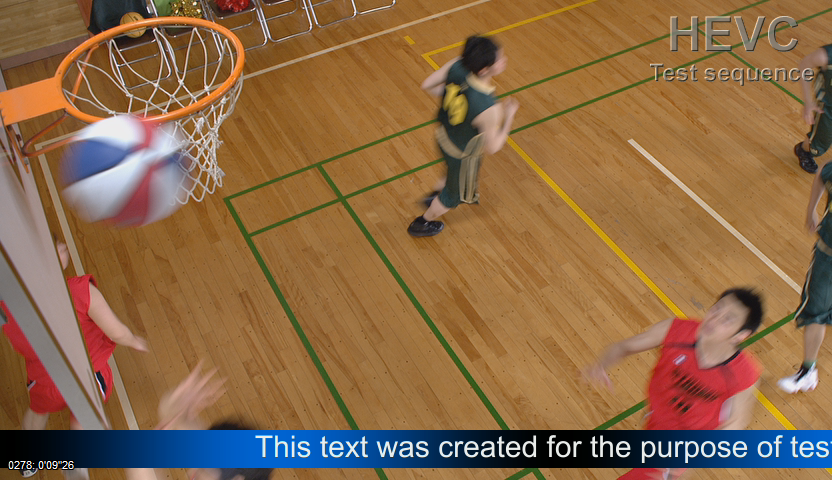
\includegraphics[height=4.0cm]{chapter6/test1.png}
    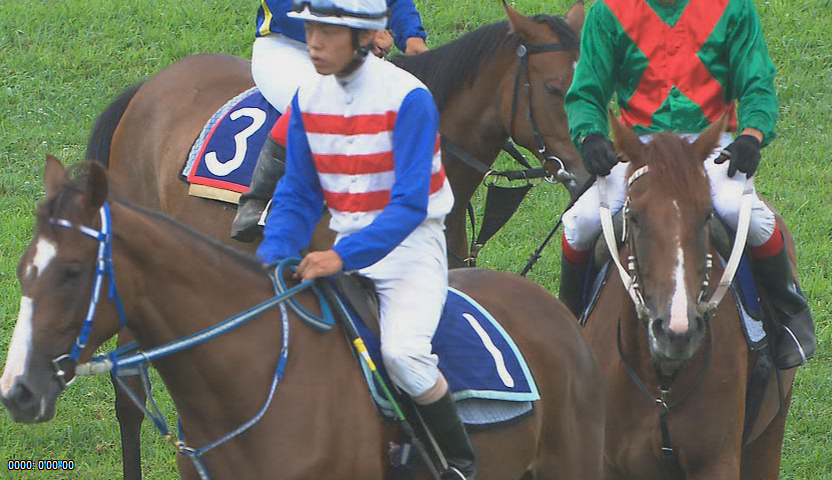
\includegraphics[height=4.0cm]{chapter6/test2.png}\\
    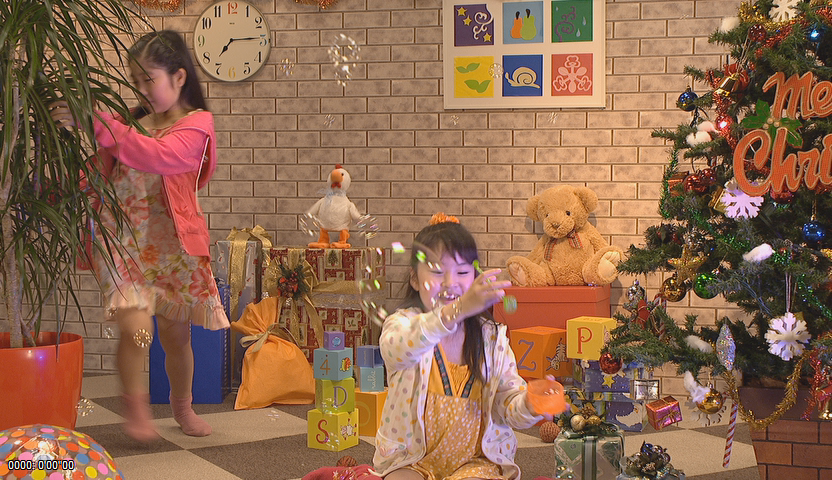
\includegraphics[height=4.0cm]{chapter6/test3.png}
    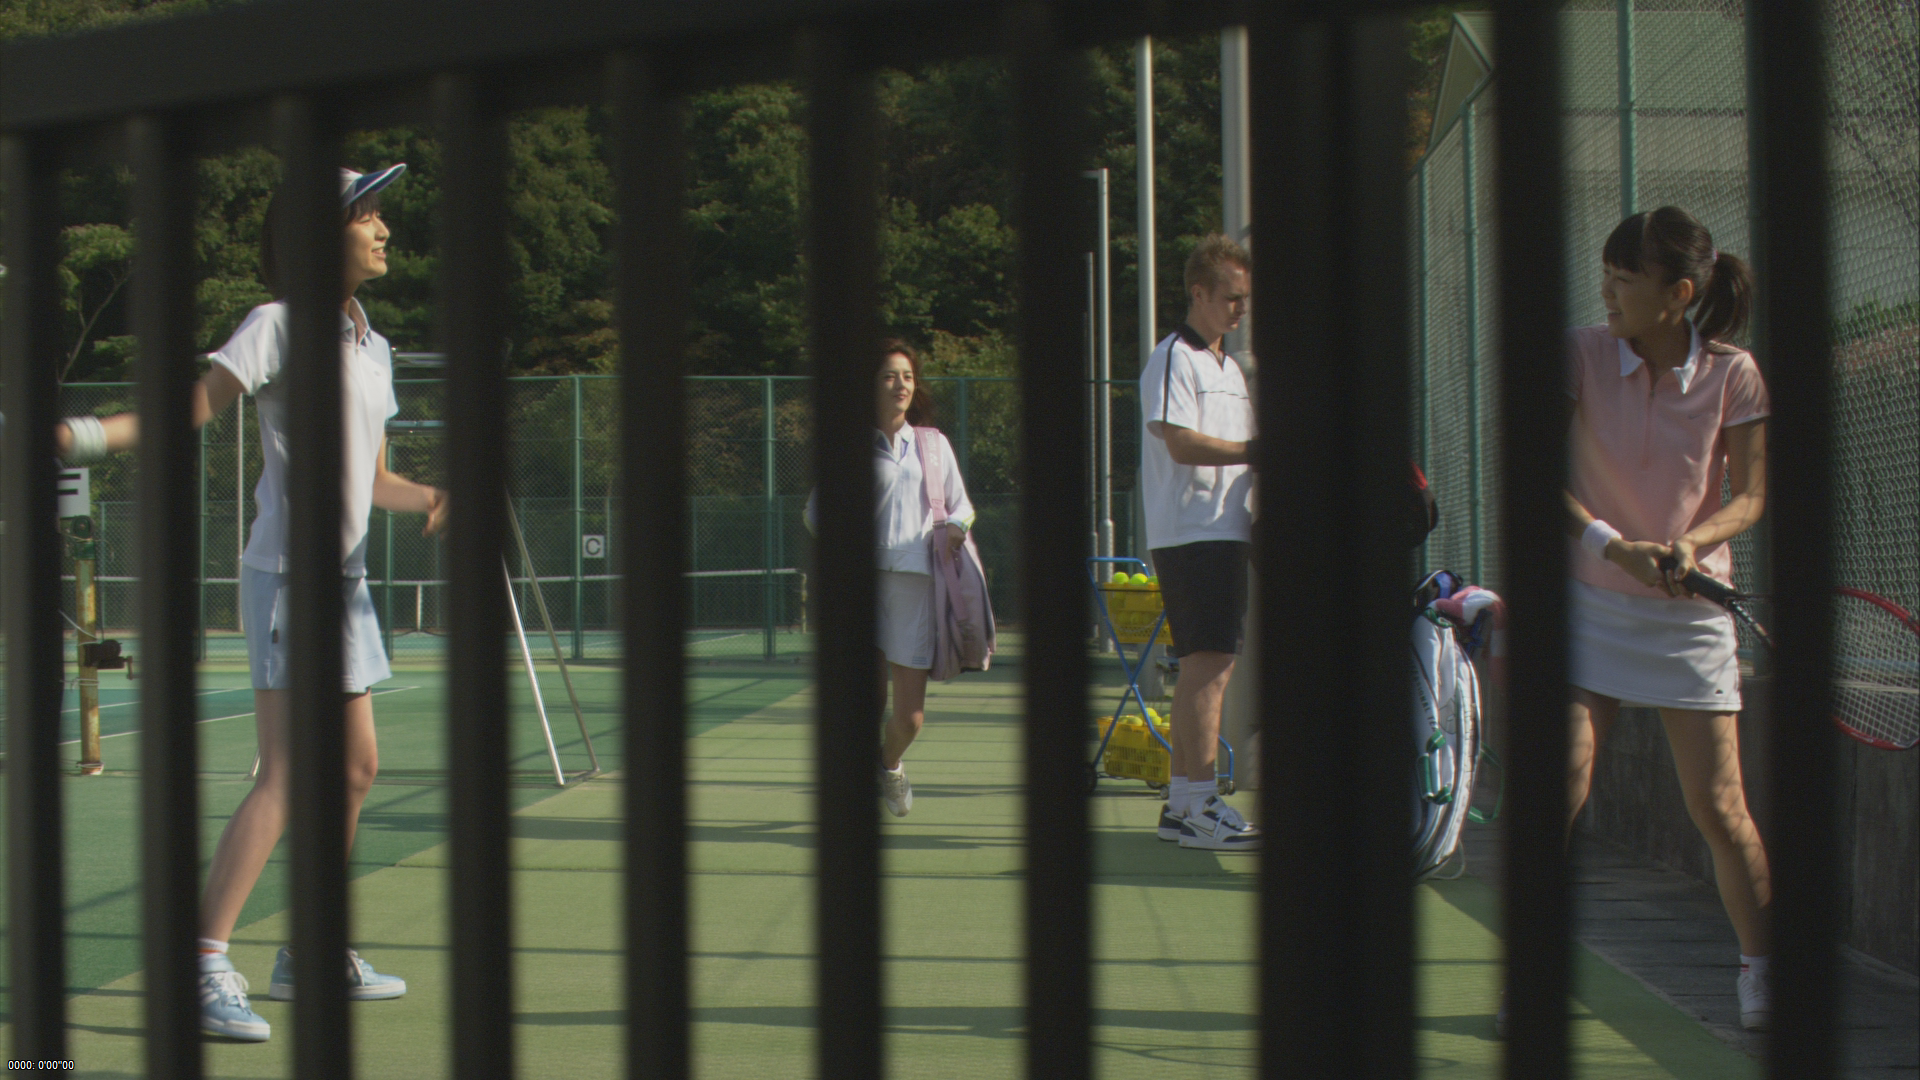
\includegraphics[height=4.0cm]{chapter6/test4.png}\\
    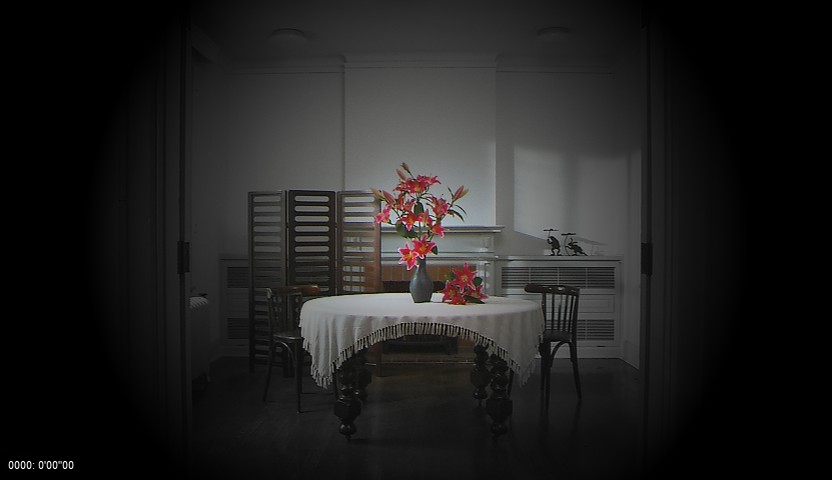
\includegraphics[height=4.0cm]{chapter6/test5.png}
\end{tabular}
\caption{Βίντεο που δοκιμάστηκαν να γίνουν encoding με τον VQ H.264.}
\label{fig:testvid}
\end{figure}

\newpage
\section{Encoding με JM H.264}
\label{section:sect62}

\indent Για να μπορούν να συγκριθούν τα αποτελέσματα των δύο encoder θα πρέπει να συμπιεστούν τα ίδια βίντεο με τον JM H.264 με τις ίδιες παραμέτρους που δεν αφορούν το VQ και προσπαθώντας να σημειωθούν τα ίδια PSNR που πέτυχε και ο VQ H.264. Αυτό πραγματοποιήθηκε δοκιμάζοντας διάφορα QP για τα καρέ I,P,B. Επειδή στον VQ H.264 παρατηρείται ότι το U,V αποδίδει πολύ καλύτερα από το Υ σε κάποια βίντεο χρειάστηκε να υπολογιστεί ο βεβαρημένος μέσος όρος $avg = 0.66*PSNRY+0.16*PSNRU+0.16*PSNRV$ έτσι ώστε να ισχύει $avg_{vq}=avg_{jm}$. Τα αποτελέσματα φαίνονται στον Πίνακα~\ref{table:jm264}.
Η ποσοστιαία διαφορά ως προς τον JM φαίνεται στον Πίνακα~\ref{table:jmvqdiff} και θα μπορούσε να χαρακτηριστεί πολύ μικρή κάτι το οποίο καθιστά την μεταξύ τους σύγκριση δίκαια.

\begin{table}[h!]
    \begin{center}
        \begin{tabular}{| l | l | l | l |}
        \hline
        Test Video & PSNR I (Y/U/V)dB  & PSNR P (Y/U/V)dB  & PSNR B (Y/U/V)dB       \\ \hline
        test1      & 36.31/38.88/38.90 & 42.01/43.95/44.54 & 43.50/44.75/45.49      \\ \hline
        test2      & 37.31/38.43/40.00 & 40.50/41.14/42.24 & 40.50/41.45/42.54      \\ \hline
        test3      & 33.94/37.24/37.85 & 38.64/40.75/41.45 & 38.45/40.51/41.25      \\ \hline
        test4      & 45.18/46.83/47.86 & 45.75/47.13/48.18 & 46.10/47.29/48.21      \\ \hline
        test5      & 39.20/46.76/47.34 & 43.94/47.66/48.28 & 45.14/49.29/49.76      \\ \hline
        \hline
        \end{tabular}
    \end{center}

    \caption{PSNR των Test videos με κωδικοποίηση στον JM H.264}
    \label{table:jm264}
\end{table}

\begin{table}[h!]
    \begin{center}
        \begin{tabular}{| l | l | l | l |}
        \hline
        Test Video & \% Diff I  & \% Diff P & \% Diff B   \\ \hline
        test1      & 1,40	    & -1,40	    & -0,93       \\ \hline
        test2      & 0,83	    & -5,11	    & -4,23       \\ \hline
        test3      & 3,53	    & -5,21	    & -5,49       \\ \hline
        test4      & 1,35	    & -0,87	    & -0,18       \\ \hline
        test5      & 1,69	    & -5,38	    & -2,76       \\ \hline
        \hline
        \end{tabular}
    \end{center}

    \caption{Διαφορές του PSNR JM-VQ. Στα θετικά πρόσημα ο JM είναι καλύτερος από τον VQ ενώ στα αρνητικά πρόσημα  το ανάποδο.}
    \label{table:jmvqdiff}
\end{table}

\newpage
\section{Αποτελέσματα των VQ H.264,JM H.264}
\label{section:sect63}

\indent Για να γίνει η σύγκριση θα υπολογιστούν τα συνολικά bits που ο JM H.264 χρειάστηκε για να αποθηκεύσει τους κβαντοποιημένους συντελεστές του μετασχηματισμού. Αυτή η πληροφορία μας παρέχεται απευθείας από την έξοδο του encoder. Αυτό γίνεται γιατί ουσιωδώς τα $VQ_{indices}$ αντιστοιχούν μόνο στην πληροφορία που  παρέχουν τα residuals, όπως και οι συντελεστές του μετασχηματισμού. Ως γνωστόν στα standard συμπίεσης βίντεο όπως το H.264 αλλά και στα mpeg1,2,4 η διαδικασία της κβαντοποίησης οδηγεί μόνο σε μηδενικούς συντελεστές, κατά συνέπεια το συγκεκριμένο block δεν κωδικοποιείται και η παρουσία σηματοδοτείται με κάποιο συγκεκριμένο flag (CBP) στο .264 αρχείο. Στην περίπτωση που όλο το macroblock αποτελείται από μηδενικά block τότε δεν κωδικοποιείται καθόλου. Στο επόμενο βήμα υπολογίστηκε ο αριθμός των Skipped macroblock και αφαιρέθηκαν 16 Υ vectors και 8 UV vectors για κάθε macroblock. Στο επόμενο βήμα πολλαπλασιάζεται η εντροπία είτε του Πίνακα~\ref{table:conentropy} (με την χρήση context) είτε του Πίνακα~\ref{fig:trainingset} (χωρίς την χρήση context) με την διάσταση του VQ για να υπολογιστεί πόσα bits χρειάζονται για κάθε block $dxd$. Τέλος πολλαπλασιάζονται τα bits που χρειάζονται ανά block με τον αριθμό των non-skipped blocks και έτσι εκτιμάται το μεγέθος που θα χρειάζονταν για την κωδικοποίηση των $VQ_{indices}$ μετά απο συμπίεσης. Αναμένεται μετά από χρήση είτε πινάκων Huffman είτε με την χρήση CABAC, να σημειωθούν τα αποτελέσματα τα οποία φαίνονται στο Σχήμα~\ref{fig:compare1}.

\begin{figure}[H]
    \centering
    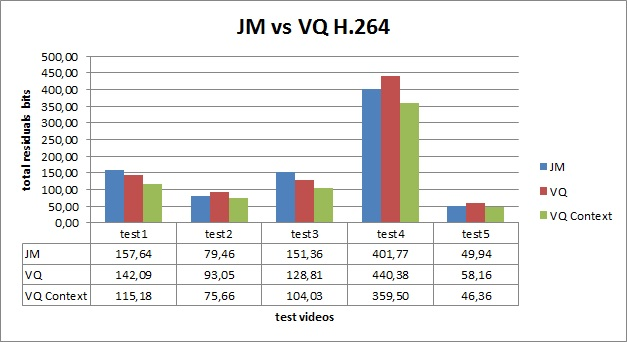
\includegraphics[width=0.8\textwidth]{chapter6/compare1.jpg}
    \caption{Σύγκριση των bits του JM H.264 και VQ H.264 με context entropy και χωρίς context.}
    \label{fig:compare1}
\end{figure}

\indent Εκτός από την σύγκριση της αποδοτικότητας της συμπίεσης έγινε προσπάθεια να συγκριθούν και οι χρόνοι κωδικοποίησης και αποκωδικοποίησης. Όπως αναφέρθηκε ο VQ Η.264 κάνει όλη την άχρηστη για αυτόν δουλειά του μετασχηματισμού, κβαντοποίησης, αντίστροφου μετασχηματισμού, αντίστροφης κβαντοποίησης. Συνεπώς, χρησιμοποιήθηκε το Intel VTune για να βρεθεί ο χρόνος αυτόν των συναρτήσεων και να αφαιρεθούν από τον συνολικό. Έτσι έγινε μια καλή προσέγγιση των επιδόσεων του VQ H.264 και η σύγκρισή με τον JM H.264 φαίνεται στο Σχήμα~\ref{fig:compare2} και στο Σχήμα~\ref{fig:compare3}. Παρατηρείται ότι στον VQ H.264 encoder υπάρχει αύξηση της πολυπλοκότητας το οποίο οφείλεται αποκλειστικά στην αναζήτηση FastNN. Στον VQ H.264 decoder παρατηρείται μια αναίσθητη διαφορά.

 \begin{figure}[H]
    \centering
    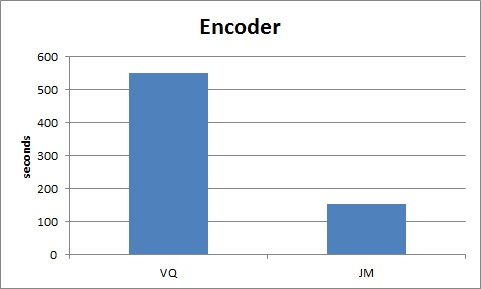
\includegraphics[width=0.8\textwidth]{chapter6/compare2.jpg}
    \caption{Σύγκριση του χρόνου εκτέλεσης των encoder JM H.264 και VQ H.264.}
    \label{fig:compare2}
\end{figure}

 \begin{figure}[H]
    \centering
    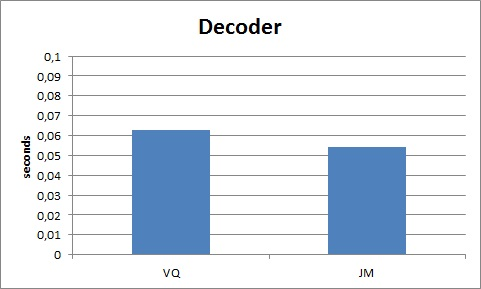
\includegraphics[width=0.8\textwidth]{chapter6/compare3.jpg}
    \caption{Σύγκριση του χρόνου εκτέλεσης των decoder JM H.264 και VQ H.264.}
    \label{fig:compare3}
\end{figure} 

%\chapter{Συμπεράσματα}
\label{chapter:chap7}

\section{VQ H.264 vs JM H.264}
\label{section:sect63}

\indent Από το Σχήμα~\ref{fig:compare1} βλέπουμε πως ο VQ H.264 χρησιμοποιεί κατά μέσο όρο 17\% λιγότερα bits από τον JM H.264 στα βίντεο που δοκιμάστηκε. Επίσης φαίνεται να υπάρχει ακόμα μεγαλύτερο κέρδος στα βίντεο που περιέχουν γρήγορη κίνηση, πράγμα που τα κάνει δύσκολο να κωδικοποιηθούν, τέτοια βίντεο είναι τα test1,test3 με κέρδος 27\% και 31\% αντίστοιχα. Σε αντίθεση στα βίντεο test2,test4,test5 που δεν δυσκολεύουν ιδιαίτερα τον encoder παρατηρείται ότι είναι μικρότερο.

\indent Θα πρέπει να ληφθεί υπόψιν  ότι το VQ έχει πολλά περιθώρια βελτίωσης αν μεγαλώσει το training set. Με το τρέχον training set παρατηρήθηκε πως σε κάποια βίντεο και ειδικά στα I frames δεν έχει καλή απόδοση ο VQ. Αυτό μπορεί να βελτιωθεί απλά και μόνο συμπεριλαμβάνοντας αυτά ή παραπλήσια βίντεο στο training set. Το θετικό σε αυτή την διαδικασία είναι ότι δεν χρειάζεται να γίνει τρέξιμο του training από την αρχή, αρκεί να δωθούν σαν αρχικά clusters αυτά που ήδη υπάρχουν και έτσι να  μην γίνει η αρχικοποίηση αλλά και πολλά iterations του αλγορίθμου. Επομένως, ένας encoder που δουλεύει με VQ θα μπορεί να ανανεώνει τα codebooks του ανά κάποιο χρονικό διάστημα και θα επιλέγει αυτά που το βίντεο κωδικοποιήθηκε μέσω κάποιου version header μέσα στο βίντεο.

\indent Ένα πρόβλημα που εμφανίζεται είναι η μεγάλη ανομοιομορφία του PSNR μεταξύ I,P,B αλλά και Y,UV. Δηλαδή στο βίντεο test1  το I είναι στα 35dB ενώ τα P,B στα 43dB,45dB αντίστοιχα. Αυτή η διαφορά είναι αρκετά μεγάλη και για να μειωθεί θα μπορούσαν να χρησιμοποιηθούν codebooks με διαφορετικό μέγεθος για κάθε συνιστώσα I,P,B|Y,UV. Έτσι λοιπόν αν χρησιμοποιηθούν Inter codebook μήκους 32768 για το test1 θα χρειάζονταν λιγότερα bits για να αποθηκευτούν  τα $VQ_{indices}$ αλλά ταυτόχρονα θα μειωνόταν και το PSNR. Επομένως, στο VQ το μέγεθος του codebook $k$ λειτουργεί σαν ρυθμιστής ποιότητας παίζοντας τον ρόλο που παίζει το QP στο scalar quantization. Δεν πραγματοποιήθηκαν μετρήσεις πάνω σε αυτόν το τομέα, αλλά αφήνονται σαν μια πολύ σημαντική προσθήκη για την ολοκλήρωση του VQ H.264.

\indent Όπως φαίνεται στο Σχήμα~\ref{fig:compare2}  ο VQ Encoder είναι 3.5 φορές πιο αργός από τον JM, κάτι που οφείλεται στο κόστος του αλγορίθμου FastNN. Αντιθέτως, ο VQ Decoder στο Σχήμα~\ref{fig:compare3} είναι στα ίδια επίπεδα με τον JM Decoder. Αυτό που είναι σημαντικό είναι να η ύπαρξη γρήγορων decoders καθώς μπαίνουν σε φορητές συσκευές που ενδιαφέρει η ενεργειακή απόδοση. Έτσι ένας VQ Decoder μπορεί να βελτιστοποιηθεί χρησιμοποιώντας μικρές και γρήγορες μνήμες όπου θα αποθηκεύονται τα codebooks. Ένα ενεργοβόρο και ακριβό βοηθητικό κύκλωμα που επιταχύνει την διαδικασία του αντίστροφου μετασχηματισμού και της αντίστροφης κβαντοποίησης μετατρέπεται σε μια γρήγορη, χαμηλής κατανάλωσης, φθηνή μνήμη. Η μνήμη που χρειάζεται για να αποθηκευτούν τα VQ codebooks είναι αρκετά μικρή. Στην διπλωματική αυτή για ένα codebook χρείαζεται συνολικά $k*d*2 = 4MB$ με $k=65536$ και $d=16$ επομένως για τα $4$ codebooks χρειαζόμαστε $16MB$ τα $2 bytes$ προκύπτουν επείδη $k=65536=2^{16}$ άρα τα indices χρείαζονται $16  bits = 2  bytes$ για να αποθηκευτούν.

\section{Πιθανές προσθήκες}
\label{section:sect63}

\indent Επειδή το VQ έδειξε στην παρούσα διπλωματική εργασία ότι αξίζει παραπάνω προσοχή, παρατίθενται παρακάτω κάποιες προτάσεις που θα αυξήσουν την απόδοτικότητα του.

\begin{itemize}

    \item Χρήση διαφορετικού μεγέθους codebooks για τις διάφορες συνιστώσες Y,UV, καθώς και παραγωγή codebooks για διάφορες ποιότητες ($k$).

    \item Προσαρμογή του πυρήνα του JM H.264 έτσι ώστε στον encoder να μην γίνεται μετασχηματισμός και κβαντοποίηση αλλά απευθείας VQ και έπειτα να κωδικοποιούνται τα $VQ_{indices}$ με την χρήση των contexts και την σωστή χρήση κωδικοποιητή εντροπίας. Με αυτόν τον τρόπο, ο decoder θα δέχεται μόνο ένα αρχείο με τα $VQ_{indices}$ κωδικοποιημένα εντός του αρχείου H.264 και θα παράγει το αποκωδικοποιημένο βίντεο.

    \item Παραγωγή του training set από βίντεο που έχουν παραχθεί από VQ H.264, κατά αυτόν τον τρόπο αναμένεται παραγωγή καλύτερης ποιότητας codebook τα οποία μπορούν με την σειρά τους να παράγουν ακόμα καλύτερης ποιότητας training set τα οποία θα συγκλίνουν μετά από έναν συγκεκριμένο αριθμό επαναλήψεων.
    
    Δοκιμή παραγωγής του training set από βίντεο που έχουν ήδη κωδικοποιηθεί με την χρήση VQ. Χρήση αυτών των νέων codebooks για να γίνει VQ και πάλι στο βίντεο για να δειχθεί αν έτσι βελτιώνεται η ποιότητα του VQ. Μπορεί αυτό το loop να χρειαστεί να γίνει παραπάνω από μία φόρες
\end{itemize}

%\backmatter

%\cleardoublepage
%\bibliographystyle{plain}
%\bibliography{Bibliography/ThesisBibliography}
\nocite{*}

\end{document} 